\documentclass[a4paper, 12pt]{article}

\usepackage[table,xcdraw]{xcolor}
\usepackage{enumerate}
\usepackage{graphicx}
\usepackage[T5]{fontenc}
\usepackage[utf8]{inputenc}
\usepackage[margin = 2cm]{geometry}
\usepackage{amsfonts, amsmath, amssymb}
\usepackage[none]{hyphenat}
\usepackage{fancyhdr}
\usepackage{float}
\usepackage{hyperref}
\usepackage{caption}
\usepackage[nottoc, notlot, notlof]{tocbibind}

% for code section
\usepackage{listings}

% for sub-figure
\usepackage{subcaption}
% \usepackage{rotating}
% \usepackage{tikz}

\captionsetup[table]{skip=5pt}
\pagestyle{fancy}
\fancyhead[L]{Trường Đại học Khoa học Tự nhiên - ĐHQG TP.HCM}
\fancyhead[R]{Nhóm 17}

\begin{document}

\begin{titlepage}
    \begin{center}
        \vspace*{1cm}
        \Large\textbf{Đại học Quốc gia TP. HCM\\Trường Đại học Khoa học Tự nhiên}\\

        \vfill
        \line(1,0){450}\\[4mm]
        \LARGE\textbf{\MakeUppercase{Báo cáo Lab 02\\ Trực quan hóa dữ liệu với Tableau}}\\[3mm]
        \Large{Trực quan hoá dữ liệu (CSC10108)}\\[3mm]
        \Large{Nhóm 17}
        \line(1,0){430}\\
        \vfill

        \vfill
        TP Hồ Chí Minh, ngày 23/05/2021
    \end{center}
\end{titlepage}

\tableofcontents
\thispagestyle{empty}
\clearpage

\section{Thông tin nhóm}
    \begin{table}[H]
        \begin{tabular}{|c|c|l|c|c|}
        \hline
        STT & MSSV     & \multicolumn{1}{c|}{Họ tên} & Email                         & SĐT        \\ \hline
        1   & 18120078 & Ngô Phù Hữu Đại Sơn         & 18120078@student.hcmus.edu.vn & 0919070940 \\ \hline
        2   & 18120201 & Nguyễn Bảo Long             & 18120201@student.hcmus.edu.vn & 0981850699 \\ \hline
        3   & 18120227 & Phạm Văn Minh Phương             & 18120227@student.hcmus.edu.vn & 0981850699 \\ \hline
        4   & 18120253 & Mai Ngọc Tú             & 18120253@student.hcmus.edu.vn & 0981850699 \\ \hline
        5   & 1712424 & Hàn Văn Gia Hiên            & 1712424@student.hcmus.edu.vn & 0911572108 \\ \hline
        \end{tabular}
        \caption{Bảng danh sách thành viên nhóm}
    \end{table}
    \clearpage

    \section{Phân tích hoàn thiện yêu cầu}

    \subsection{Tổng quan mức độ hoàn thành mỗi yêu cầu}

    \begin{table}[H]
        \begin{tabular}{|c|l|l|c|}
        \hline
        STT & \multicolumn{1}{c|}{Yêu cầu} & \multicolumn{1}{c|}{Công việc}                                                & Hoàn thành (\%) \\ \hline
        1 & Tìm hiểu công cụ Tableau      & \begin{tabular}[c]{@{}l@{}}- Giới thiệu Tableau\\ - Giới thiệu tính năng kèm ví dụ\end{tabular}              & 100/100\\ \hline
        2 & Trực quan sử dụng Tableau & \begin{tabular}[c]{@{}l@{}}- Trực quan các biến, các mối quan hệ, \\giải thích ý nghĩa, nhận xét biểu đồ\end{tabular}                          & 90/100 \\ \hline\end{tabular}
        \caption{Bảng phân tích đóng góp cá nhân}
    \end{table}

    \subsection{Mức độ hoàn thành của thành viên nhóm}

    \begin{table}[H]
        \begin{tabular}{|c|l|l|c|}
        \hline
        STT & \multicolumn{1}{c|}{Họ tên} & \multicolumn{1}{c|}{Công việc tham gia}                                                & Hoàn thành (\%) \\ \hline
        1 & Ngô Phù Hữu Đại Sơn      & \begin{tabular}[c]{@{}l@{}}- Biểu diễn Word Cloud, Line Chart, Tree \\Map, World Map, Bar Chart, Dashboard\\ - Nhận xét dữ liệu World Map, Corelation\\ Matrix\end{tabular}              & 100/100 \\ \hline
        2 & Nguyễn Bảo Long & \begin{tabular}[c]{@{}l@{}}- Biểu diễn Stacked Bar Chart, Corelation\\ Matrix \\ - Tổng hợp báo cáo\end{tabular}                          & 100/100 \\ \hline
        5 & Phạm Văn Minh Phương        & \begin{tabular}[c]{@{}l@{}}- Biểu diễn Scatter Plot đa biến\\ - Nhận xét dữ liệu Scatter Plot đa biến\end{tabular} & 100/100 \\ \hline
        5 & Mai Ngọc Tú       & \begin{tabular}[c]{@{}l@{}}- Tìm hiểu Tableau\\ - Nhận xét dữ liệu biểu đồ World Map,\\ Bar Plot, Tree Map \end{tabular} & 100/100 \\ \hline
        5 & Hàn Văn Gia Hiên       & \begin{tabular}[c]{@{}l@{}}- Tìm hiểu Tableau\\ - Nhận xét dữ liệu biểu đồ Line Chart,\\ Stacked Bar Chart \end{tabular} & 100/100 \\ \hline
        \end{tabular}
        \caption{Bảng phân tích tỷ lệ hoàn thành công việc}
    \end{table}
    \clearpage

\section{Tìm hiểu công cụ Tableau}

\subsection{Giới thiệu}

\begin{itemize}
    \item Tableau là phần mềm hỗ trợ phân tích và trực quan hóa dữ liệu, được dùng nhiều trong lĩnh vực Business Intelligence nhằm xây dựng nền tảng số và phân tích dữ liệu cho doanh nghiệp
    \item Các chức năng chính của Tableau bao gồm:
    \begin{itemize}
        \item Kết nối với nhiều nguồn dữ liệu (định dạng excel, định dạng *.csv, các hệ quản trị cơ sở dữ liệu,...) và làm việc đồng thời trên trên các nguồn dữ liệu này
        \item Cung cấp công cụ để làm sạch và chuẩn bị dữ liệu cho việc phân tích
        \item Dễ dàng tạo các phân tích dữ liệu bằng các thao tác đơn giản
        \item Cung cấp các phương pháp phân tích phổ biến khi xử lý số liệu như hồi quy tuyến tính để dự đoán xu hướng, biểu diễn đường trung bình, đường trung vị, cluster dữ liệu,... với thao tác thực hiện rất trực quan
        \item Tạo các tương tác lọc, rút trích, drill-up, drill-down hoặc các tham số xử lý dữ liệu ngay trên các biểu đồ
        \item Phân tích dữ liệu dựa trên vị trí địa lý (trực quan các khu vực tỉnh, thành phố, quốc gia) với hỗ trợ hầu hết các quốc gia trên thế giới
        \item Hỗ trợ người dùng tạo ra các dashboard quản trị và các story của dữ liệu để thực hiện tốt quá trình phân tích kinh doanh
        \item Vận hành tốt trên các thiết bị di động iOS \& Android. Do đó người dùng có thể cập nhật phân tích dữ liệu mọi lúc mọi nơi
        \item Chia sẻ các phân tích dữ liệu với đồng nghiệp
        \item Linh động chọn môi trường triển khai với on-premise, on-cloud với full cloud trên nền tảng của Tableau, các public cloud của Amazon, Google, Microsoft. Hỗ trợ các hệ điều hành Windows, Linux, macOS,...
    \end{itemize}

    \item Lợi ích của Tableau:
    \begin{itemize}
        \item Giúp người dùng nhanh chóng tổng hợp, phân tích và đưa ra các phân tích dưới góc nhìn của doanh nghiệp về hoạt động kinh doanh
        \item Xây dựng môi trường làm việc cộng tác, số hóa trên một cơ sở dữ liệu cho doanh nghiệp
        \item Việc xây dựng Data Warehouse là không nhất thiết
        \item Triển khai nhanh, khả năng tiếp cận của người dùng nhanh, giảm thiểu tối đa chi phí triển khai, dễ dàng mở rộng theo mô hình và độ lớn nghiệp vụ của doanh nghiệp
    \end{itemize}

    \item Cài đặt
    \begin{itemize}
        \item Truy cập \url{https://www.tableau.com/} để tải về bản cài đặt
        \item Ứng dụng cho phép dùng thử 14 ngày hoặc đăng ký Tableau for Students đối với mục đích giảng dạy và học tập
        \item Khởi chạy bản cài đặt và làm theo các hướng dẫn của phần mềm
    \end{itemize}
\end{itemize}

\subsection{Các tính năng chính của Tableau}

\begin{itemize}
    \item Báo cáo này trình bày các tính năng cơ bản nhất của phầm mềm Tableau. Để biết thêm chi tiết, vui lòng truy cập đường dẫn \url{https://www.tableau.com/support/help}
    \item Người viết giả định rằng người đọc đã có một số kiến thức cơ bản về biểu diễn dữ liệu (các dạng biểu đồ, các trường hợp dùng các dạng biểu đồ,...)
    \item Các tính năng này được thực hiện trên bộ dữ liệu mẫu "Sample - Superstore" do Tableau cung cấp
\end{itemize}

\subsubsection{Chọn bảng dữ liệu và tạo Work Sheet}

\begin{itemize}
    \item Tableau đã thực hiện kết bảng sẵn đối với bộ dữ liệu mẫu. Tuy nhiên, ta hoàn toàn có thể thực hiện kết bảng thủ công như hình minh họa
    \begin{figure}[H]
        \begin{center}
            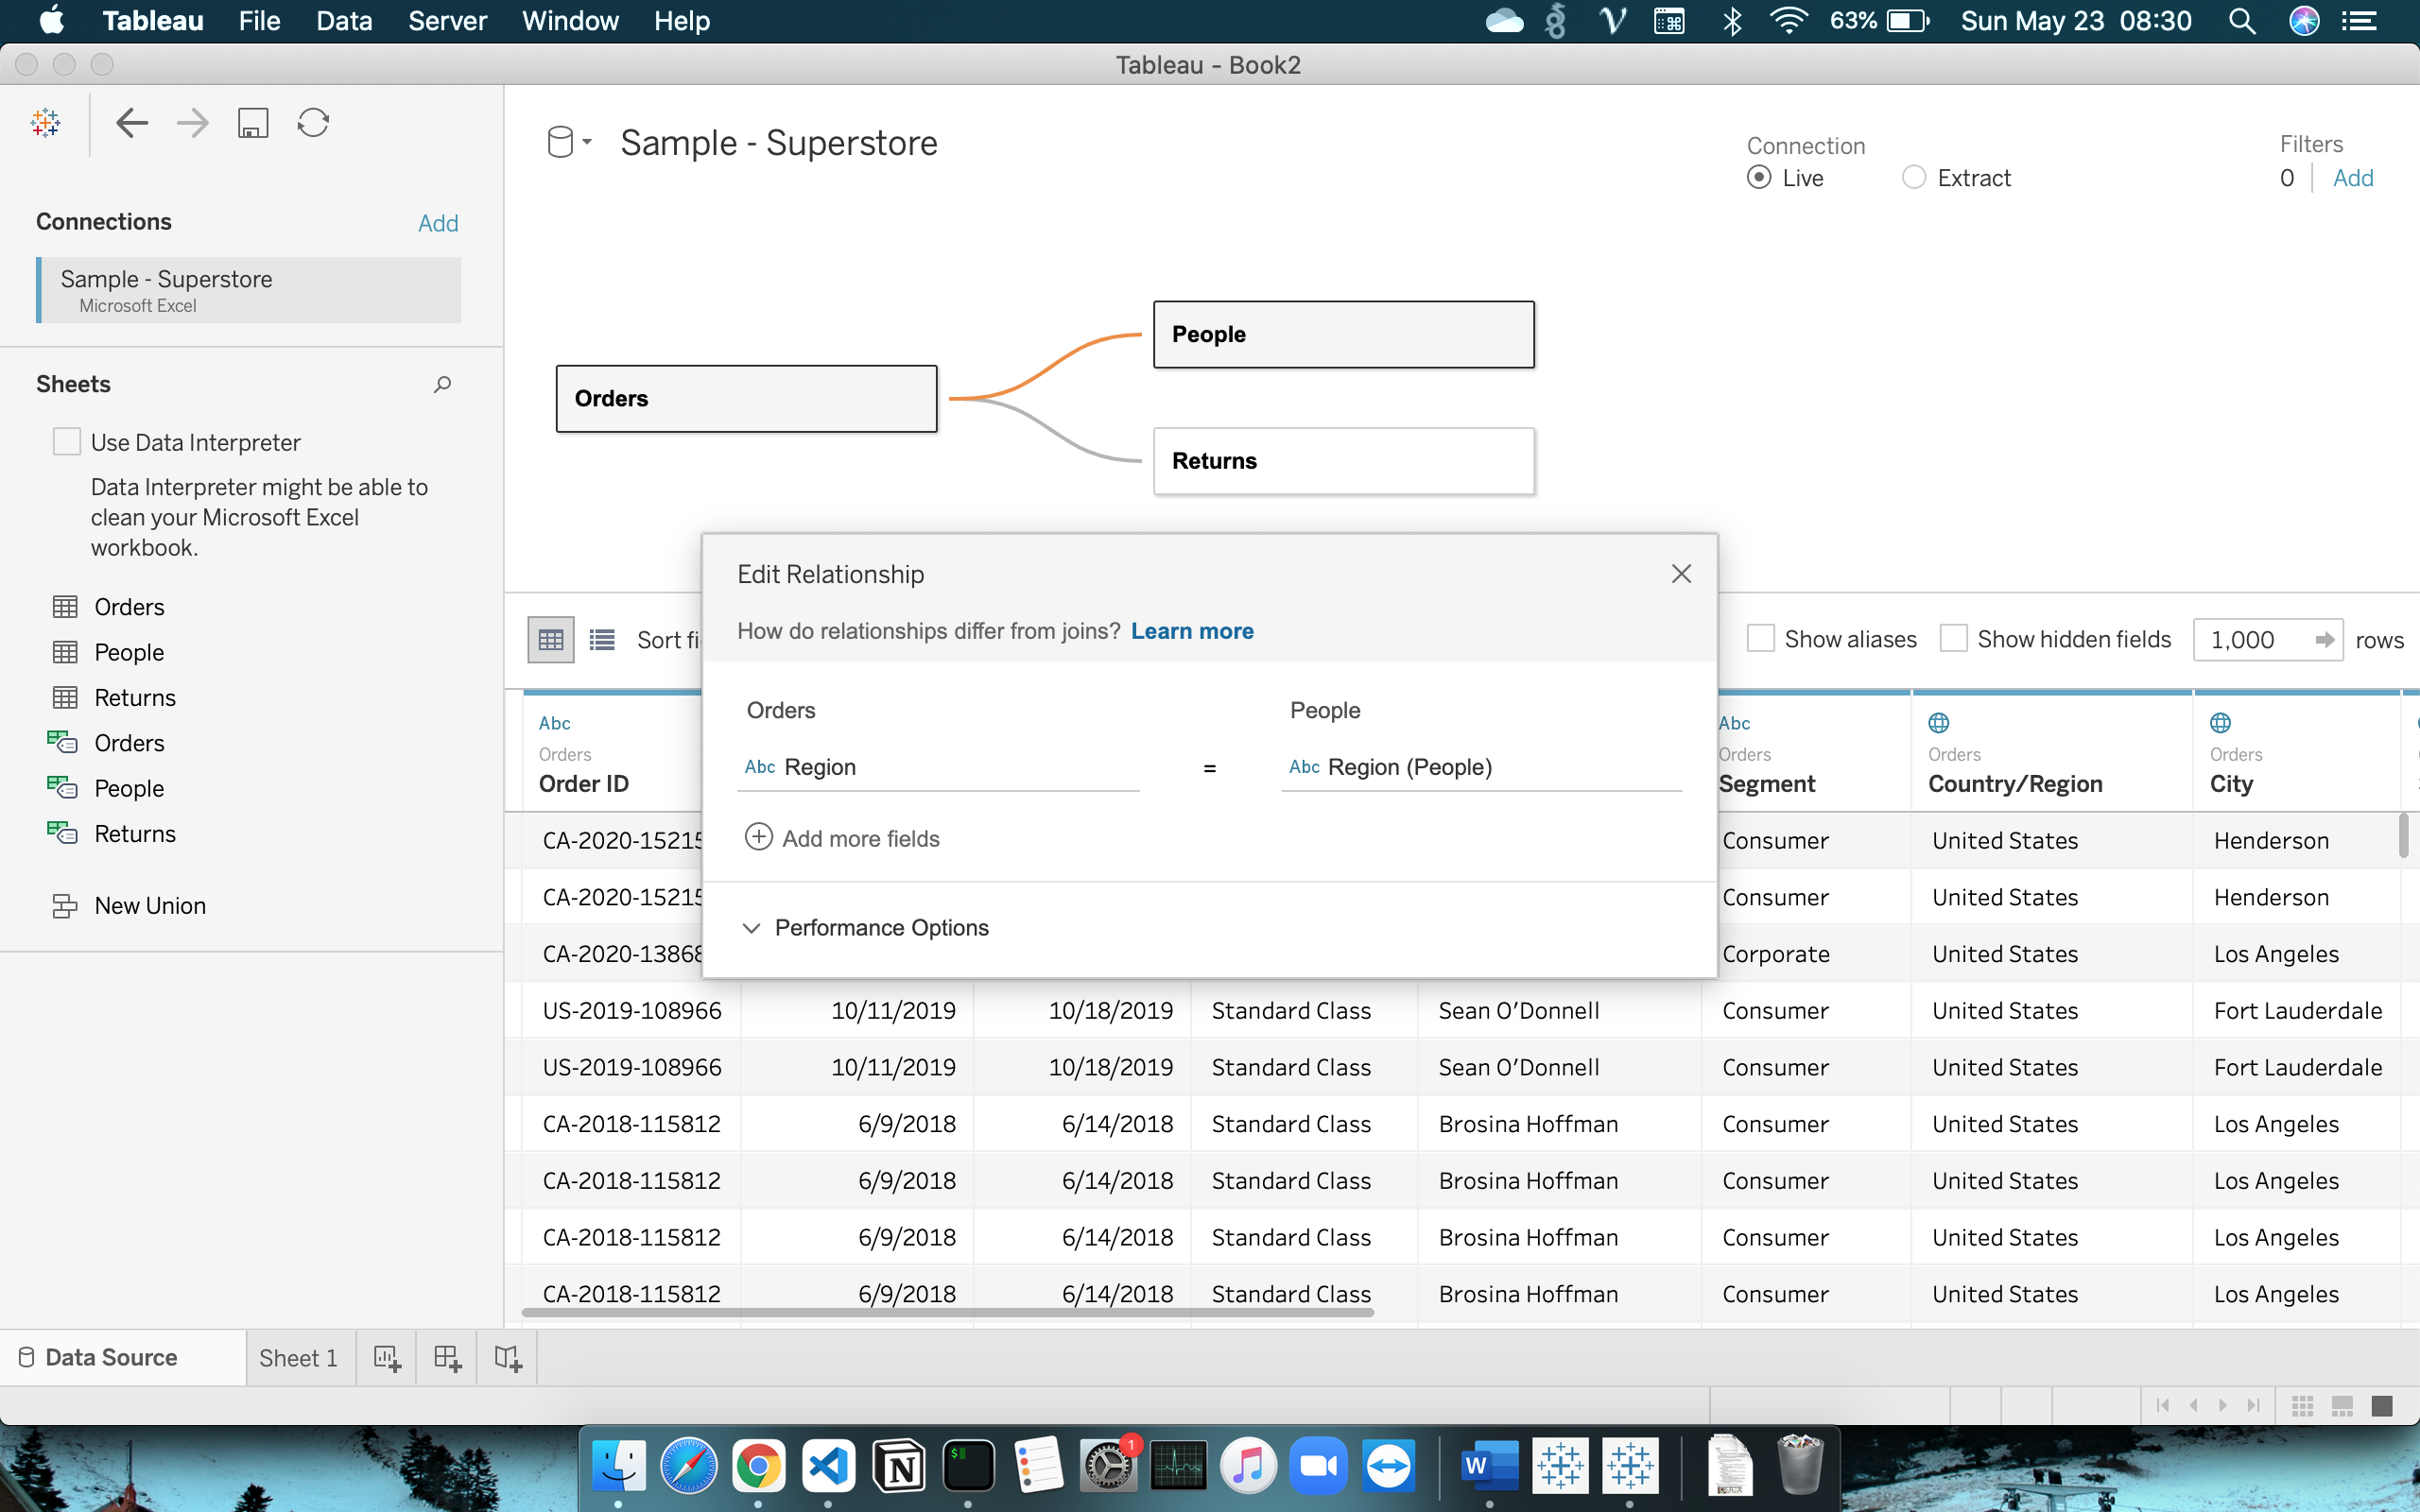
\includegraphics[scale=0.3]{img/joinTable.png}
            \caption{Cấu hình bộ dữ liệu để làm việc}
        \end{center}
    \end{figure}

    \item Để thực hiện trực quan và phân tích, ta cần tạo một \textbf{Work Sheet}. Các thành phần chính của 1 work sheet bao gồm
    \begin{figure}[H]
        \begin{center}
            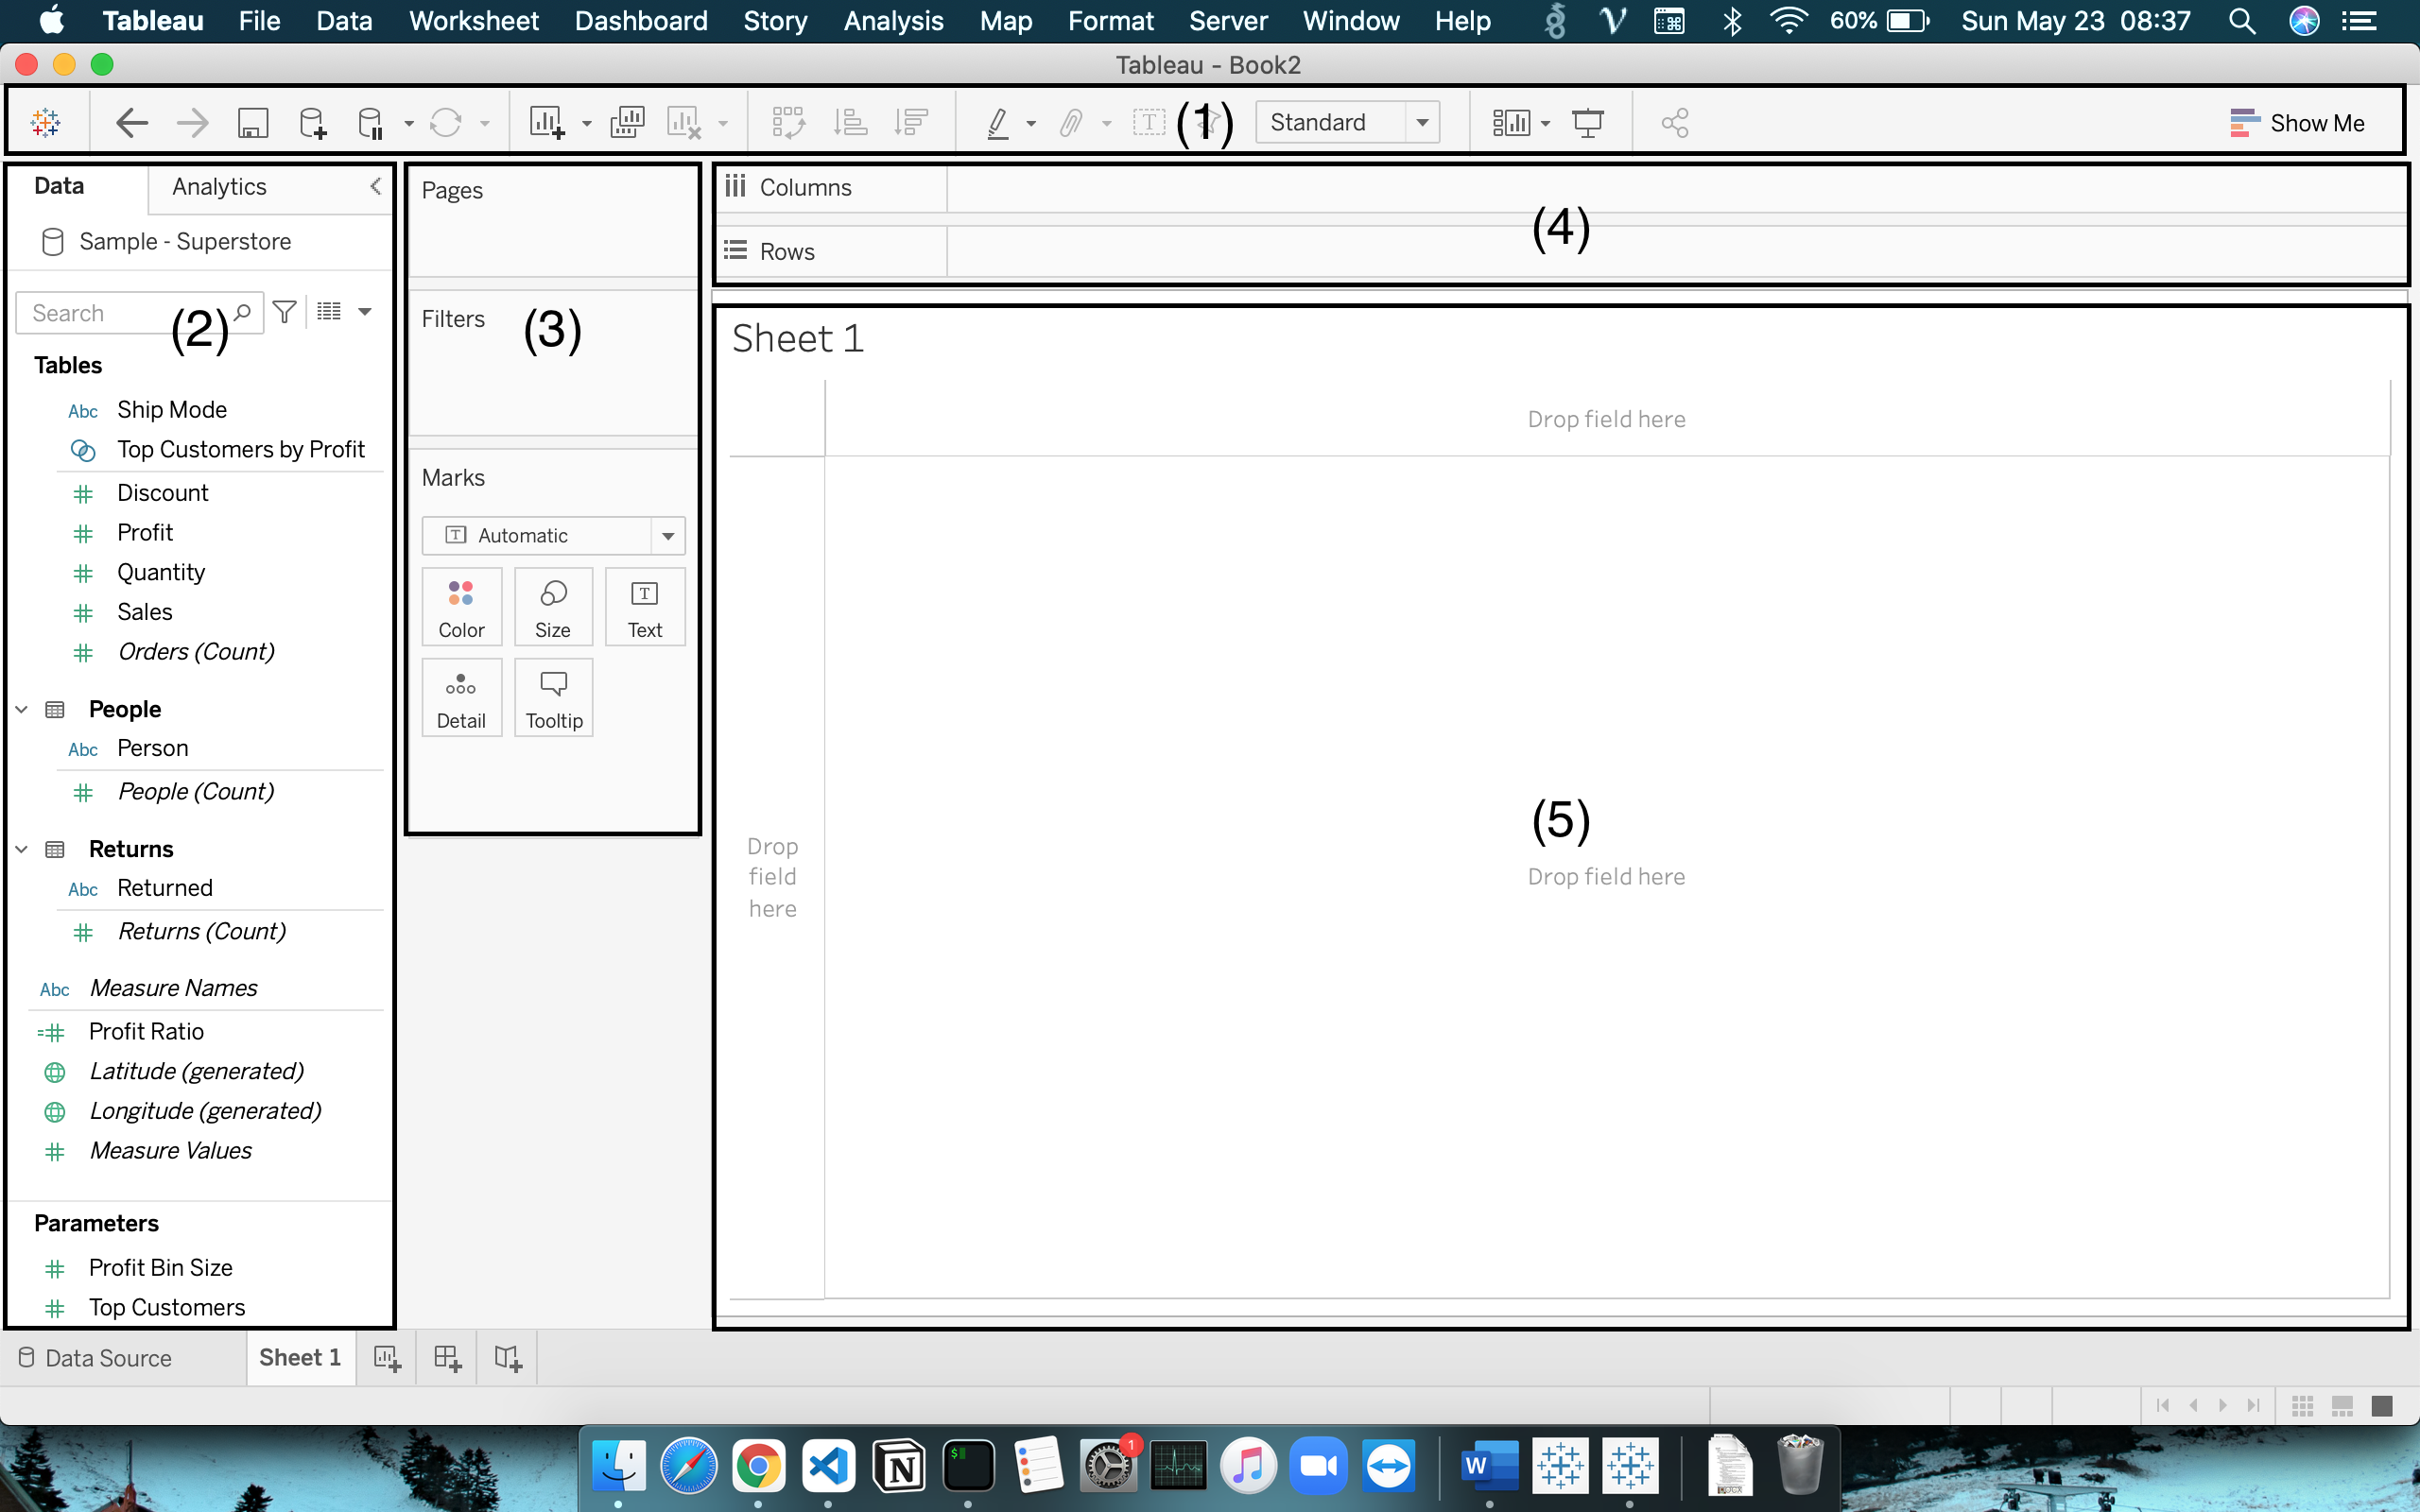
\includegraphics[scale=0.3]{img/newSheet.png}
            \caption{Thành phần của một work sheet}
        \end{center}
    \end{figure}

    \begin{itemize}
        \item (1): Các công cụ thường sử dụng trong việc cấu hình biểu đồ
        \item (2): Khung Dữ liệu \& Phân tích. Được chia thành 2 tabs
        \begin{itemize}
            \item Tab Data chứa các trường dữ liệu trong bộ dữ liệu
            \item Tab Analytics chứa các phân tích dữ liệu cơ bản bao gồm: Phân tích tóm tắt (biểu diễn các đường hằng số, trung bình, trung vị,...); Phân tích bằng thuật toán (biểu diễn xu hướng, dự đoán, gom cụm,...); Phân tích khác (do người dùng tự định nghĩa)
        \end{itemize}

        \item (3): Bộ lọc và điều chỉnh dữ liệu
        \item (4): Khung chứa dữ liệu được trực quan, bao gồm 2 khung: Rows và Columns
        \item (5): Khung chứa biểu đồ
    \end{itemize}
\end{itemize}

\subsubsection{Vẽ demo biểu đồ đường, biểu đồ cột và bản đồ}

\begin{itemize}
    \item Biểu đồ cột: Loại biểu đồ thể hiện giá trị thực của dữ liệu. Phục vụ so sánh, phân tích xu hướng,...
    \begin{figure}[H]
        \begin{center}
            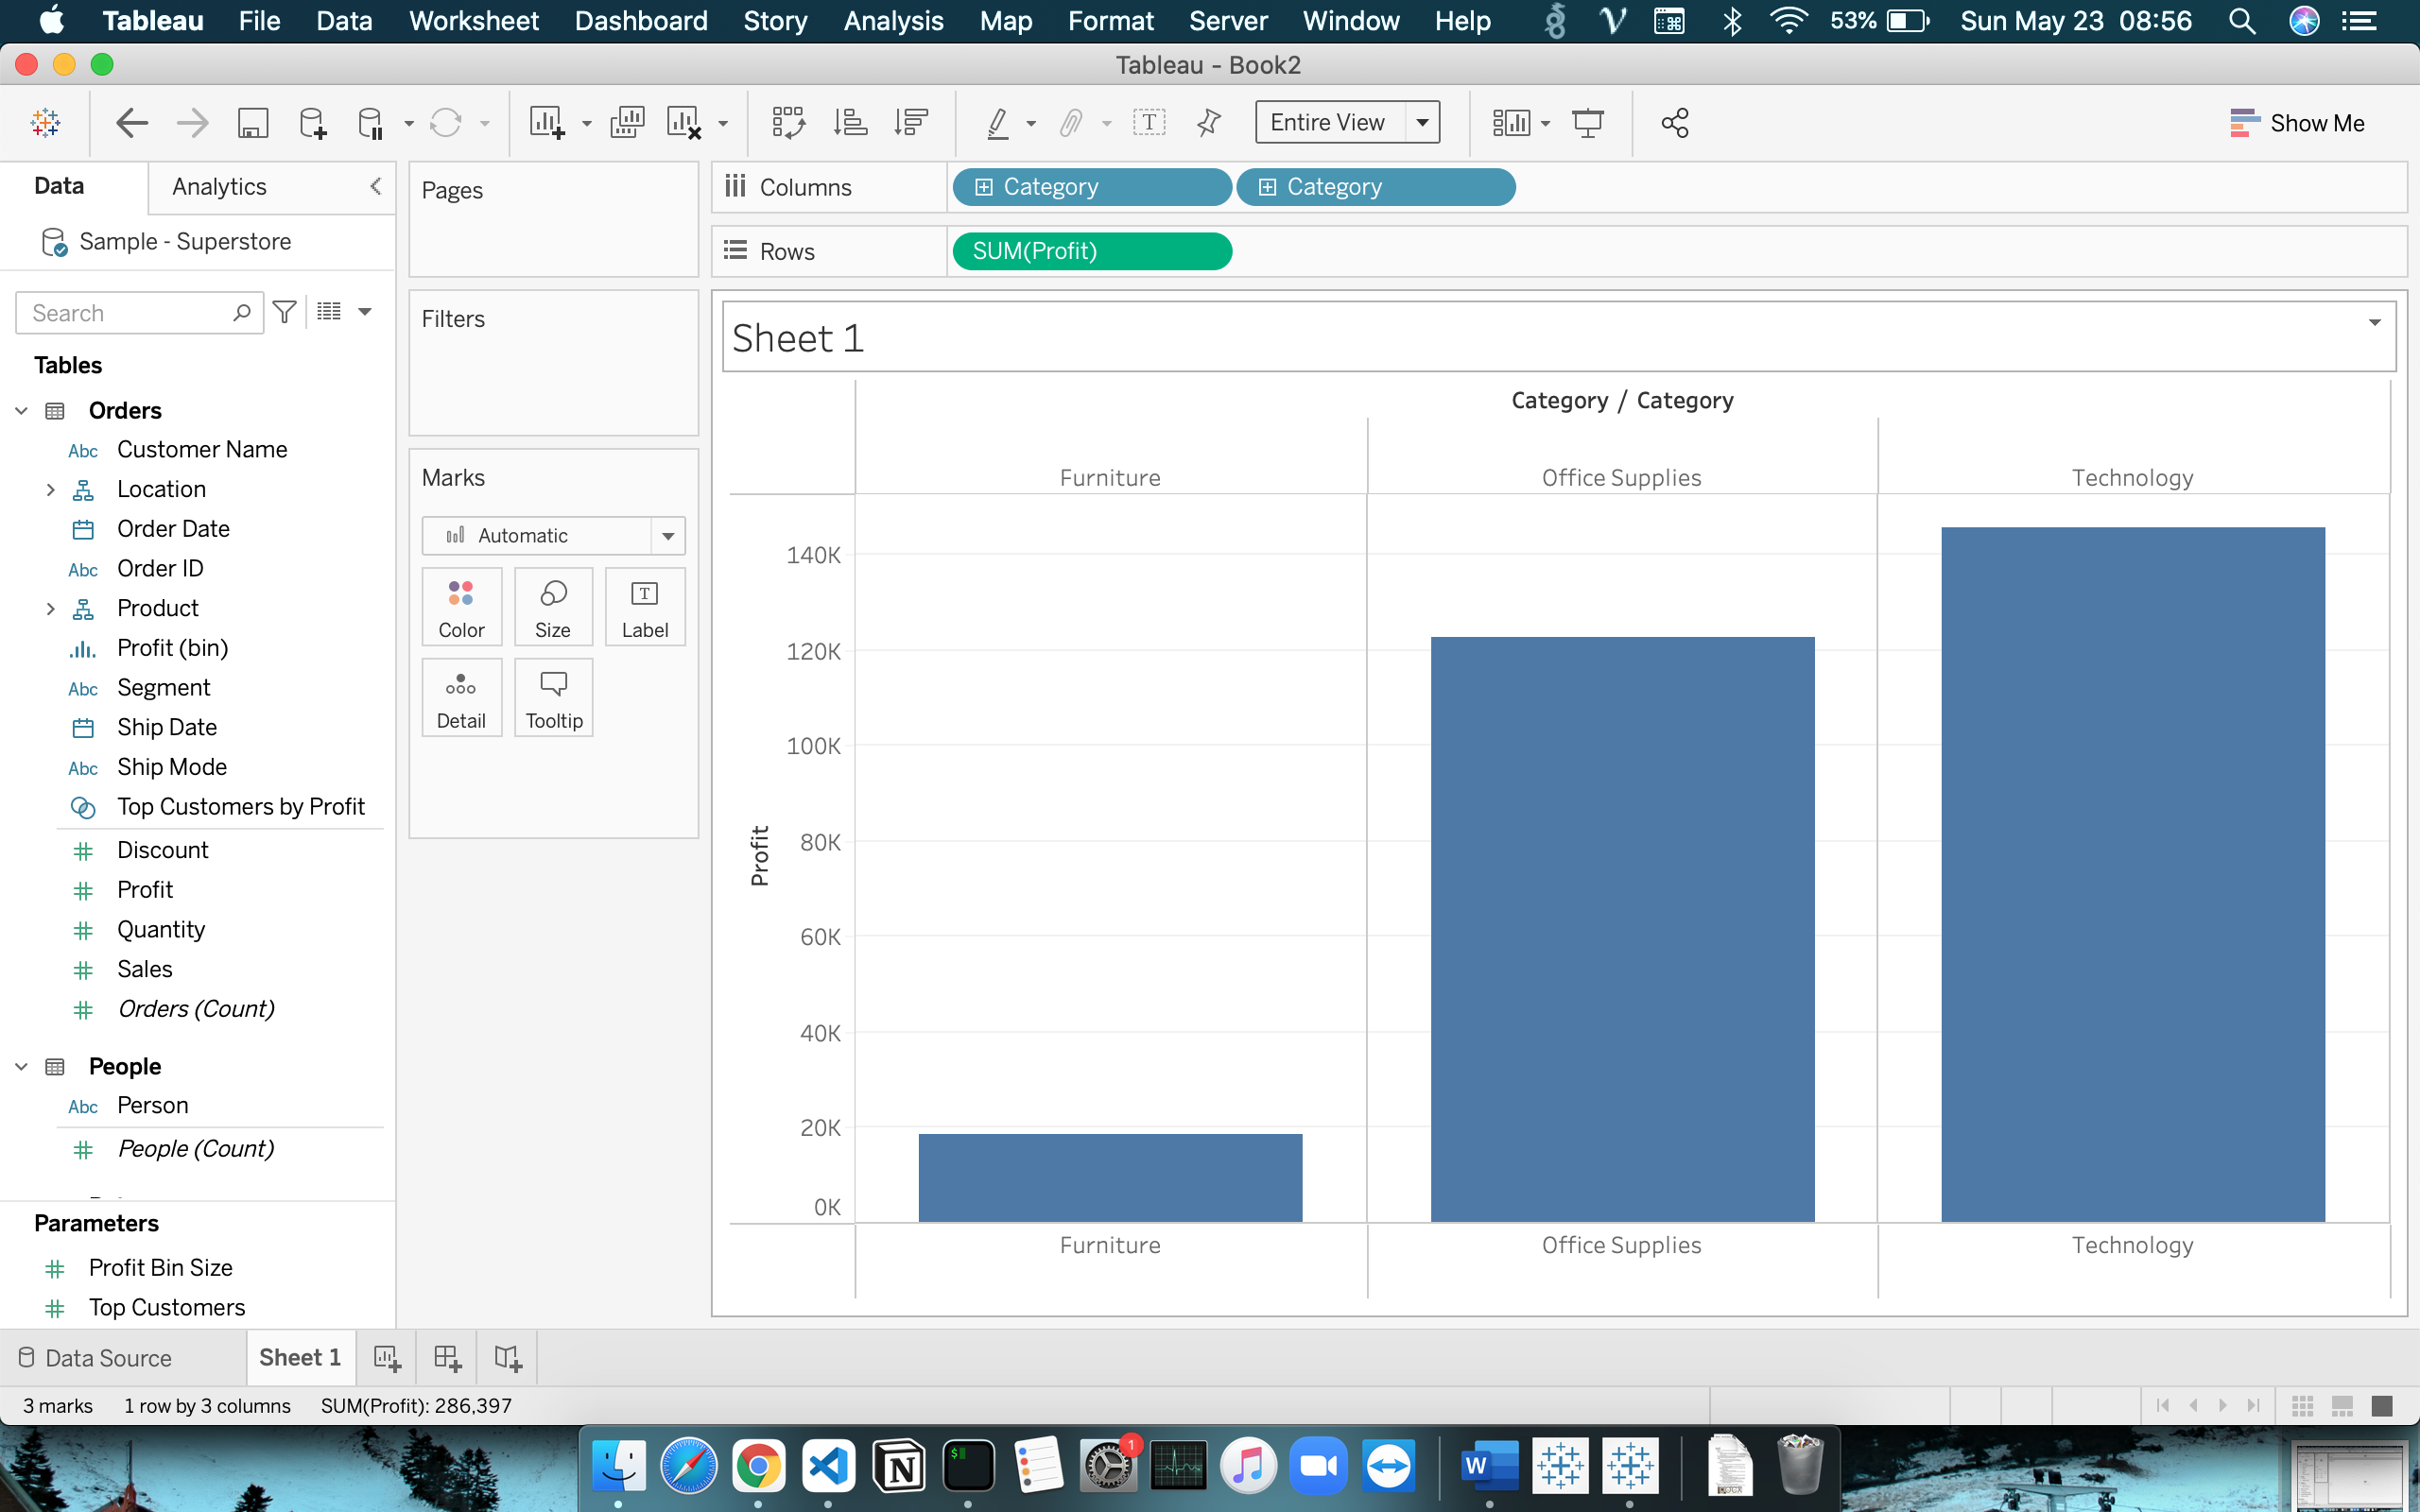
\includegraphics[scale=0.3]{img/barChart.png}
            \caption{Biểu đồ thể hiện lợi nhuận của mỗi loại sản phẩm}
        \end{center}
    \end{figure}

    \begin{itemize}
        % \item Để thực hiện loại biểu đồ này, ta cần chuẩn bị dữ liệu bao gồm: ít nhất 0 chiều dữ liệu; ít nhất 1 độ đo (yêu cầu này có thể xem tại mục "Show Me", nơi đề xuất các loại biểu đồ có thể thực hiện)
        % \item Thực hiện kéo thả chiều dữ liệu "Product" và ô "Columns" trong khung chứa dữ liệu trực quan. Sau đó kéo thả "Profit" (measure) vào ô "Rows", ta thu được biểu đồ sau


        \item Các độ đo có thể được tùy chỉnh với các tùy chọn trong hình sau
        \begin{figure}[H]
            \begin{center}
                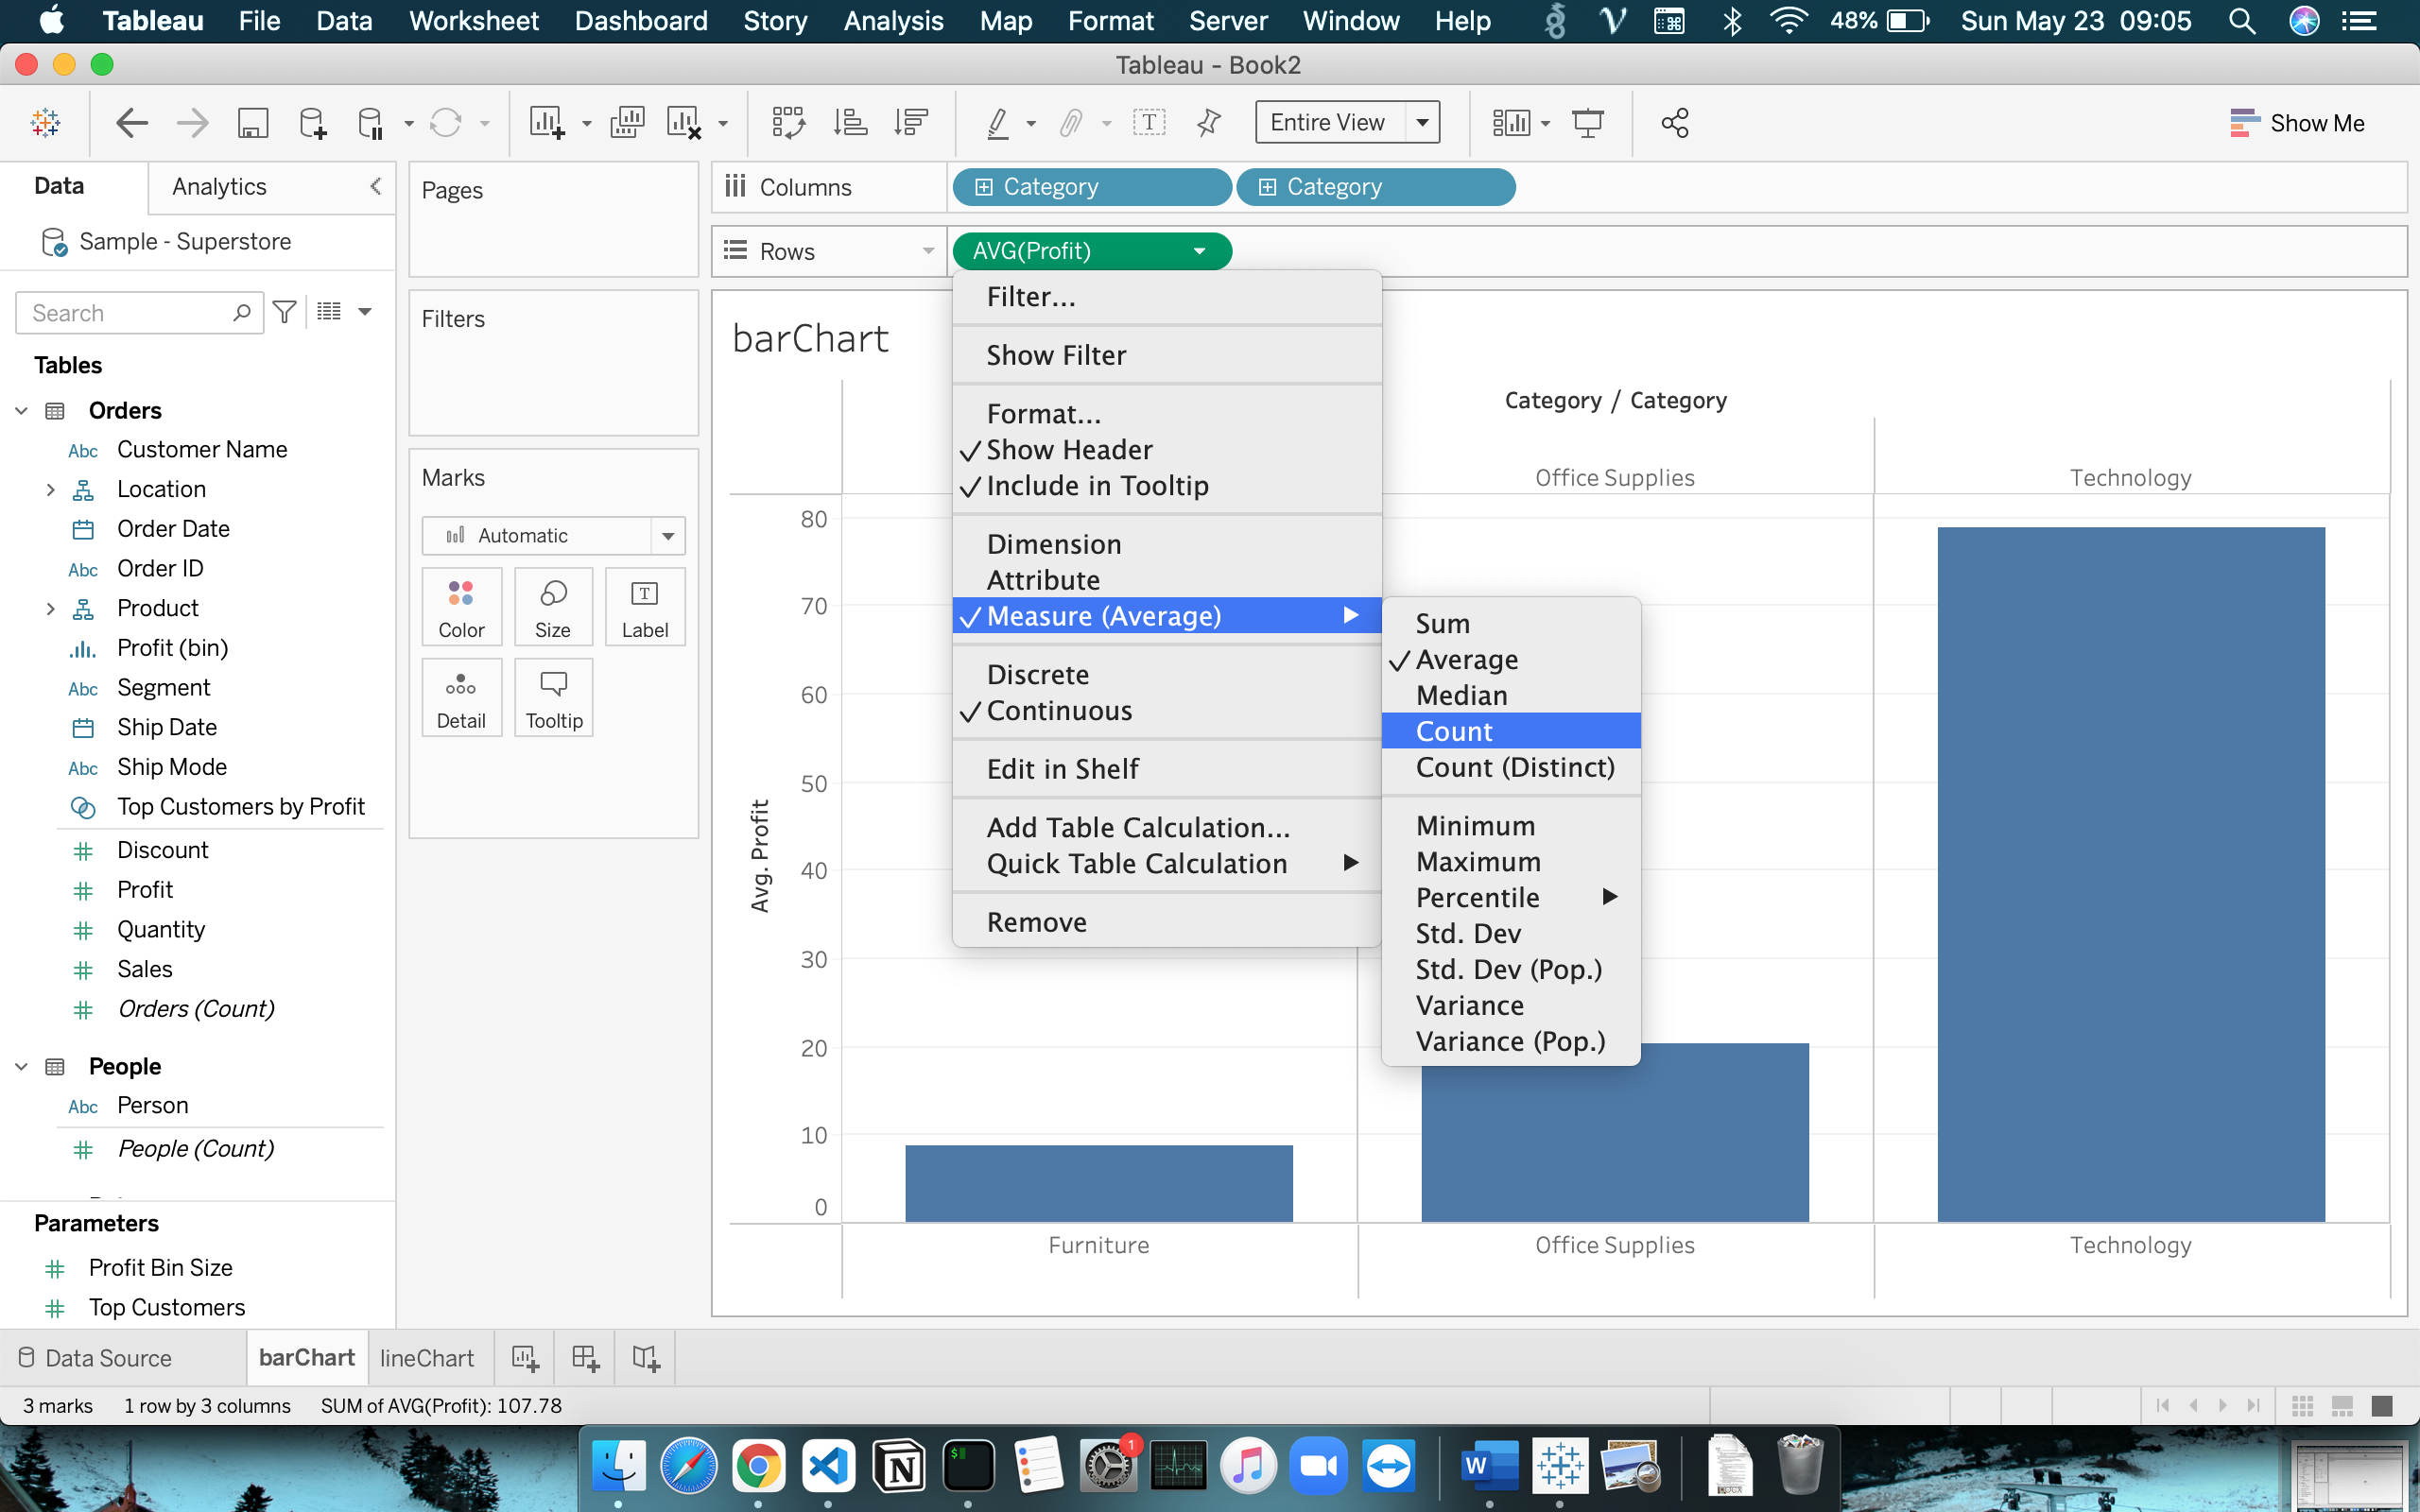
\includegraphics[scale=0.3]{img/measure.png}
                \caption{Các loại độ đo có thể chọn}
            \end{center}
        \end{figure}

        \item Ngoài ra, có thể điều chỉnh màu sắc, gắn thêm nhãn vào cột của biểu đồ. Các điều chỉnh này có thể áp dụng cho nhiều loại biểu đồ khác nhau nhưng phải thỏa mãn logic biểu diễn. Sau khi điều chỉnh, ta có thể thu được kết quả như sau
        % \begin{itemize}
        %     \item Kéo thả trường dữ liệu chứa nội dung cần phân loại bằng màu sắc vào ô "Color" của khung chứa bộ lọc và điều chỉnh dữ liệu để chọn màu
        %     \item Kéo thả trường dữ liệu chứa nội dung nhãn dán vào ô "Label" của khung chứa bộ lọc và điều chỉnh dữ liệu để chọn màu
        % \end{itemize}
        \begin{figure}[H]
            \begin{center}
                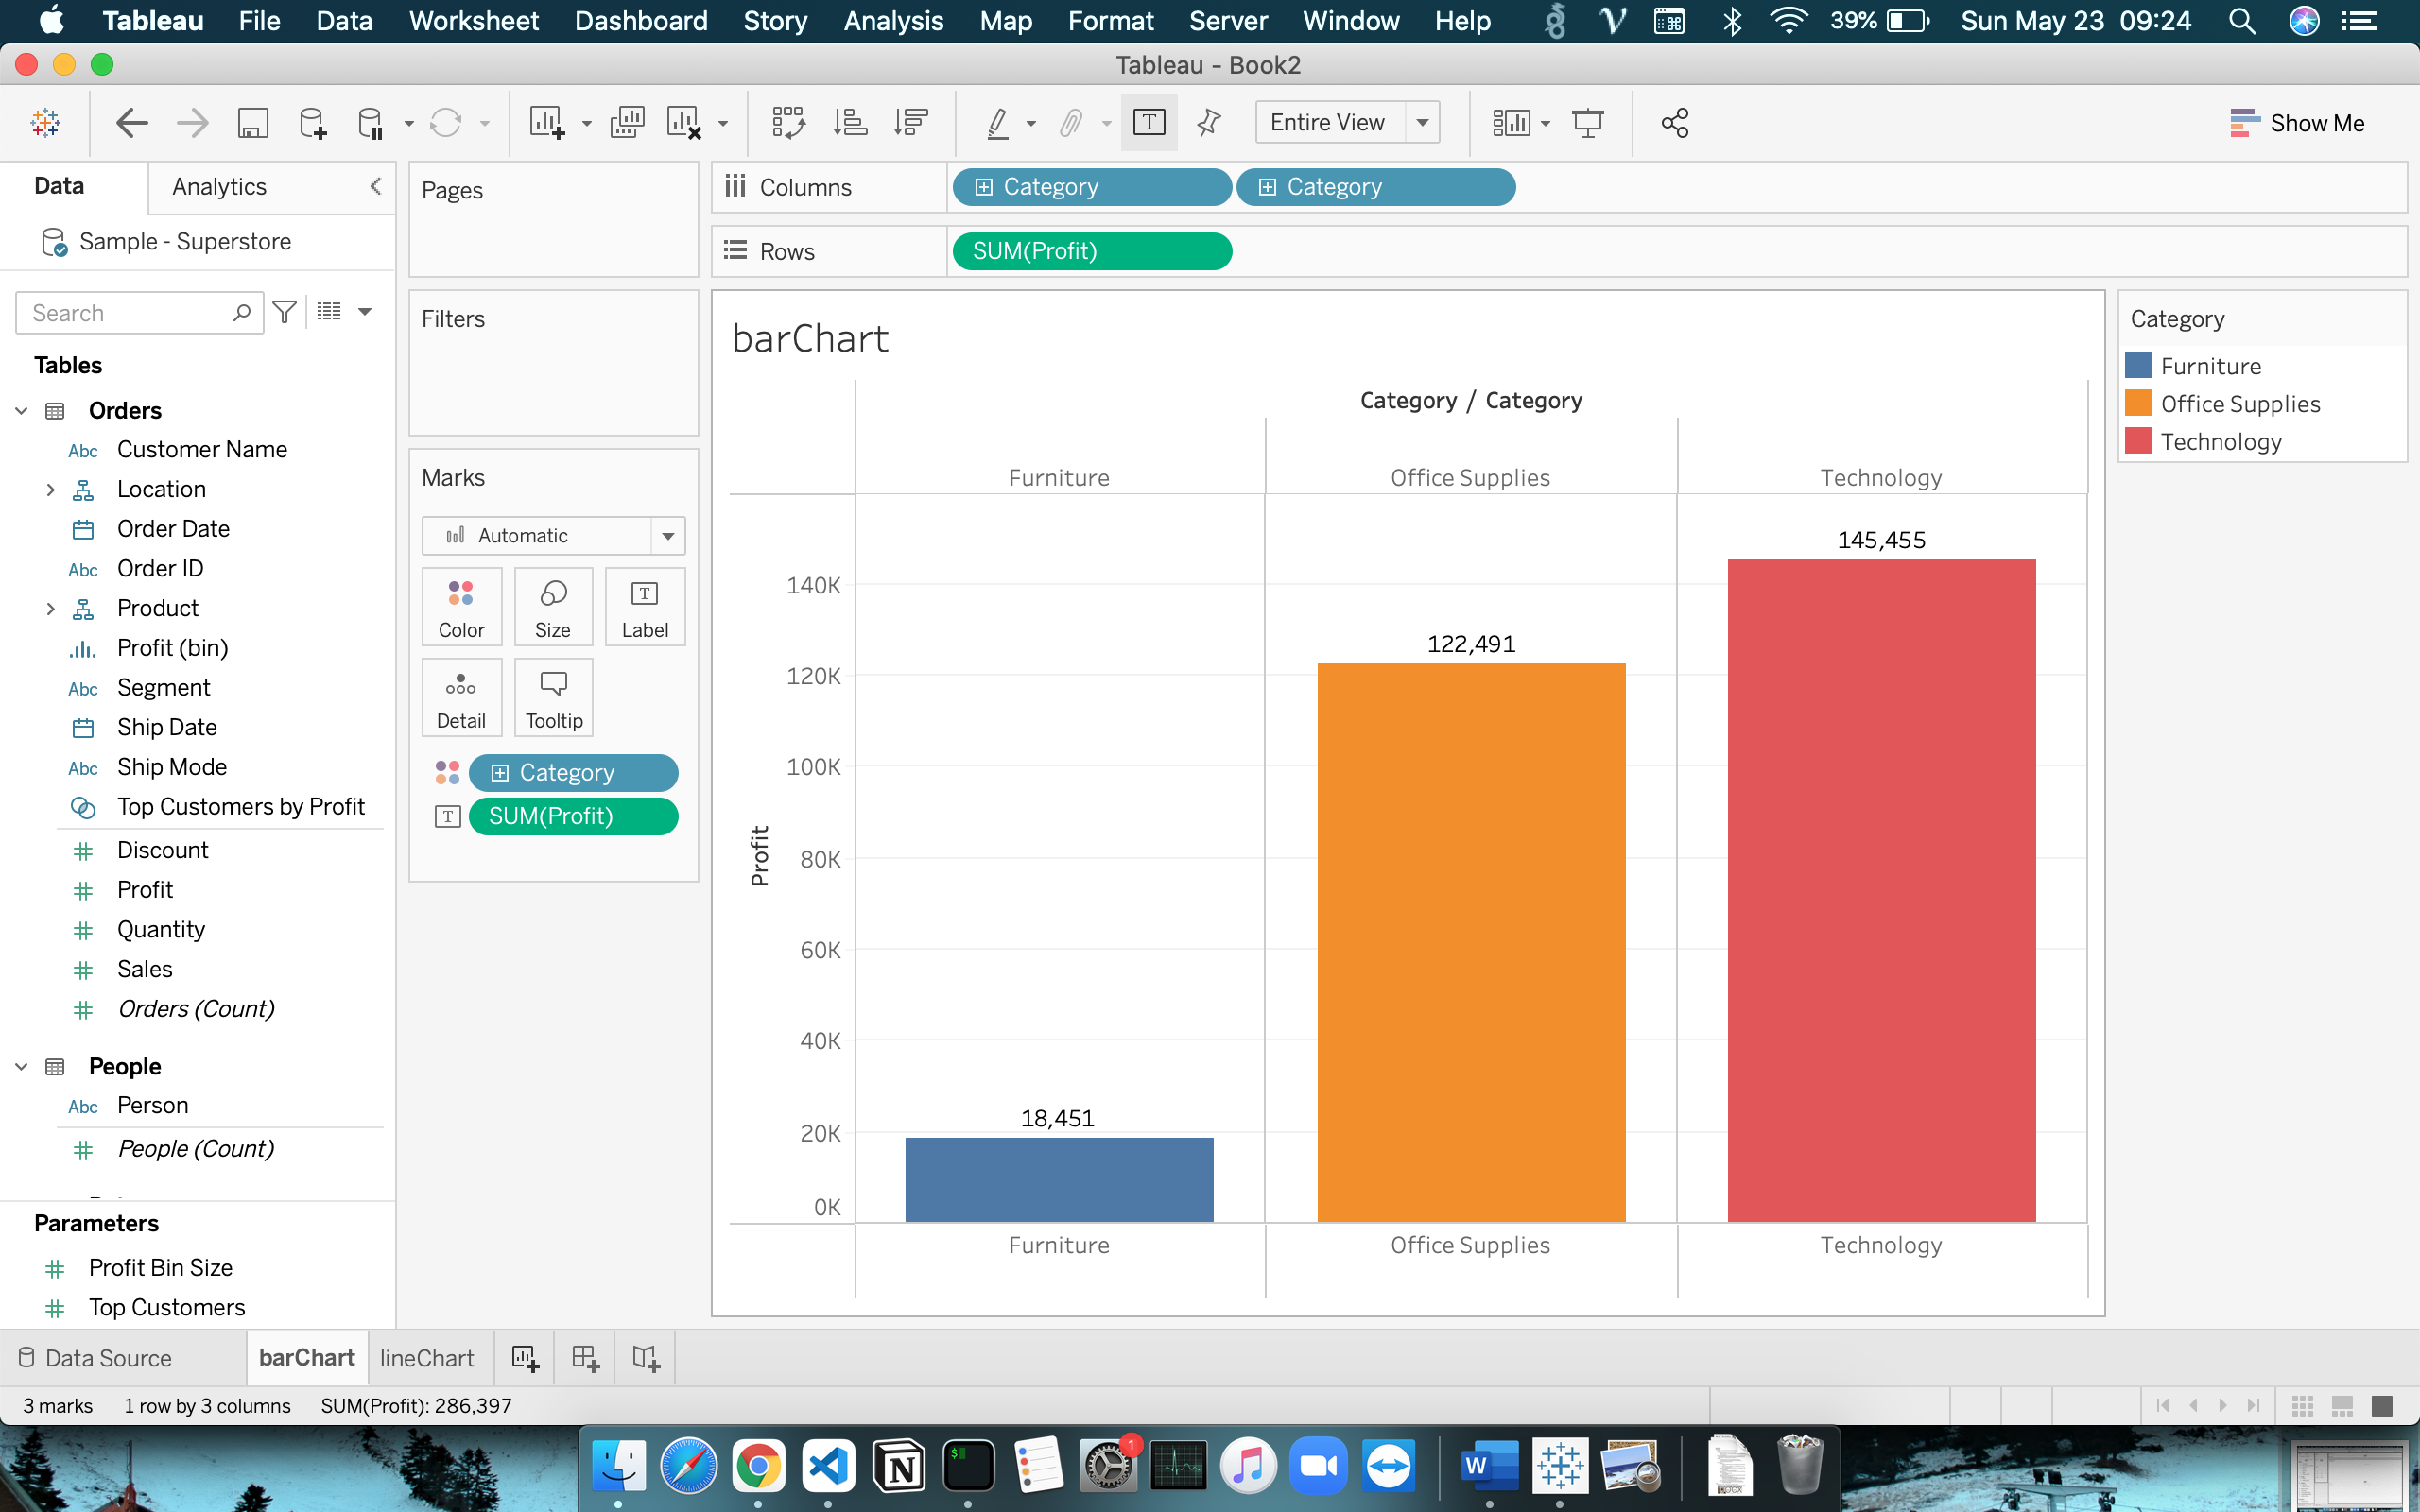
\includegraphics[scale=0.3]{img/barChart1.png}
                \caption{Gắn nhãn và biểu diễn dữ liệu bằng màu sắc}
            \end{center}
        \end{figure}
    \end{itemize}

    \item Biểu đồ đường: Loại biểu đồ thể hiện giá trị thực của dữ liệu. Thường được biểu diễn theo thời gian. Phục vụ so sánh, phân tích xu hướng theo thời gian,...
    \begin{figure}[H]
        \begin{center}
            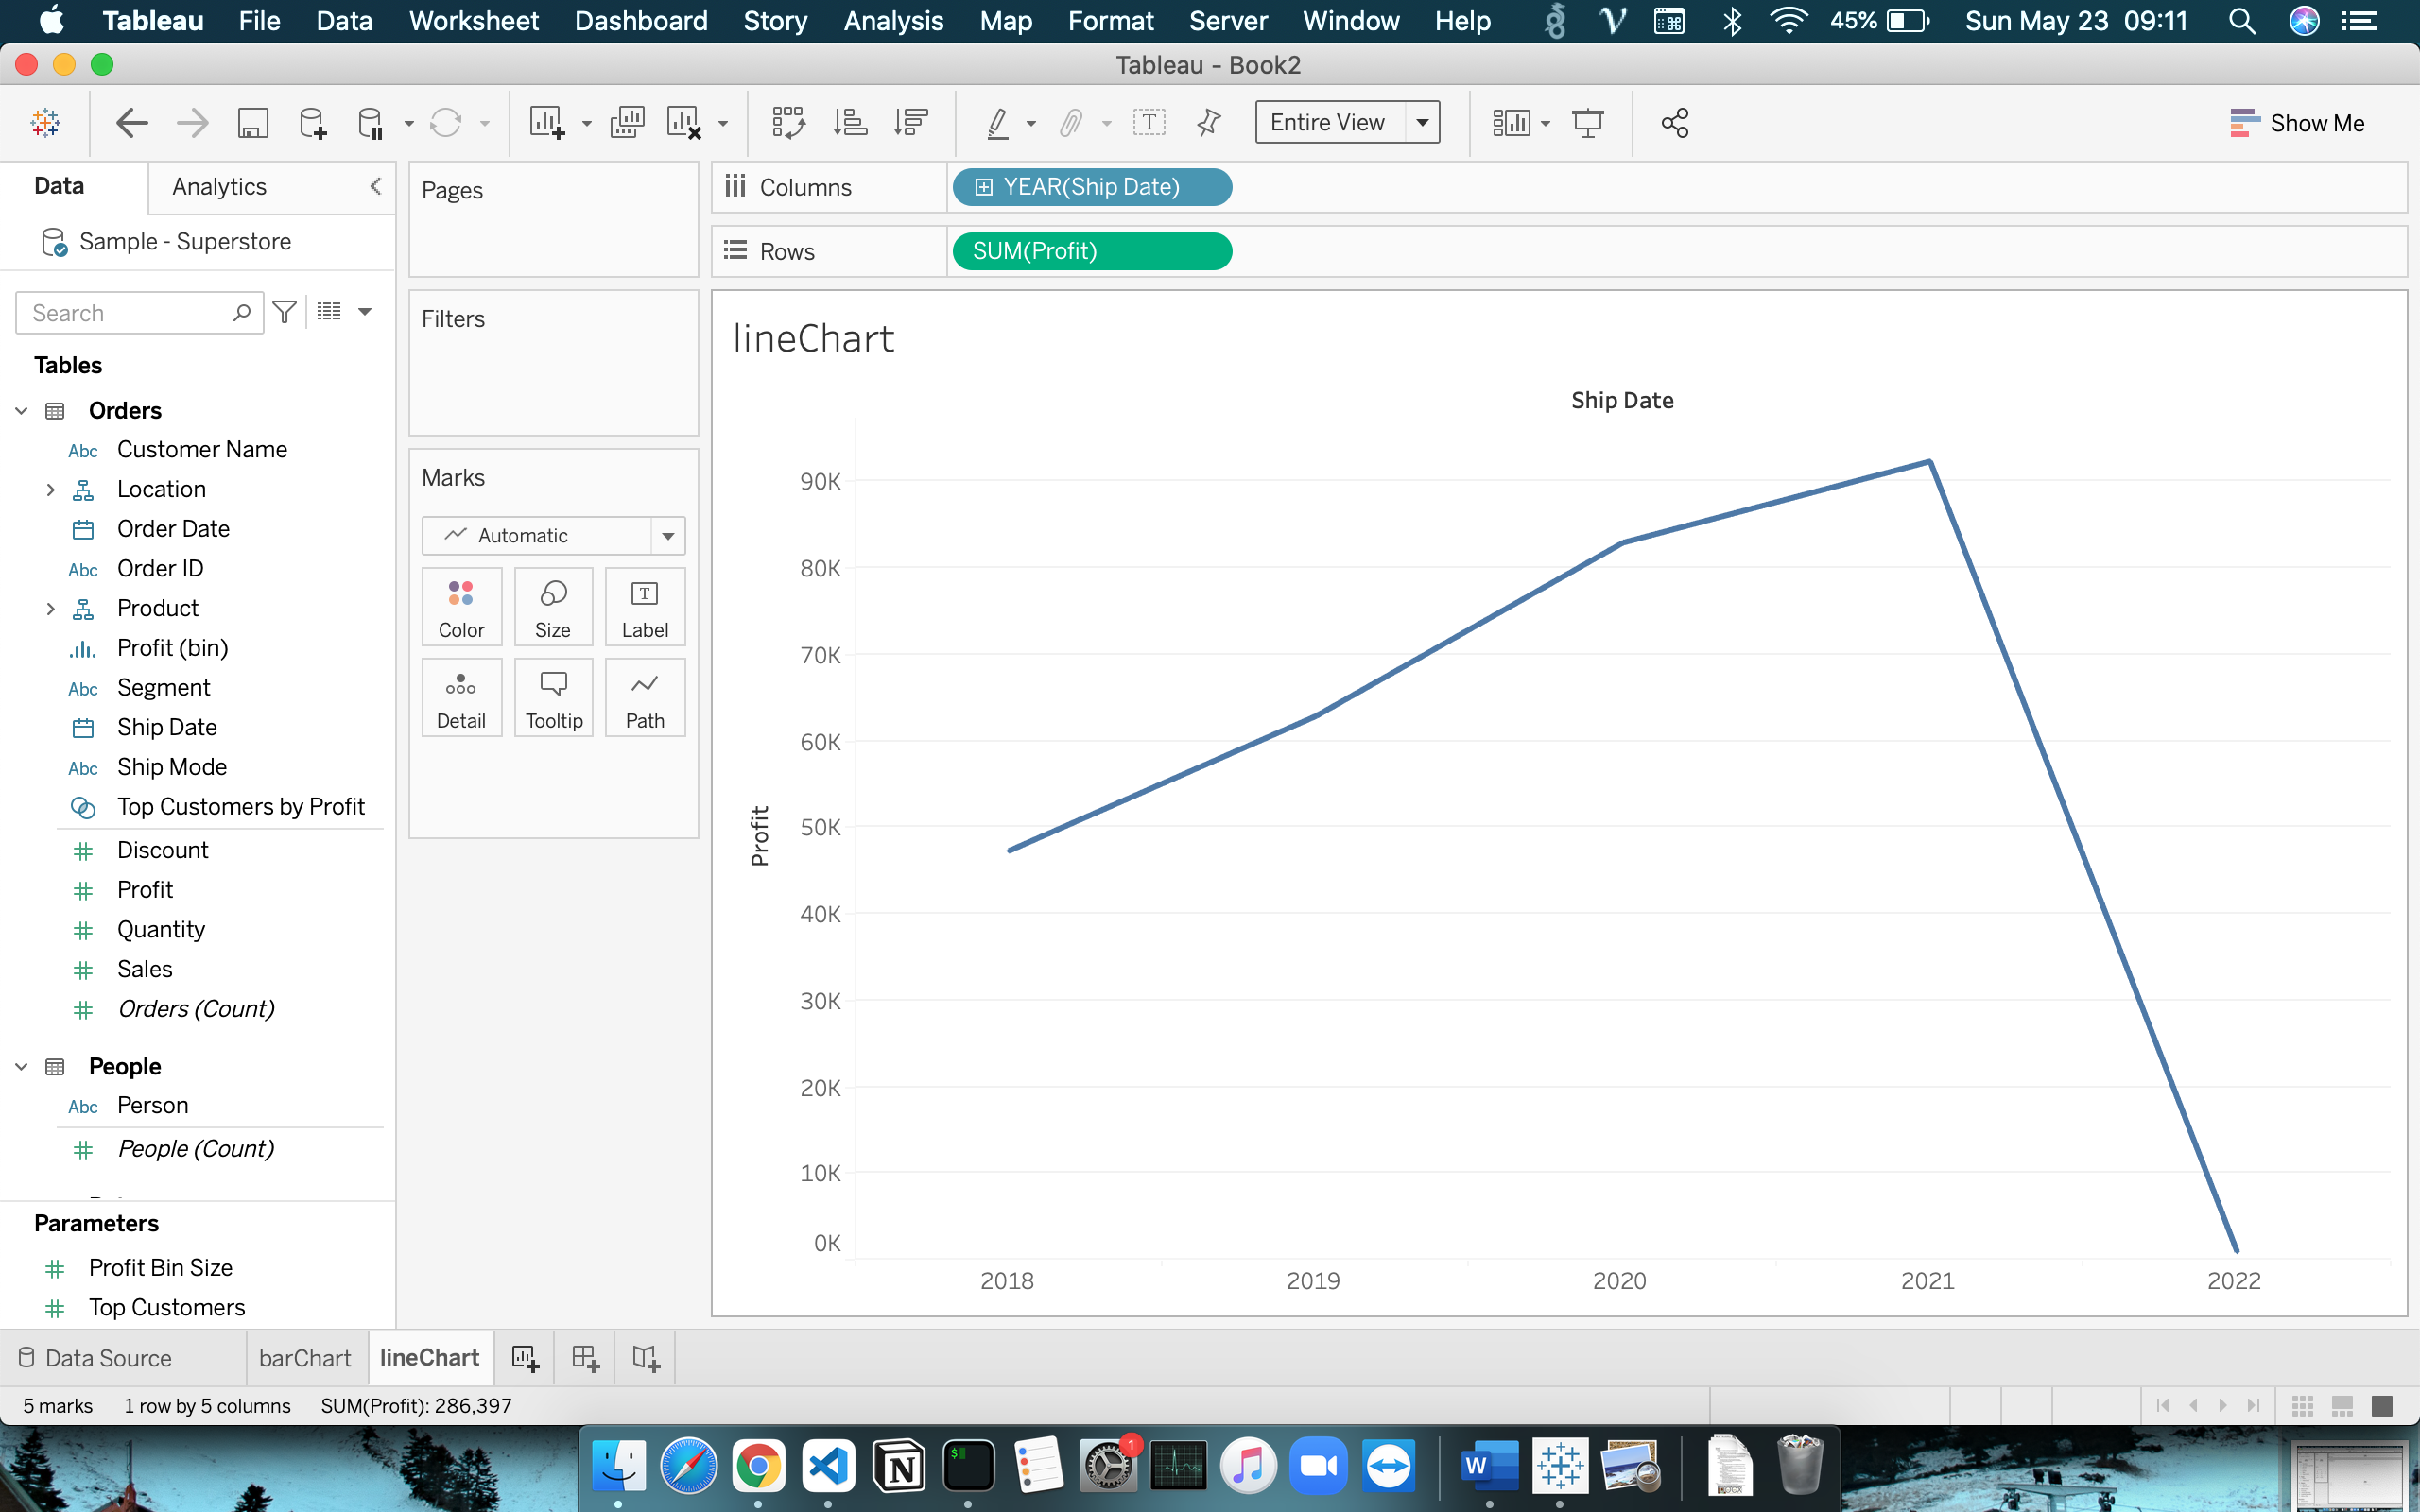
\includegraphics[scale=0.3]{img/lineChart.png}
            \caption{Biểu đồ thể hiện lợi nhuận công ty theo năm}
        \end{center}
    \end{figure}
    % \begin{itemize}
    %     \item Để thực hiện loại biểu đồ này, ta cần chuẩn bị dữ liệu bao gồm: 1 trường dữ liệu biểu diễn thời gian (có thể không cần), ít nhất 0 chiều dữ liệu, ít nhất 1 độ đo (yêu cầu này có thể xem tại mục "Show Me", nơi đề xuất các loại biểu đồ có thể thực hiện)
    %     \item Thực hiện kéo thả trường dữ liệu "YEAR" vào ô "Columns", "Profit" (measure) vào ô "Rows", ta thu được kết quả sau
    % \end{itemize}

    \item Kết hợp biểu đồ cột và biểu đồ đường
    \begin{figure}[H]
        \begin{center}
            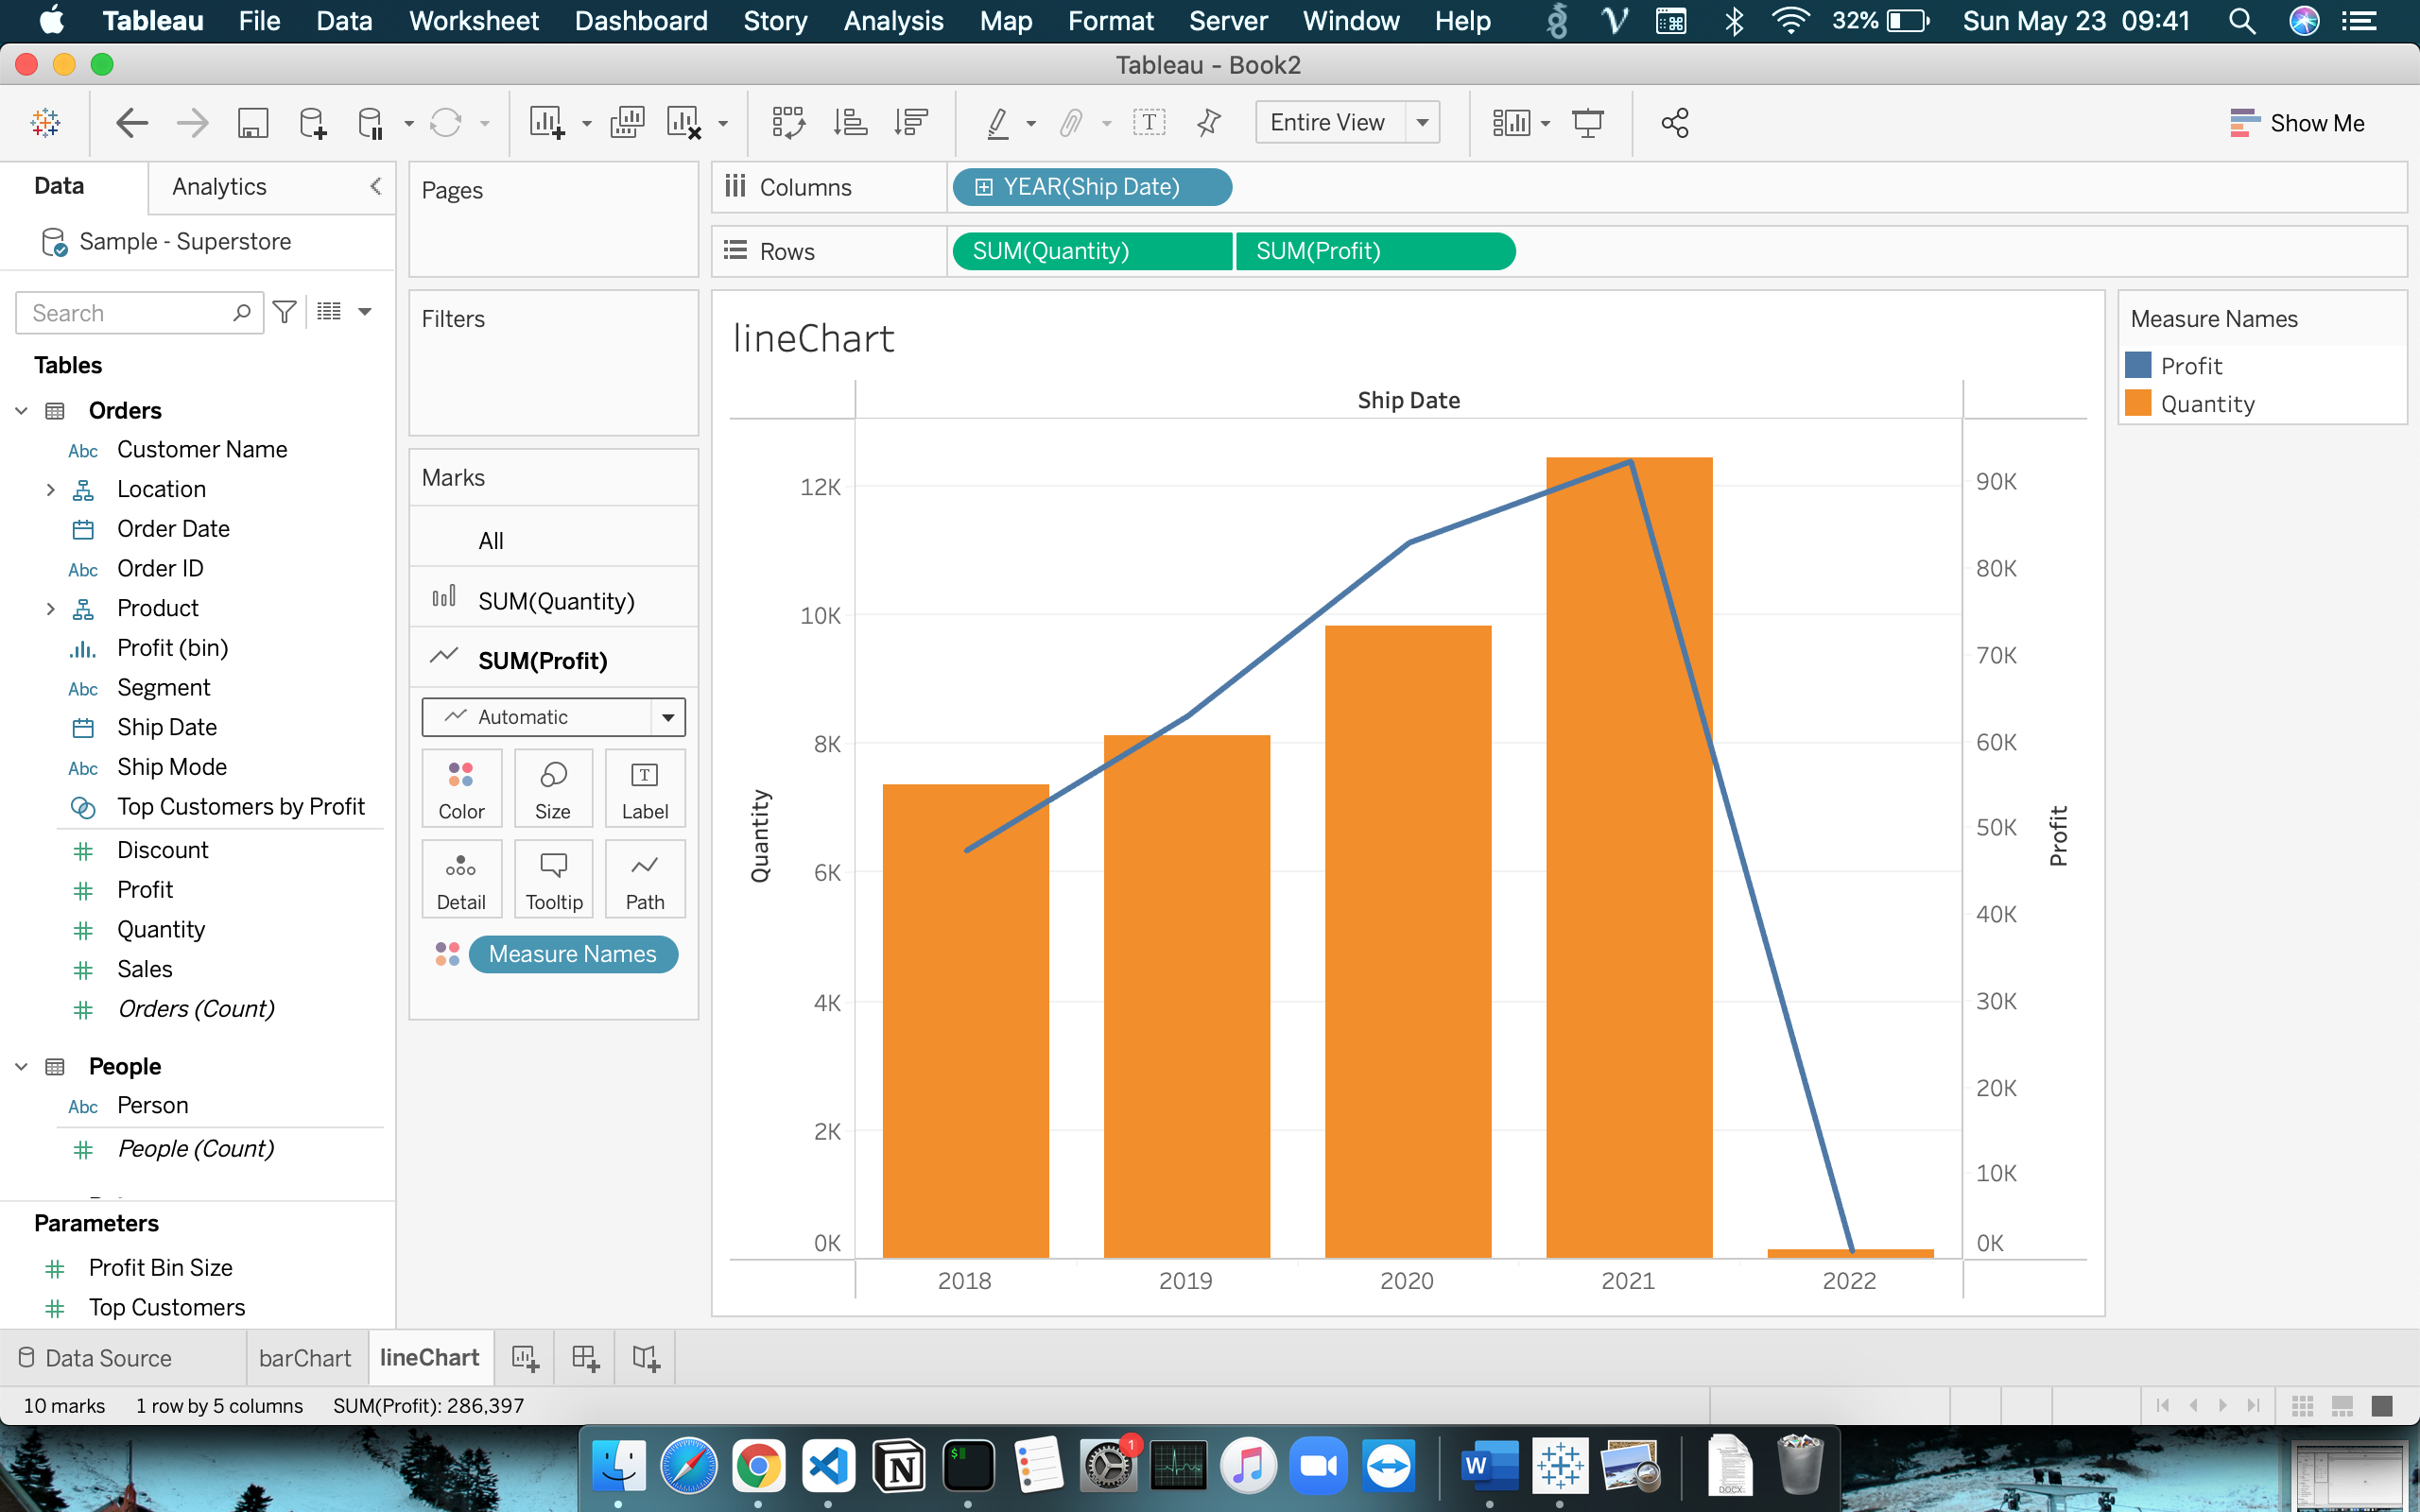
\includegraphics[scale=0.3]{img/lineBar.png}
            \caption{Biểu đồ thể hiện lợi nhuận và số lượng sản phẩm của công ty theo năm}
        \end{center}
    \end{figure}

    \item Biểu diễn bản đồ dựa trên địa danh hoặc tọa độ địa lý
    \begin{itemize}
        \item Sử dụng nhiều bộ lọc để trực quan top 10 bang có doanh thu cao nhất
        \begin{itemize}
            \item Kích thước: Biểu diễn tổng số doanh thu 
            \item Màu sắc: Biểu diễn tên bang 
            \item "Detail": Được dùng để xác định vị trí các bang theo tên
        \end{itemize}

        \item Kết quả thu được
        \begin{figure}[H]
            \begin{center}
                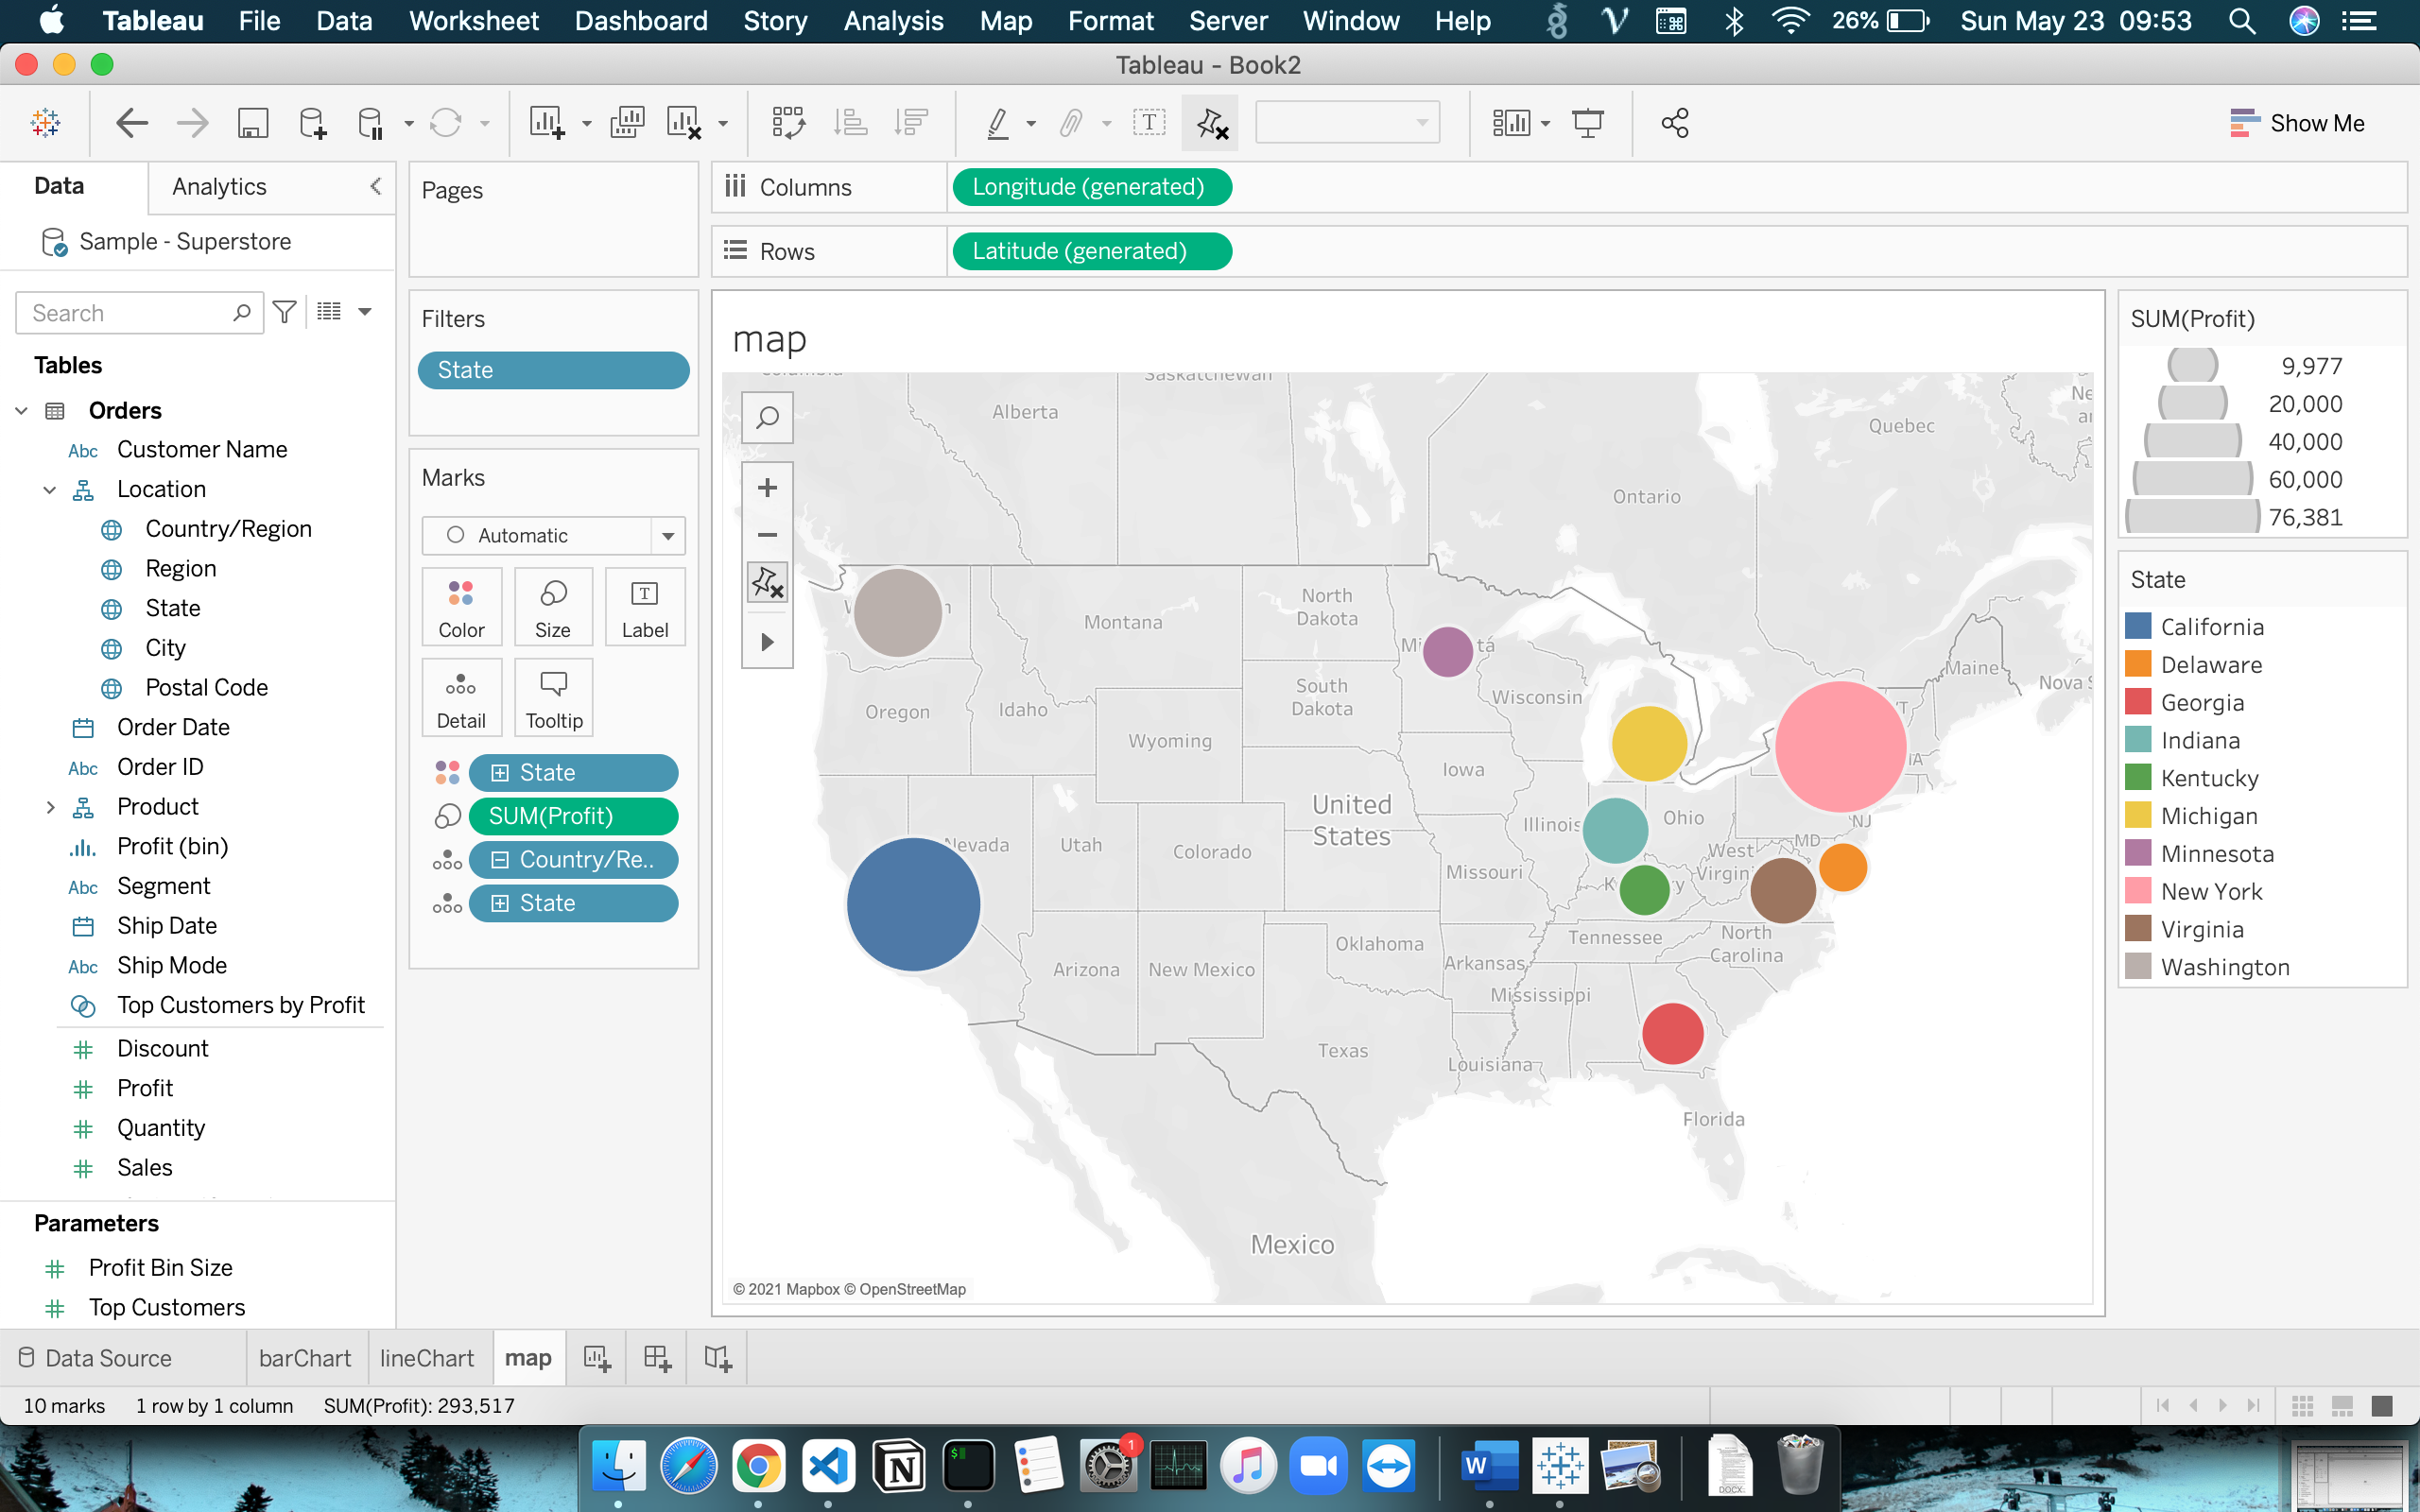
\includegraphics[scale=0.4]{img/map.png}
                \caption{Biểu đồ thể hiện top 10 bang có lợi nhuận cao nhất}
            \end{center}
        \end{figure}
    \end{itemize}
\end{itemize}

\subsubsection{Dashboard \& Story}

\begin{itemize}
    \item Dashboard 
    \begin{itemize}
        \item Tableau Dashboard cung cấp một cái nhìn toàn diện về dữ liệu doanh nghiệp bằng cách tổng hợp lại các biểu đồ đã vẽ trong các sheet
        \item Tableau Dashboard cung cấp nhiều thông tin hữu dụng nhờ tính năng biểu diễn dữ liệu theo định dạng trình tự thời gian, cho phép bổ sung nhiều chế độ xem và đối tượng, cung cấp nhiều loại bố cục và định dạng, cho phép doanh nghiệp triển khai các bộ lọc phù hợp
        \item Minh họa Dashboard
        \begin{figure}[H]
            \begin{center}
                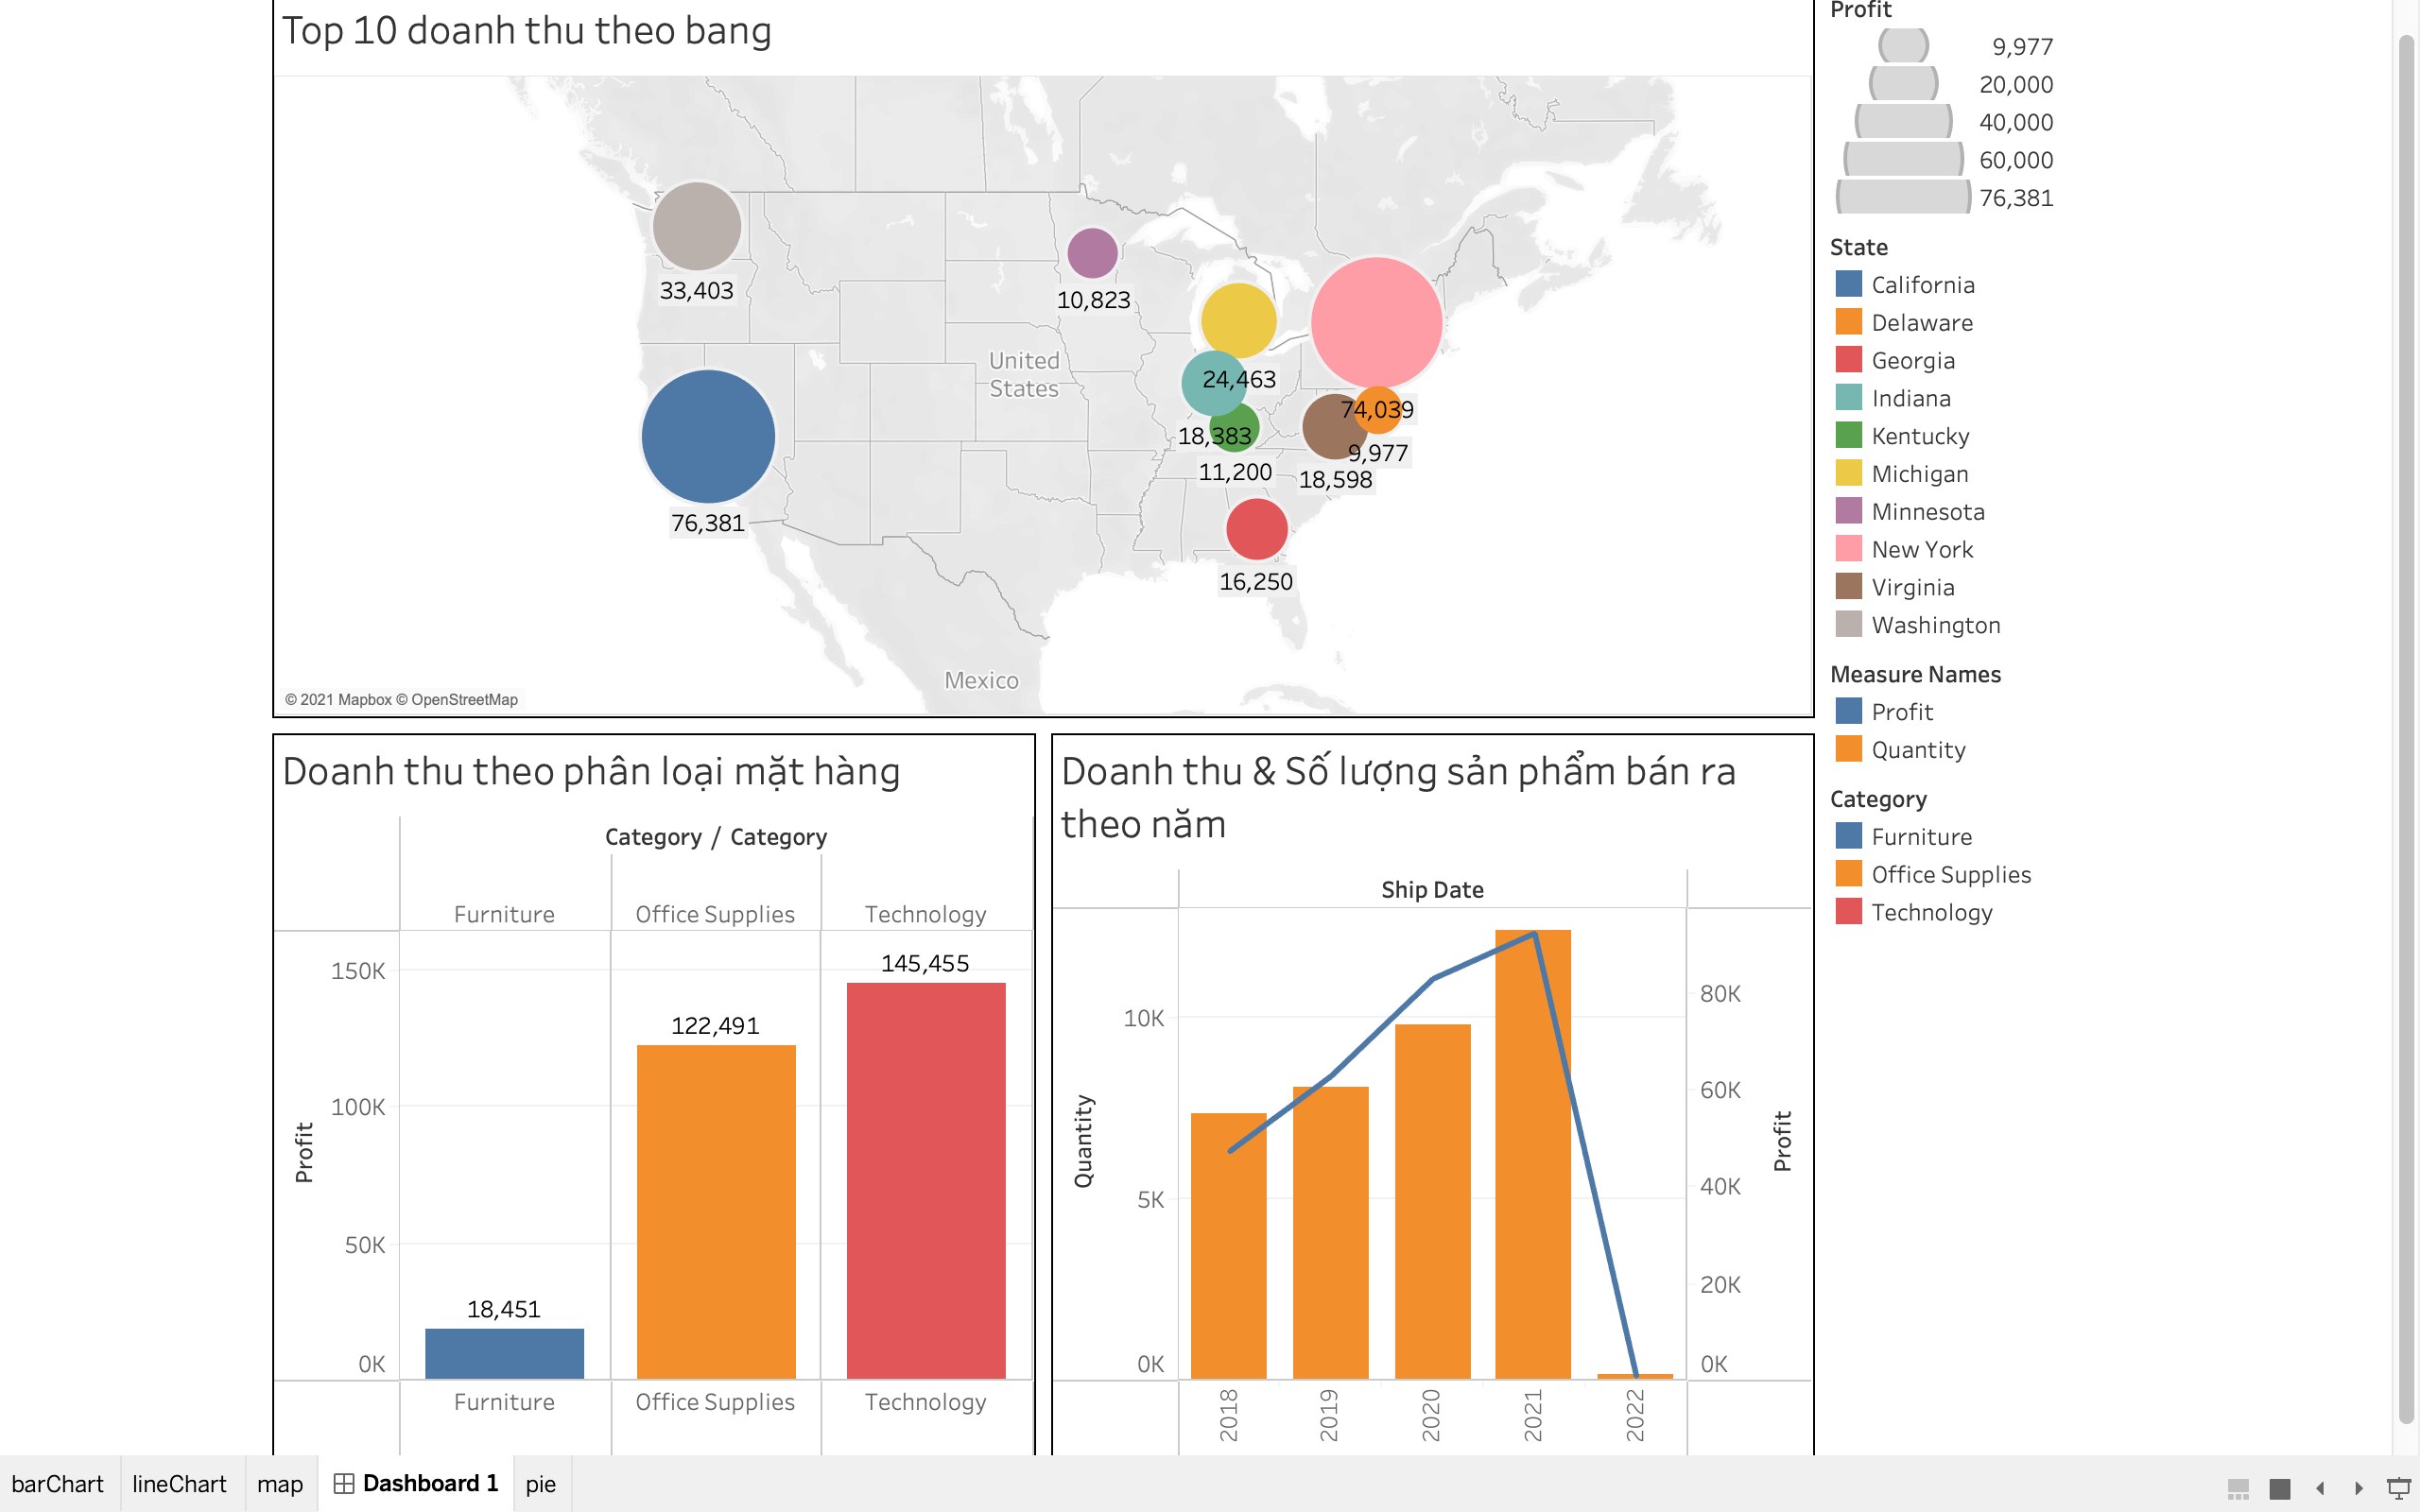
\includegraphics[scale=0.3]{img/dashboard.png}
                \caption{Dashboard tổng hợp các biểu đồ vừa vẽ}
            \end{center}
        \end{figure}
    \end{itemize}

    \item Story
    \begin{itemize}
        \item Story là một chuỗi các hình ảnh phối hợp với nhau để truyền tải một thông điệp, một câu chuyện
        \item Ta có thể tạo các story để kể một câu chuyện dữ liệu, cung cấp bối cảnh, chứng minh các quyết định liên quan đến kết quả như thế nào, hoặc đưa ra một trường hợp thuyết phục
    \end{itemize}
\end{itemize}

\subsubsection{Các tính năng khác}

\begin{itemize}
    \item Nhập dữ liệu với kích thước lớn, quản lý siêu dữ liệu
    \item Hỗ trợ tạo các truy vấn bằng thao tác đơn giản
    \item Phân tích dữ liệu với BigData
    \item Phân tích theo thời gian chia sẻ, kết nối thông qua các ứng dụng trực tuyến thời gian thực
\end{itemize}

\clearpage

\section{Trực quan hóa dữ liệu Worldometer}

\begin{itemize}
    \item Với ý tưởng trực quan dữ liệu sử dụng đa biểu đồ, người viết hướng đến
    \begin{itemize}
        \item Ôn tập và bổ sung kiến thức về các dạng biểu đồ và các trường hợp sử dụng
        \item Từ nhiều góc nhìn, rút trích các thông tin có ích từ dữ liệu trực quan
    \end{itemize}

    \item Dữ liệu covid19 được thu thập từ ngày 14/04/2021 đến hết ngày 24/04/2021 với cách thu thập đã được báo cáo chi tiết trong Lab01
    \item Các biểu diễn dưới đây, hoặc sự dụng dữ liệu của ngày mới nhất trong tập dữ liệu (24/04/2021), hoặc biểu diễn chung cho tất cả các tập dữ liệu (từ ngày 14/04/2021 đến 24/04/2021)
\end{itemize}

\subsection{Biểu diễn Tree Map}

\begin{itemize}
    \item Lợi ích: Tree Map cho phép biểu diễn tập dữ liệu được sắp xếp theo thứ bậc. Mục đích là để chia nhỏ tập dữ liệu thành các phần cấu thành nó và nhanh chóng xác định các thành phần lớn hơn và nhỏ hơn của tập dữ liệu
    \item Biểu đồ cho một cái nhìn trực quan về tập dữ liệu của biến Total Cases, các giá trị của biến Total Cases của các nước thể hiện ít hay nhiều dựa theo kích thước của các hình chữ nhật
    \item Dễ dàng nhận thấy USA là nước có tổng số ca Covid nhiều nhất trên thế giới (hình chữ nhật lớn nhất) và tiếp sau đó là các nước India, Brazil, France...
    \begin{figure}[H]
        \begin{center}
            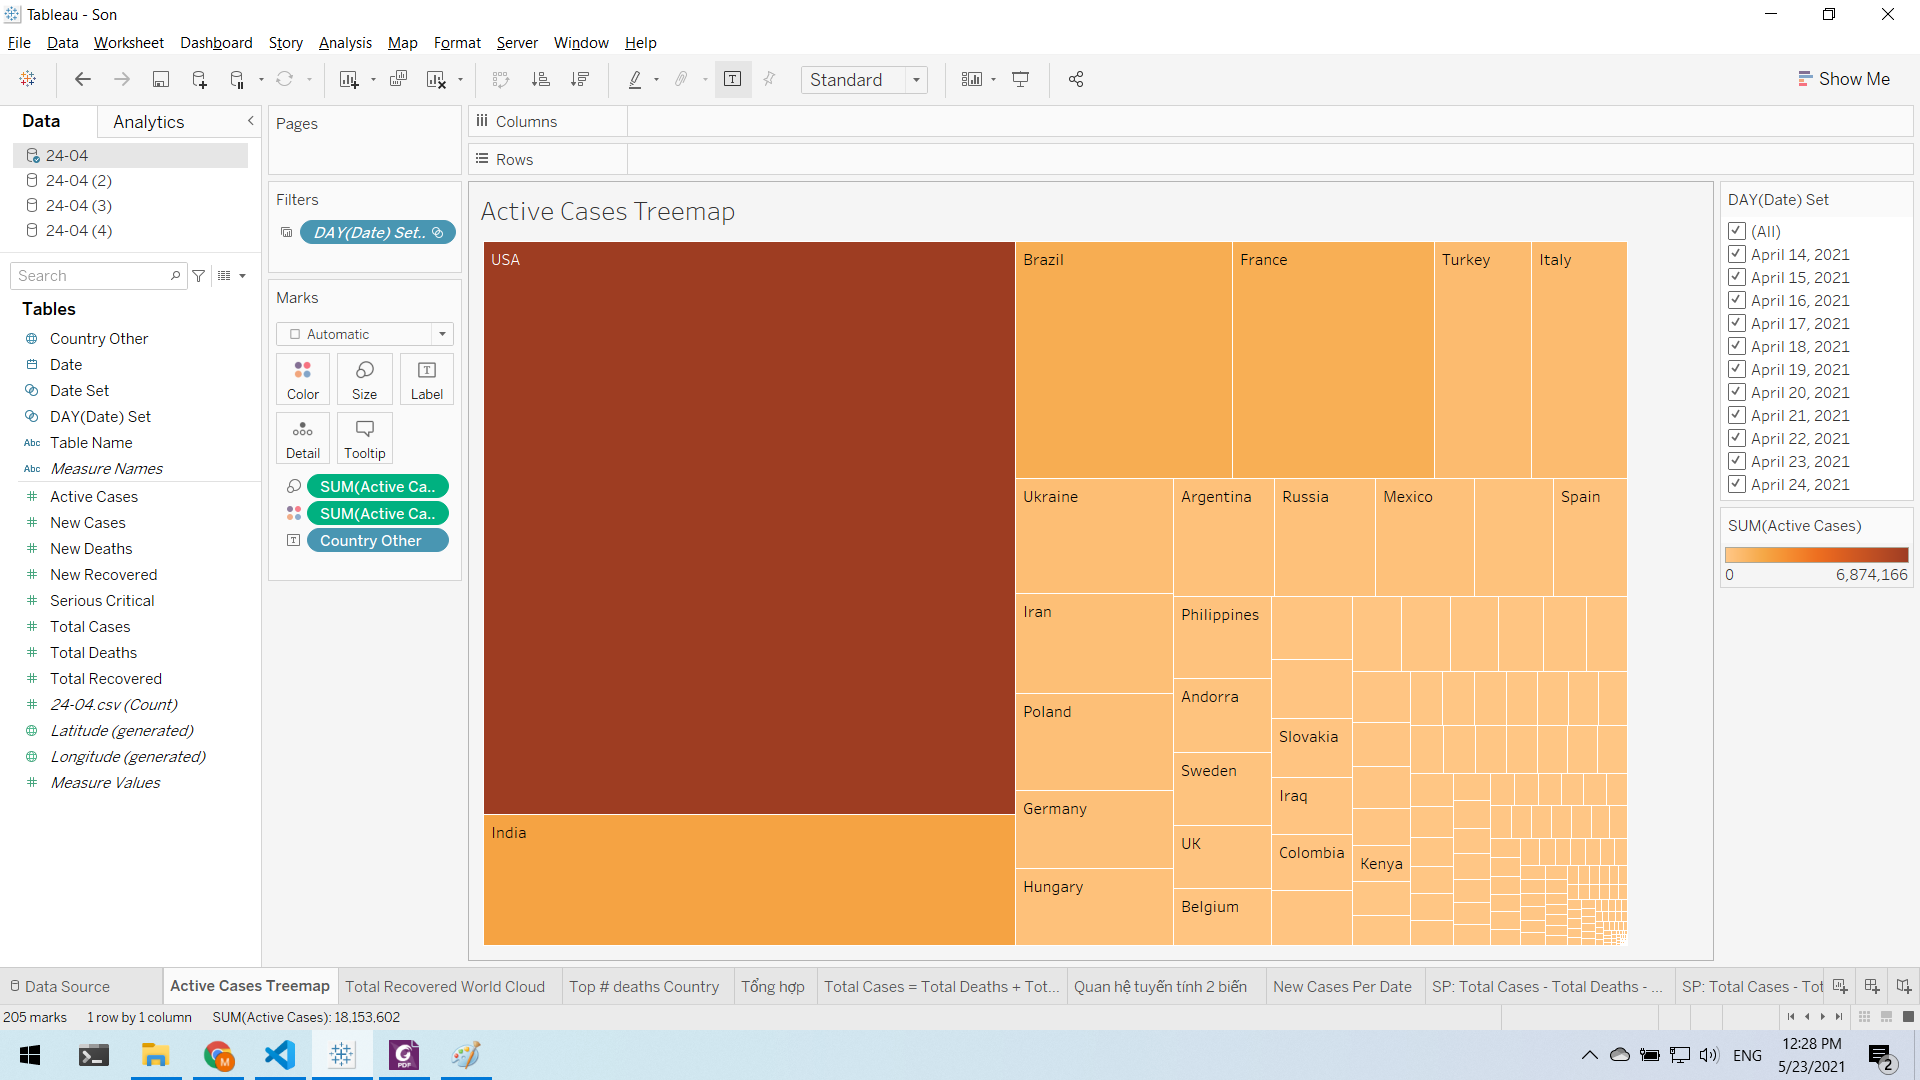
\includegraphics[scale=0.4]{img/treeMap.png}
            \caption{Biểu đồ biểu diễn xếp hạng số lượng ca nhiễm theo từng quốc gia}
        \end{center}
    \end{figure}
\end{itemize}

\subsection{Biểu diễn Word Cloud}

\begin{itemize}
    \item Lợi ích: Tương tự như Tree Map, Word Cloud cho phép người đọc dễ dàng nhận ra xu hướng dựa theo kích thước chữ, chữ càng lớn thì xu hướng càng nhiều, xu hướng nhiều nhất thường được để ở trung tâm của Cloud. Ngoài ra, loại biểu diễn này còn rất sinh động, tạo hứng thú cho người đọc
    \item Biểu đồ dễ dàng thể hiện được giá trị Total Cases của các nước. Trong đó, giá trị lớn nhất thuộc về USA (kích thước chữ lớn nhất, nằm ở trung tâm). Ngoài ra, ta cũng dễ dàng nhận thấy các nước có giá trị lớn tiếp theo dựa theo kích thước chữ
    \begin{figure}[H]
        \begin{center}
            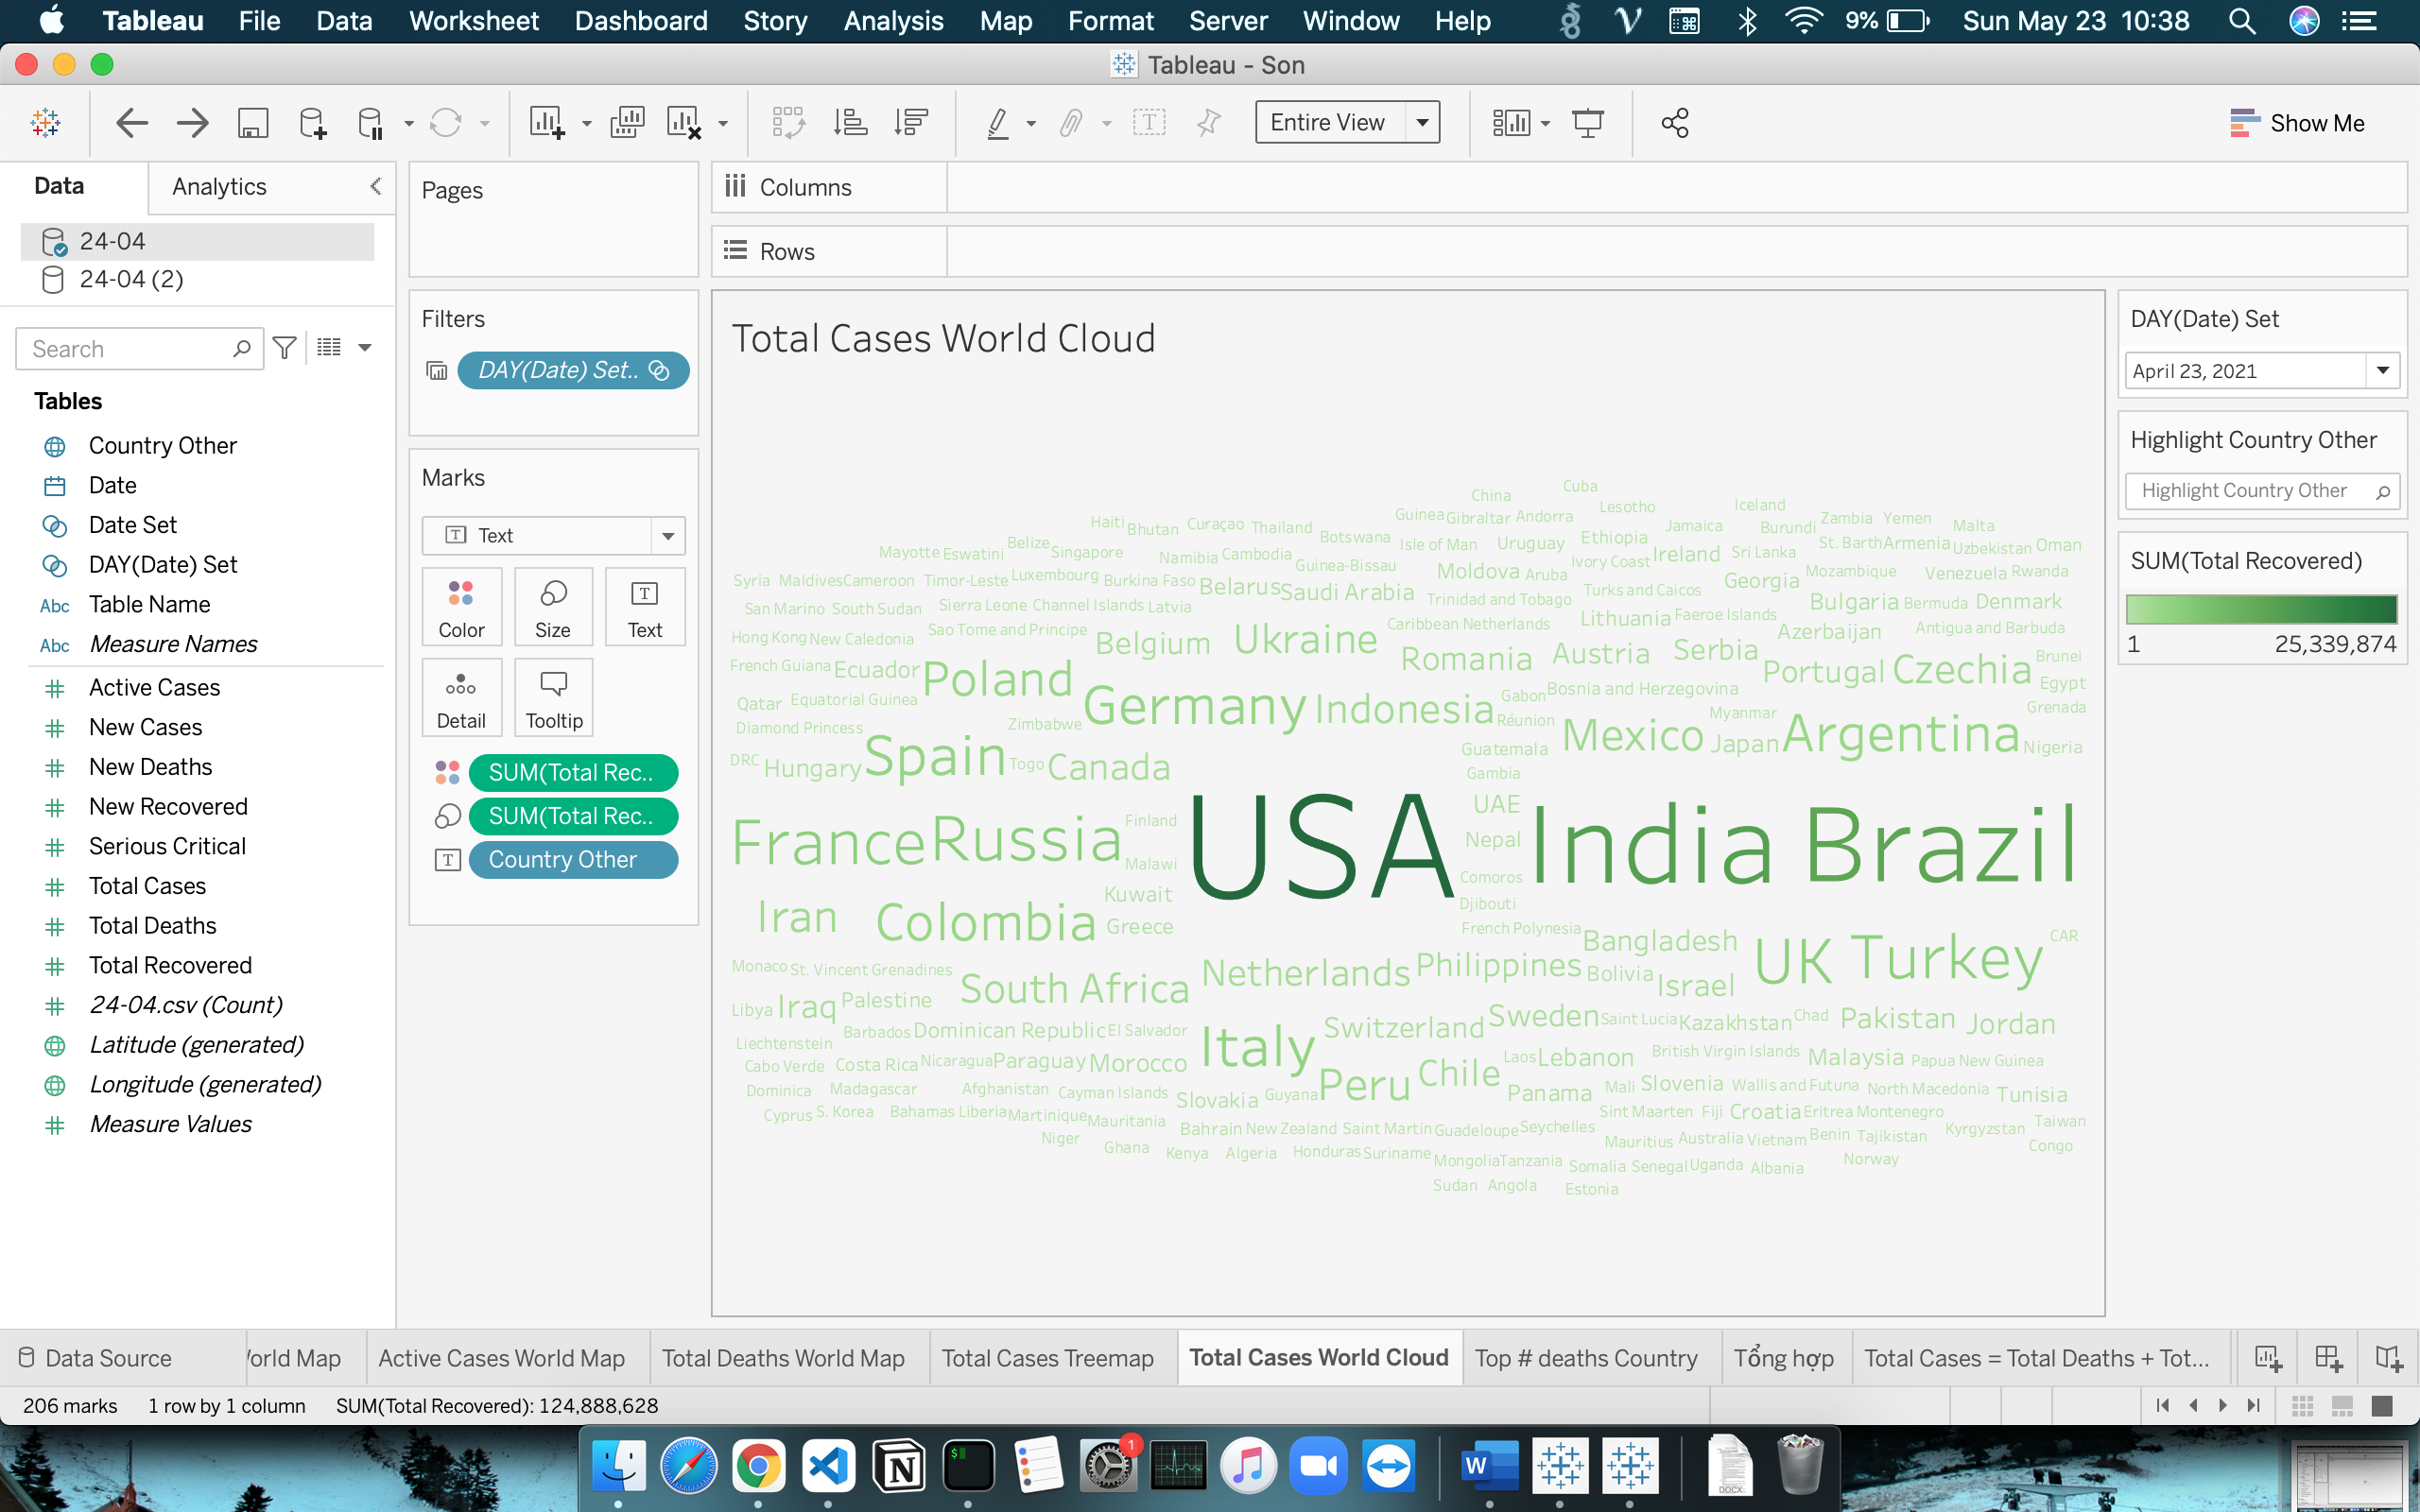
\includegraphics[scale=0.4]{img/cloud.png}
            \caption{Biểu đồ biểu diễn xếp hạng số lượng ca nhiễm theo từng quốc gia}
        \end{center}
    \end{figure}
\end{itemize}

\subsection{Các biểu diễn của biểu đồ cột}

\begin{itemize}
    \item Biểu diễn thông thường
    \begin{itemize}
        \item Lợi ích: thể hiện trực quan các giá trị và cho thấy sự tăng trưởng hay suy giảm của 1 tập dữ liệu từ đó có được cái nhìn tổng quát về thuộc tính
        \item Một lần nữa ta thấy được sự nghiêm trọng của dịch bệnh đối với Mỹ, Brazil và Ấn Độ cũng như sự yếu kém trong phương pháp phòng chống dịch của các nước này, khi mà số ca tử vong của họ đứng đầu thế giới. Riêng đối với Mỹ, số ca tử vong cao hơn gần 50\% so với Brazil và 200\% so với Ấn Độ.
        \begin{figure}[H]
            \begin{center}
                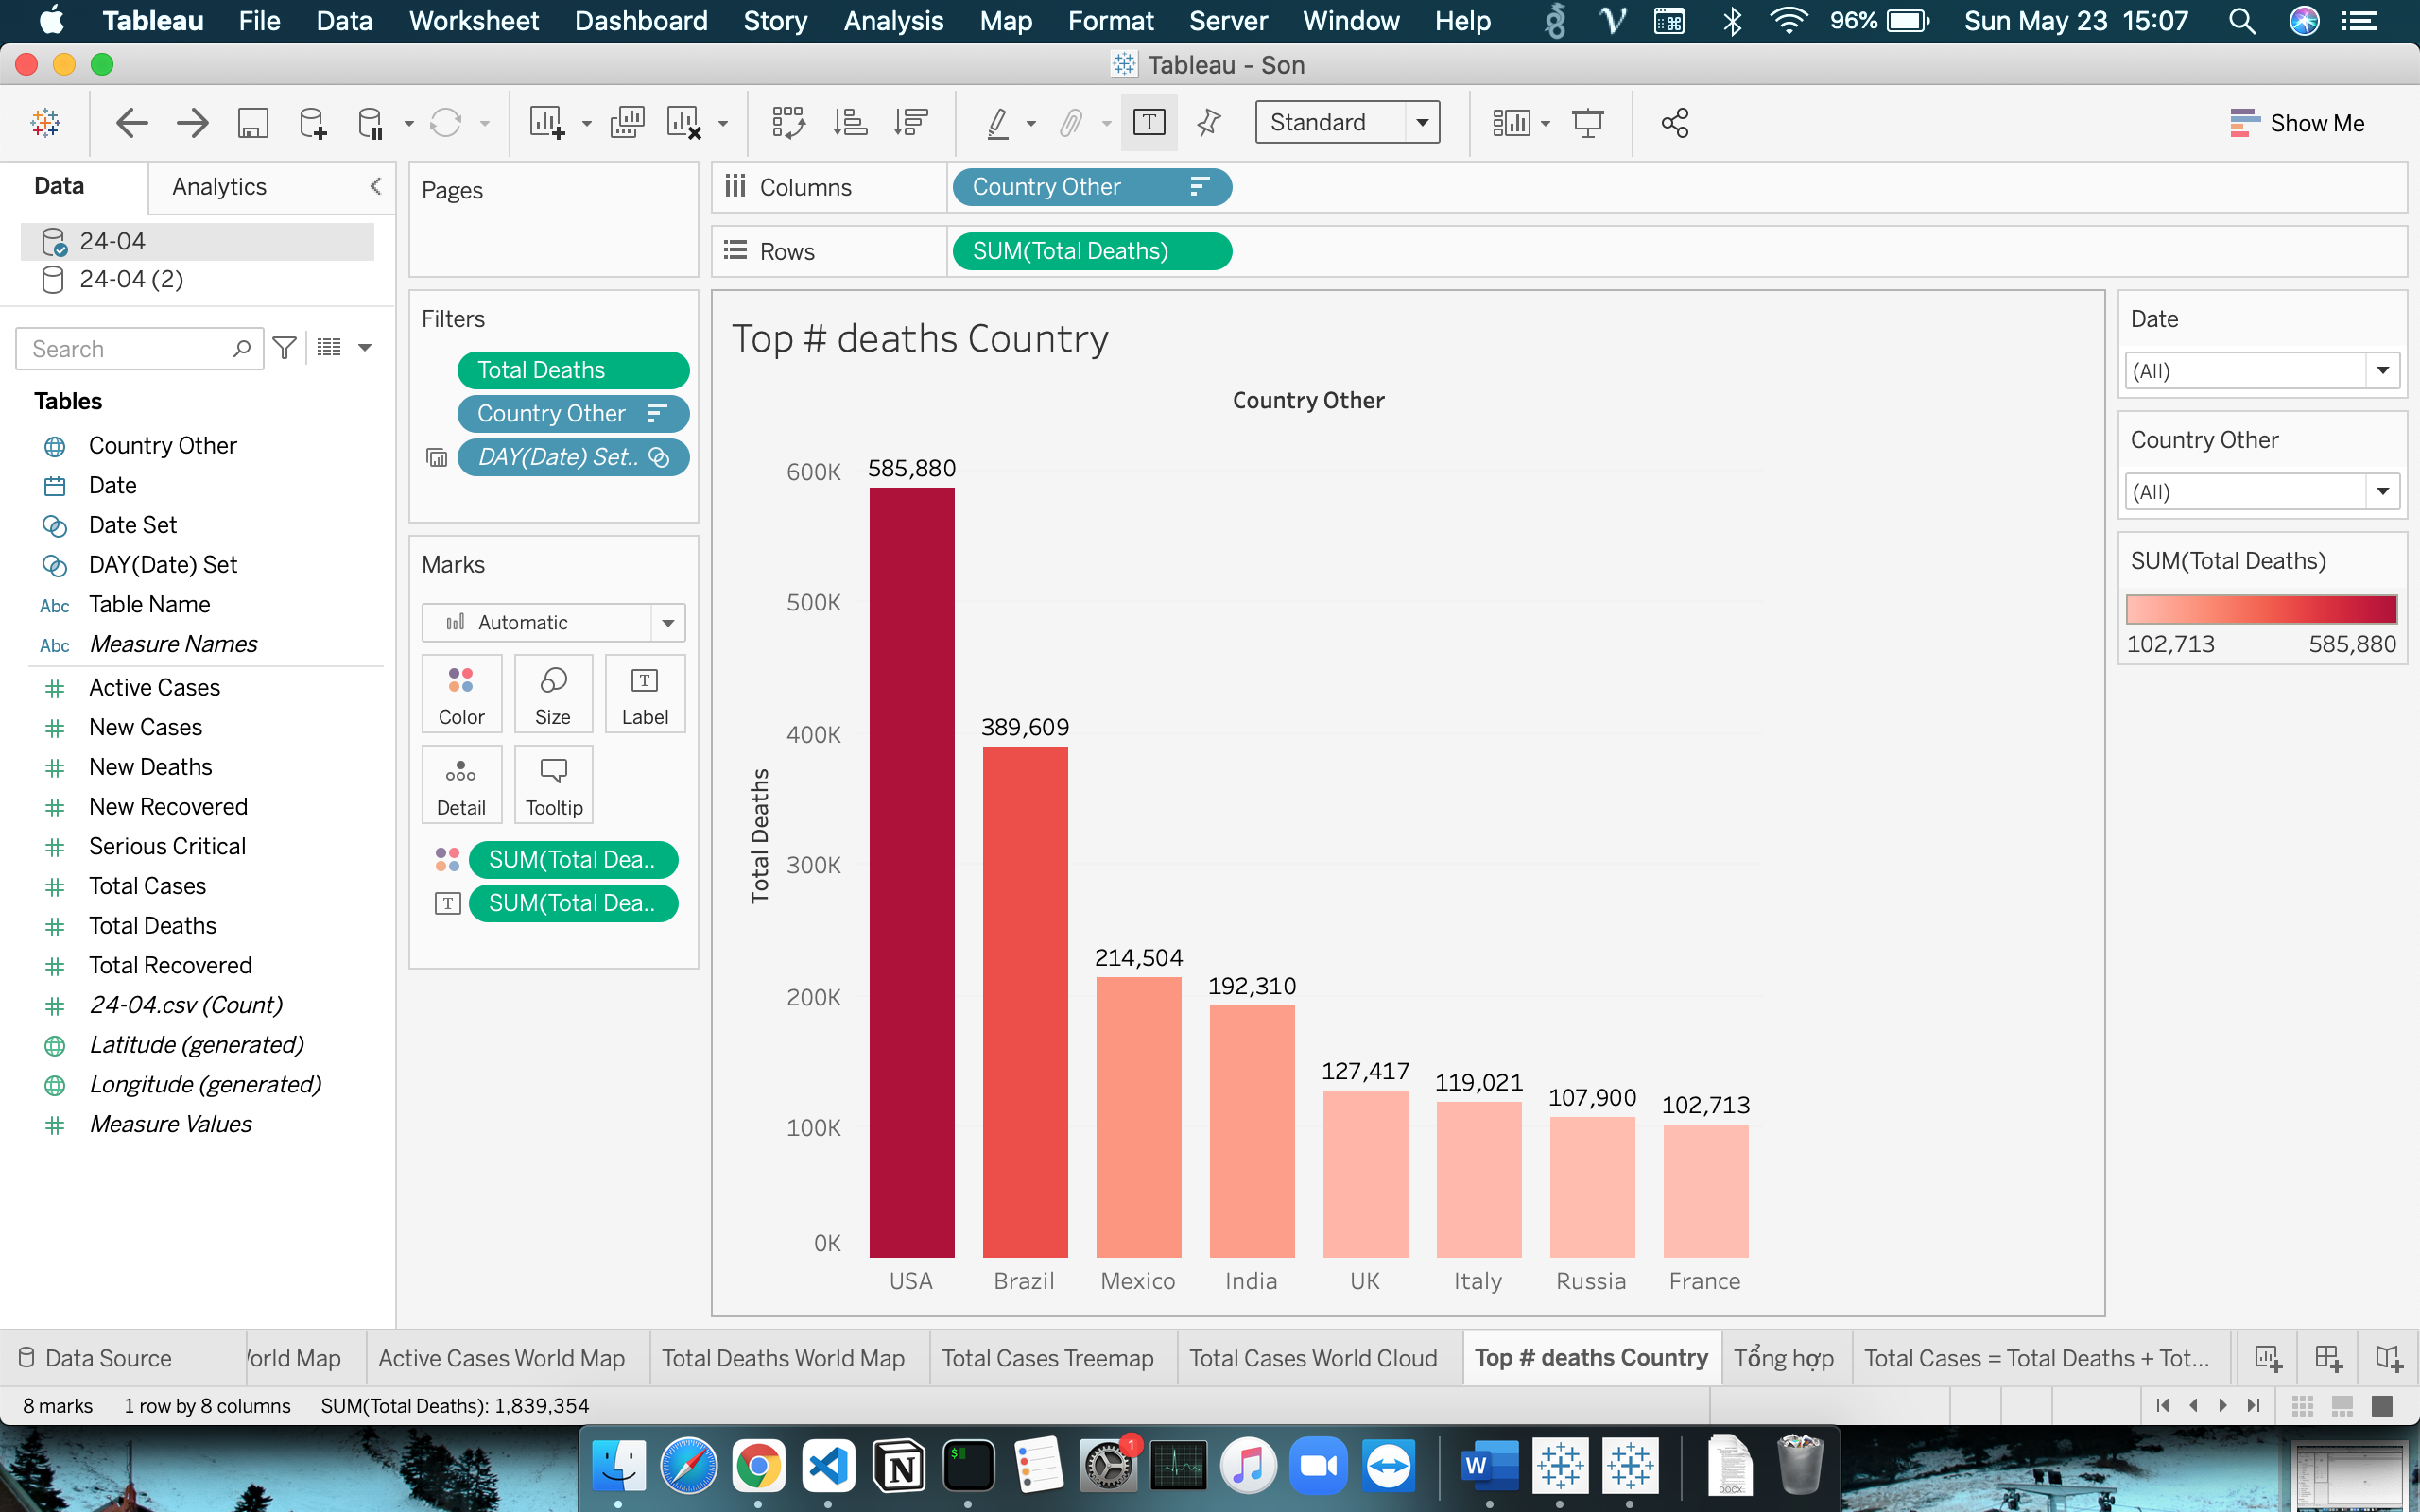
\includegraphics[scale=0.4]{img/barChartTotalDeaths.png}
                \caption{Biểu đồ biểu diễn top 8 các quốc gia có số lượng ca tử vong cao nhất}
            \end{center}
        \end{figure}
    \end{itemize}

    \item Biểu đồ cột chồng
    \begin{itemize}
        \item Lợi ích: Stacked Bar Chart thể hiện trực quan chỉ số của biến. Do đó có thể dễ dàng so sánh các nhóm dữ liệu trong cột và các cột trong biểu đồ, từ đó dễ dang đưa ra những nhận định đa chiều
        \item Nhận xét: Biểu đồ thể hiện tự tương quan giữa số lượng ca nhiễm của từng nước với nhau, ta có thể thấy rõ số lượng ca bệnh ở Mỹ nhiều gấp 3-4 lần Brazil và gấp nhiều lần so với các nước châu Âu khác. Ngoài ra, ta có thể thấy tỉ lệ số lượng ca hiện có và các ca đã bình phục, từ đó có thể suy ra được tình hình dịch của những nước đó. Ví dụ: Ấn Độ và Mỹ đang trong giai đoạn phục hồi, Pháp có thể vừa mới bùng dịch,...
        \begin{figure}[H]
            \begin{center}
                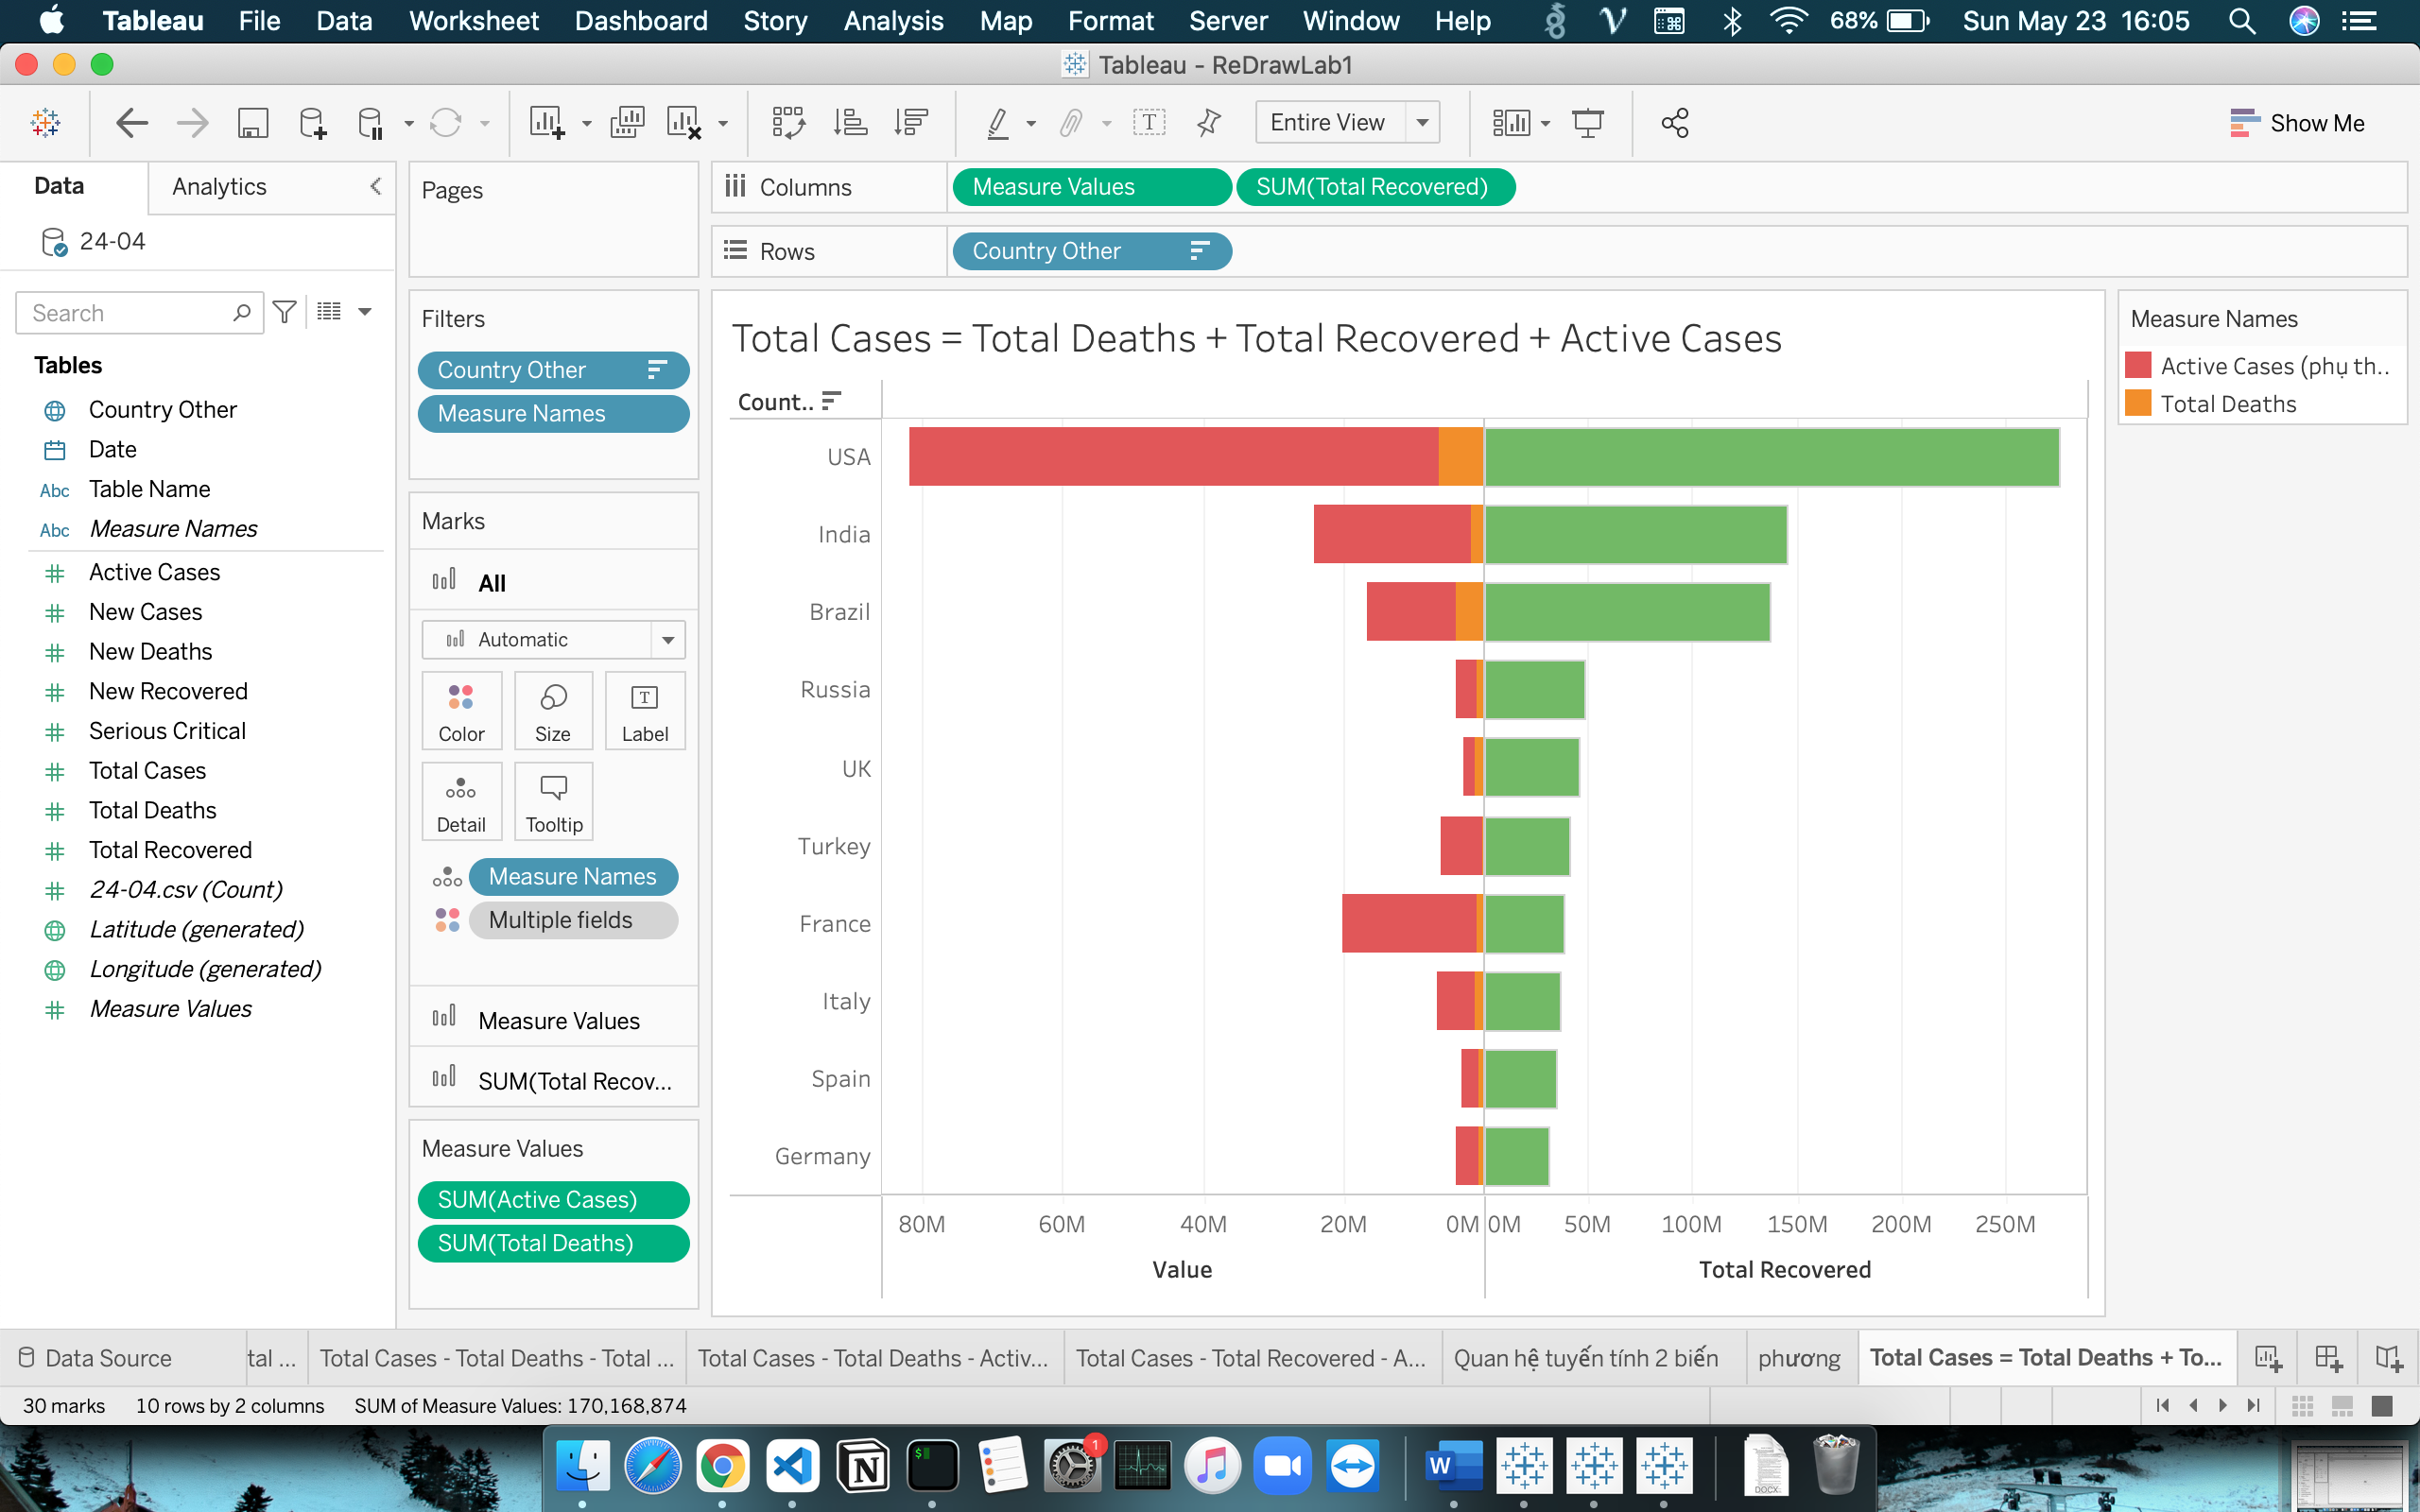
\includegraphics[scale=0.4]{img/stackedBar.png}
                \caption{Biểu đồ biểu diễn quan hệ TotalCases = TotalDeaths + TotalRecovered + ActiveCases}
            \end{center}
        \end{figure}
    \end{itemize}
\end{itemize}

\subsection{Biểu diễn Scatter Plot}

\subsubsection{Corelation matrix}

\begin{itemize}
    \item Lợi ích: Dễ dàng thấy được tương quan giữa các cặp biến với nhau
    %scatter plot giữa 2 biến trong các biến: Total Cases, Total Deaths, Total Recovered, Active Cases, Serious Cases.
    \item Các biến Total Cases, Total Deaths, Total Recovered và Active Cases có các mối tương quan với nhau khá cao ($R^2$ trên 75\%), độ tin cậy cao ($P-value$ nhỏ hơn 0.0001). Trong đó quan hệ giữa tổng số ca mắc và tổng số ca đã phục hồi cho ta thấy rằng những người nhiễm bệnh vẫn còn khả năng để chữa khỏi. Mặt khác thì số ca chết cũng cho thấy sự tương quan cao với số ca mắc: Với mỗi ca mắc mới thì sẽ tương đương với khoảng 48 ca chết mới - một con số khá đáng sợ và cần phải cảnh giác, nâng cao ý thức chống dịch trong cộng đồng.
    \begin{figure}[H]
        \begin{center}
            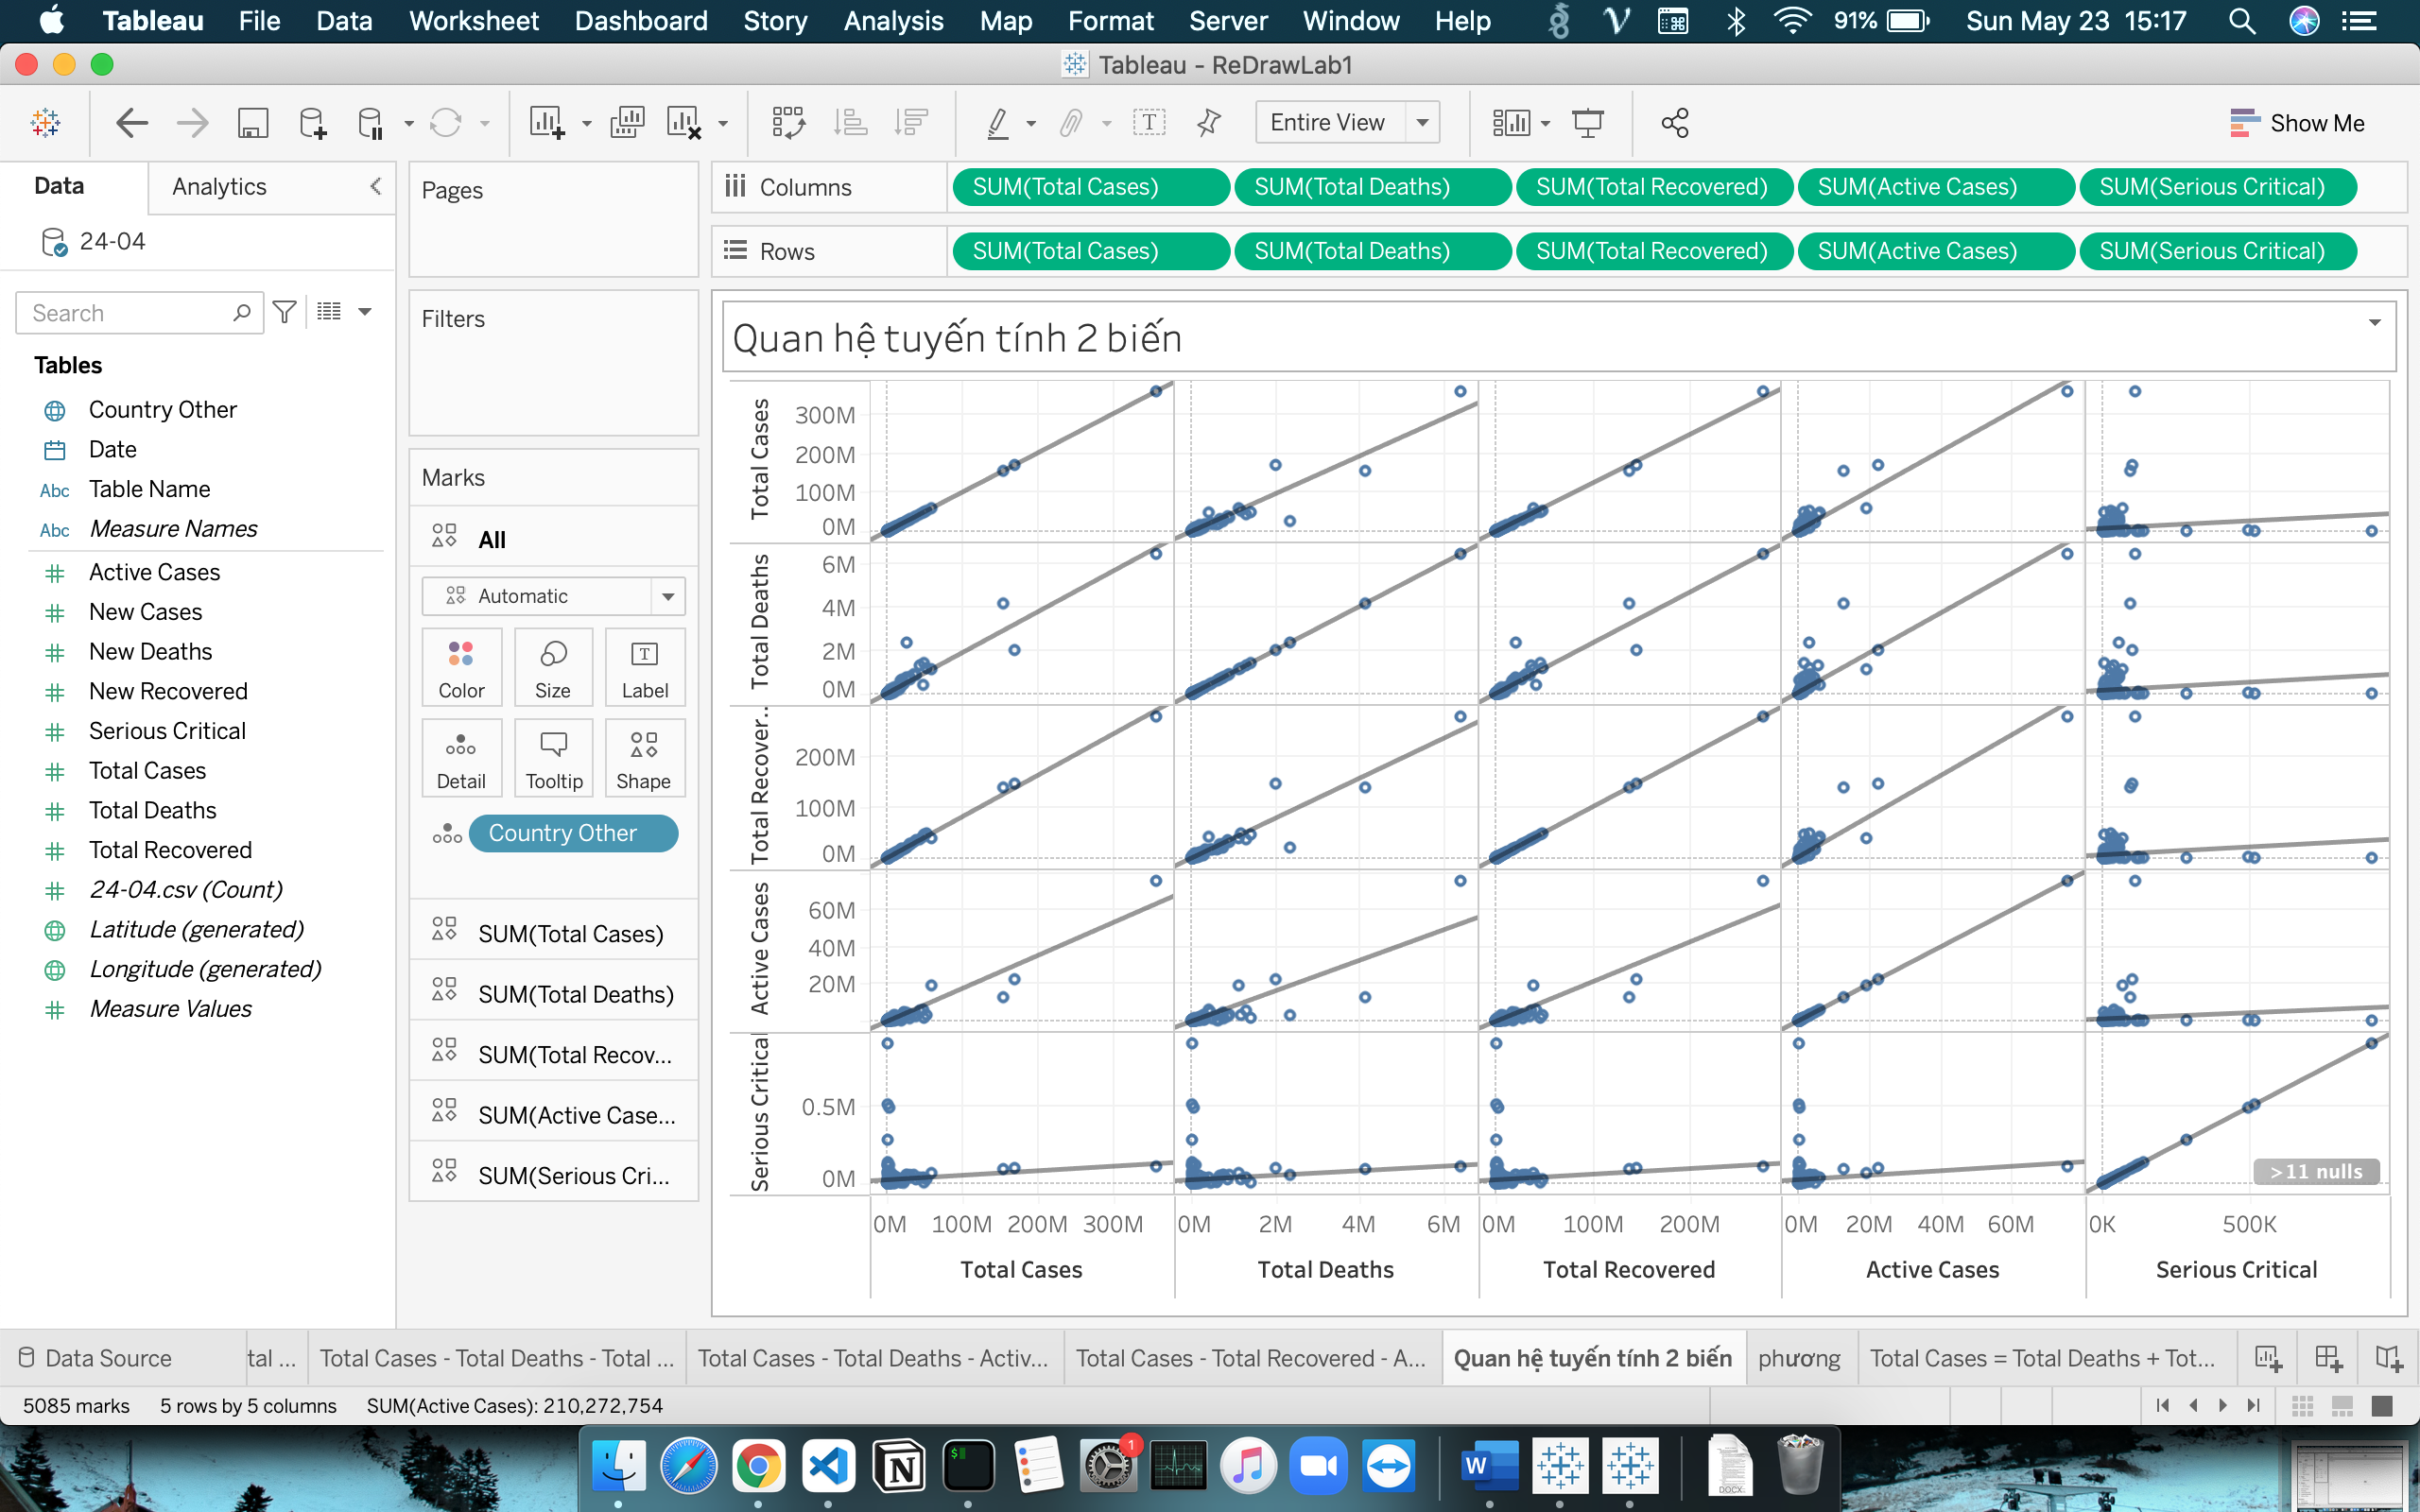
\includegraphics[scale=0.4]{img/corelation.png}
            \caption{Biểu đồ biểu diễn scatter plot giữa các cặp biến trong các biến: Total Cases, Total Deaths, Total Recovered, Active Cases, Serious Cases}
        \end{center}
    \end{figure}
\end{itemize}

\subsubsection{Biểu diễn Scatter Plot các bộ 3 và 4 biến}

\begin{itemize}
    \item Lợi ích: Scatter Plot cho phép biểu diễn tập dữ liệu theo từng điểm trên không gian hai chiều để thể hiện sự tương quan giữa ít nhất hai biến được thể hiện trên trục tung và trục hoành trong biểu đồ (như biểu diễn về Corelation ở trên). Từ đó rút ra được quan hệ giữa data là như thế nào (nagative - positive, strong - weak, linear - nonlinear, clusters, gap in values, outliers)
    \item Nhóm đã tiến hành trực quan bằng biểu đồ scatter với các bộ 3 biến và 4 biến. Chi tiết có thể xem tại các file Tableau do nhóm cung cấp
    \item Tại mục này, nhóm đề cập 1 biểu đồ về quan hệ giữa 4 biến: Total Cases - Total Deaths - Total Recovered - Active Cases
    \begin{figure}[H]
        \begin{center}
            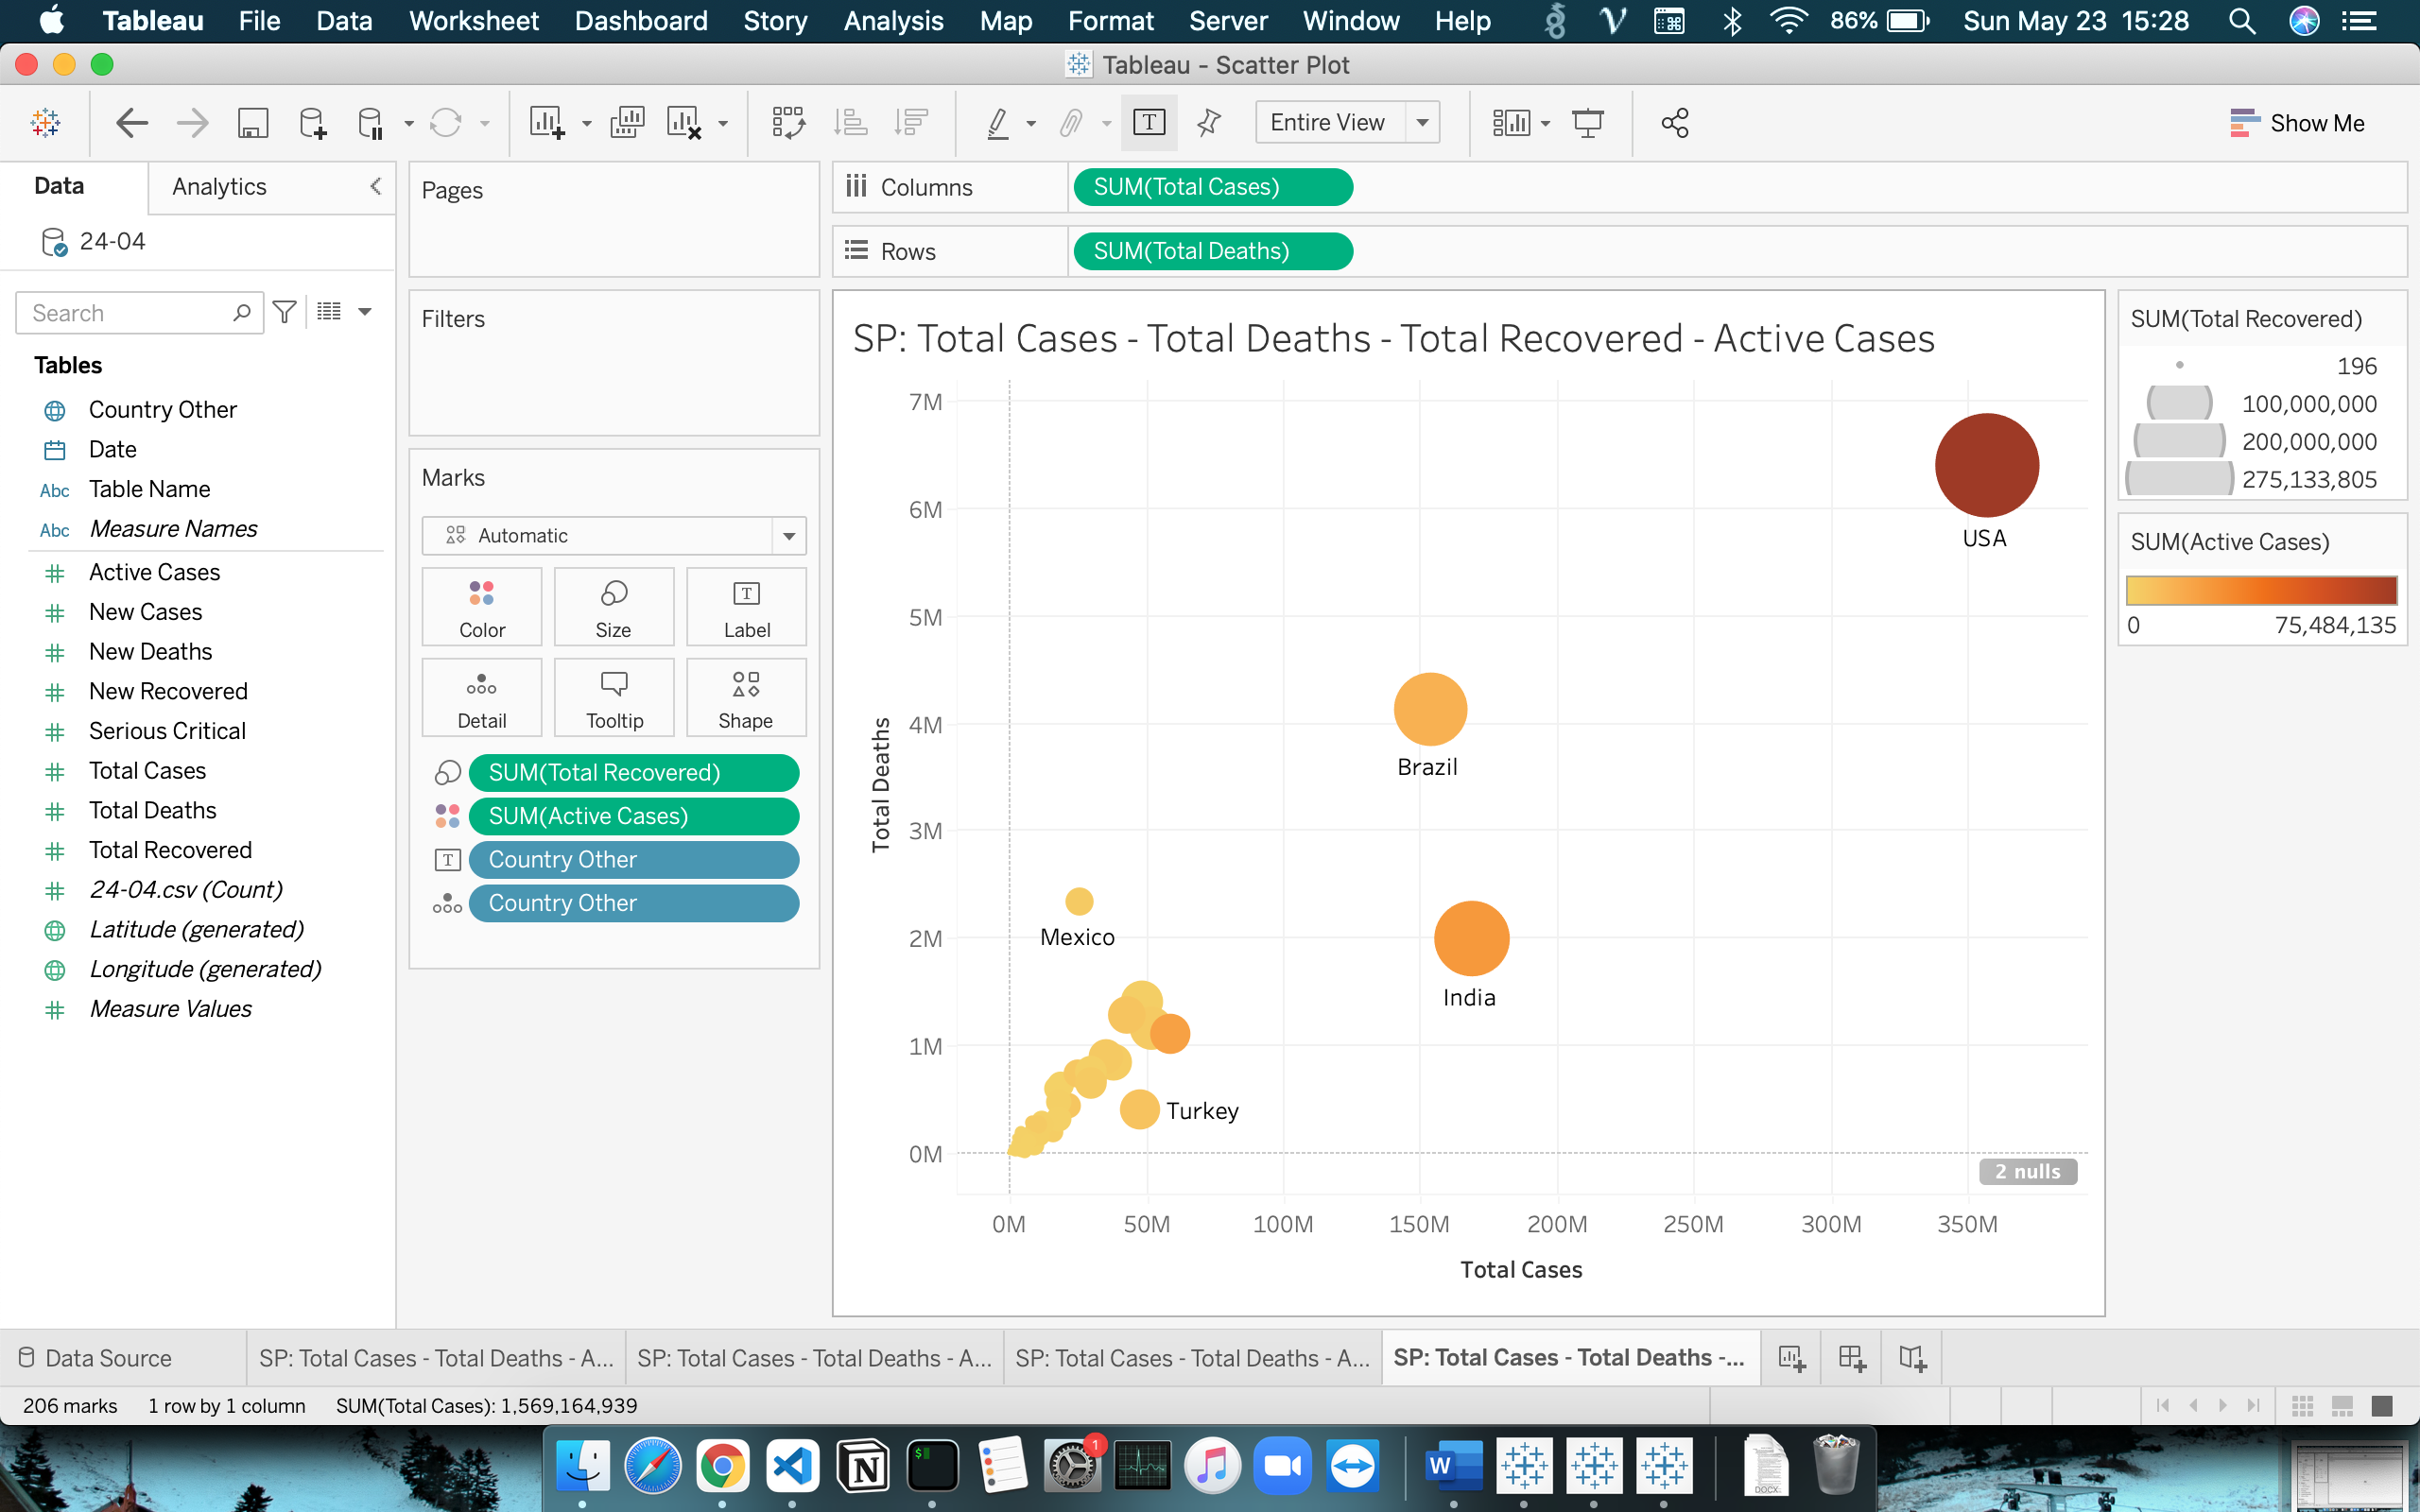
\includegraphics[scale=0.4]{img/scatter4Vars.png}
            \caption{Biểu đồ biểu diễn scatter plot giữa Total Cases - Total Deaths - Total Recovered - Active Cases}
        \end{center}
    \end{figure}

    \item Quan sát biểu đồ trên, ta rút ra một vài nhận xét sau
    \begin{itemize}
        \item Tồn tại mối quan hệ đồng biến giữa các cặp biến trong [Total Cases - Total Deaths - Total Recovered - Active Cases]
        \item Đa phần các quốc gia đều có tổng số ca nhiễm nhỏ hơn 100 triệu (quan sát trục hoành của biểu đồ) và số ca tử vong nhỏ hơn 3 triệu (quan sát trục tung của biểu đồ). Các nước này tạo thành một cụm riêng. Phần còn lại là 3 nước Mỹ, Ấn Độ, Brazil
        \item Sự chênh lệch rất lớn của các biến giữa các nước Mỹ, Ấn Độ, Brazil và các nước khác trong biểu đồ. Nhìn nhận một cách tích cực, 3 quốc gia này đang dần hồi phục sau đại dịch khi có số ca hồi phục cao nhất trên thế giới. Tuy nhiên, nếu nhìn theo chiều hướng tiêu cực, đây cũng là 3 quốc gia có số người chết và số người đang nằm điều trị lớn nhất thế giới. Trong đó, số ca nằm điều trị đang tăng theo chiều hướng khó kiểm soát. Có thể dự đoán thêm rằng, các dịch vụ y tế của 3 nước này sẽ chịu áp lực rất lớn, thậm chí quá tải và dừng hoạt động nếu chiều hướng cứ tiếp tục tăng tuyến tính như trên biểu đồ
    \end{itemize}
\end{itemize}

\subsubsection{Biểu diễn Line Chart}

\begin{itemize}
    \item Lợi ích: Line Chart biểu diễn tốt các dữ liệu có tính liên tục, minh họa rõ nét xu hướng thay đổi của các chỉ số theo thời gian, giúp dễ dàng quan sát sự dao động của biến. Từ đó đưa ra dự đoán về dữ liệu trong tương lai. Ngoài ra, khi so sánh các tập dữ liệu, Line Chart thể hiện rõ sự chênh lệch và các mốc giao nhau giữa mỗi đường
    \begin{figure}[H]
        \begin{center}
            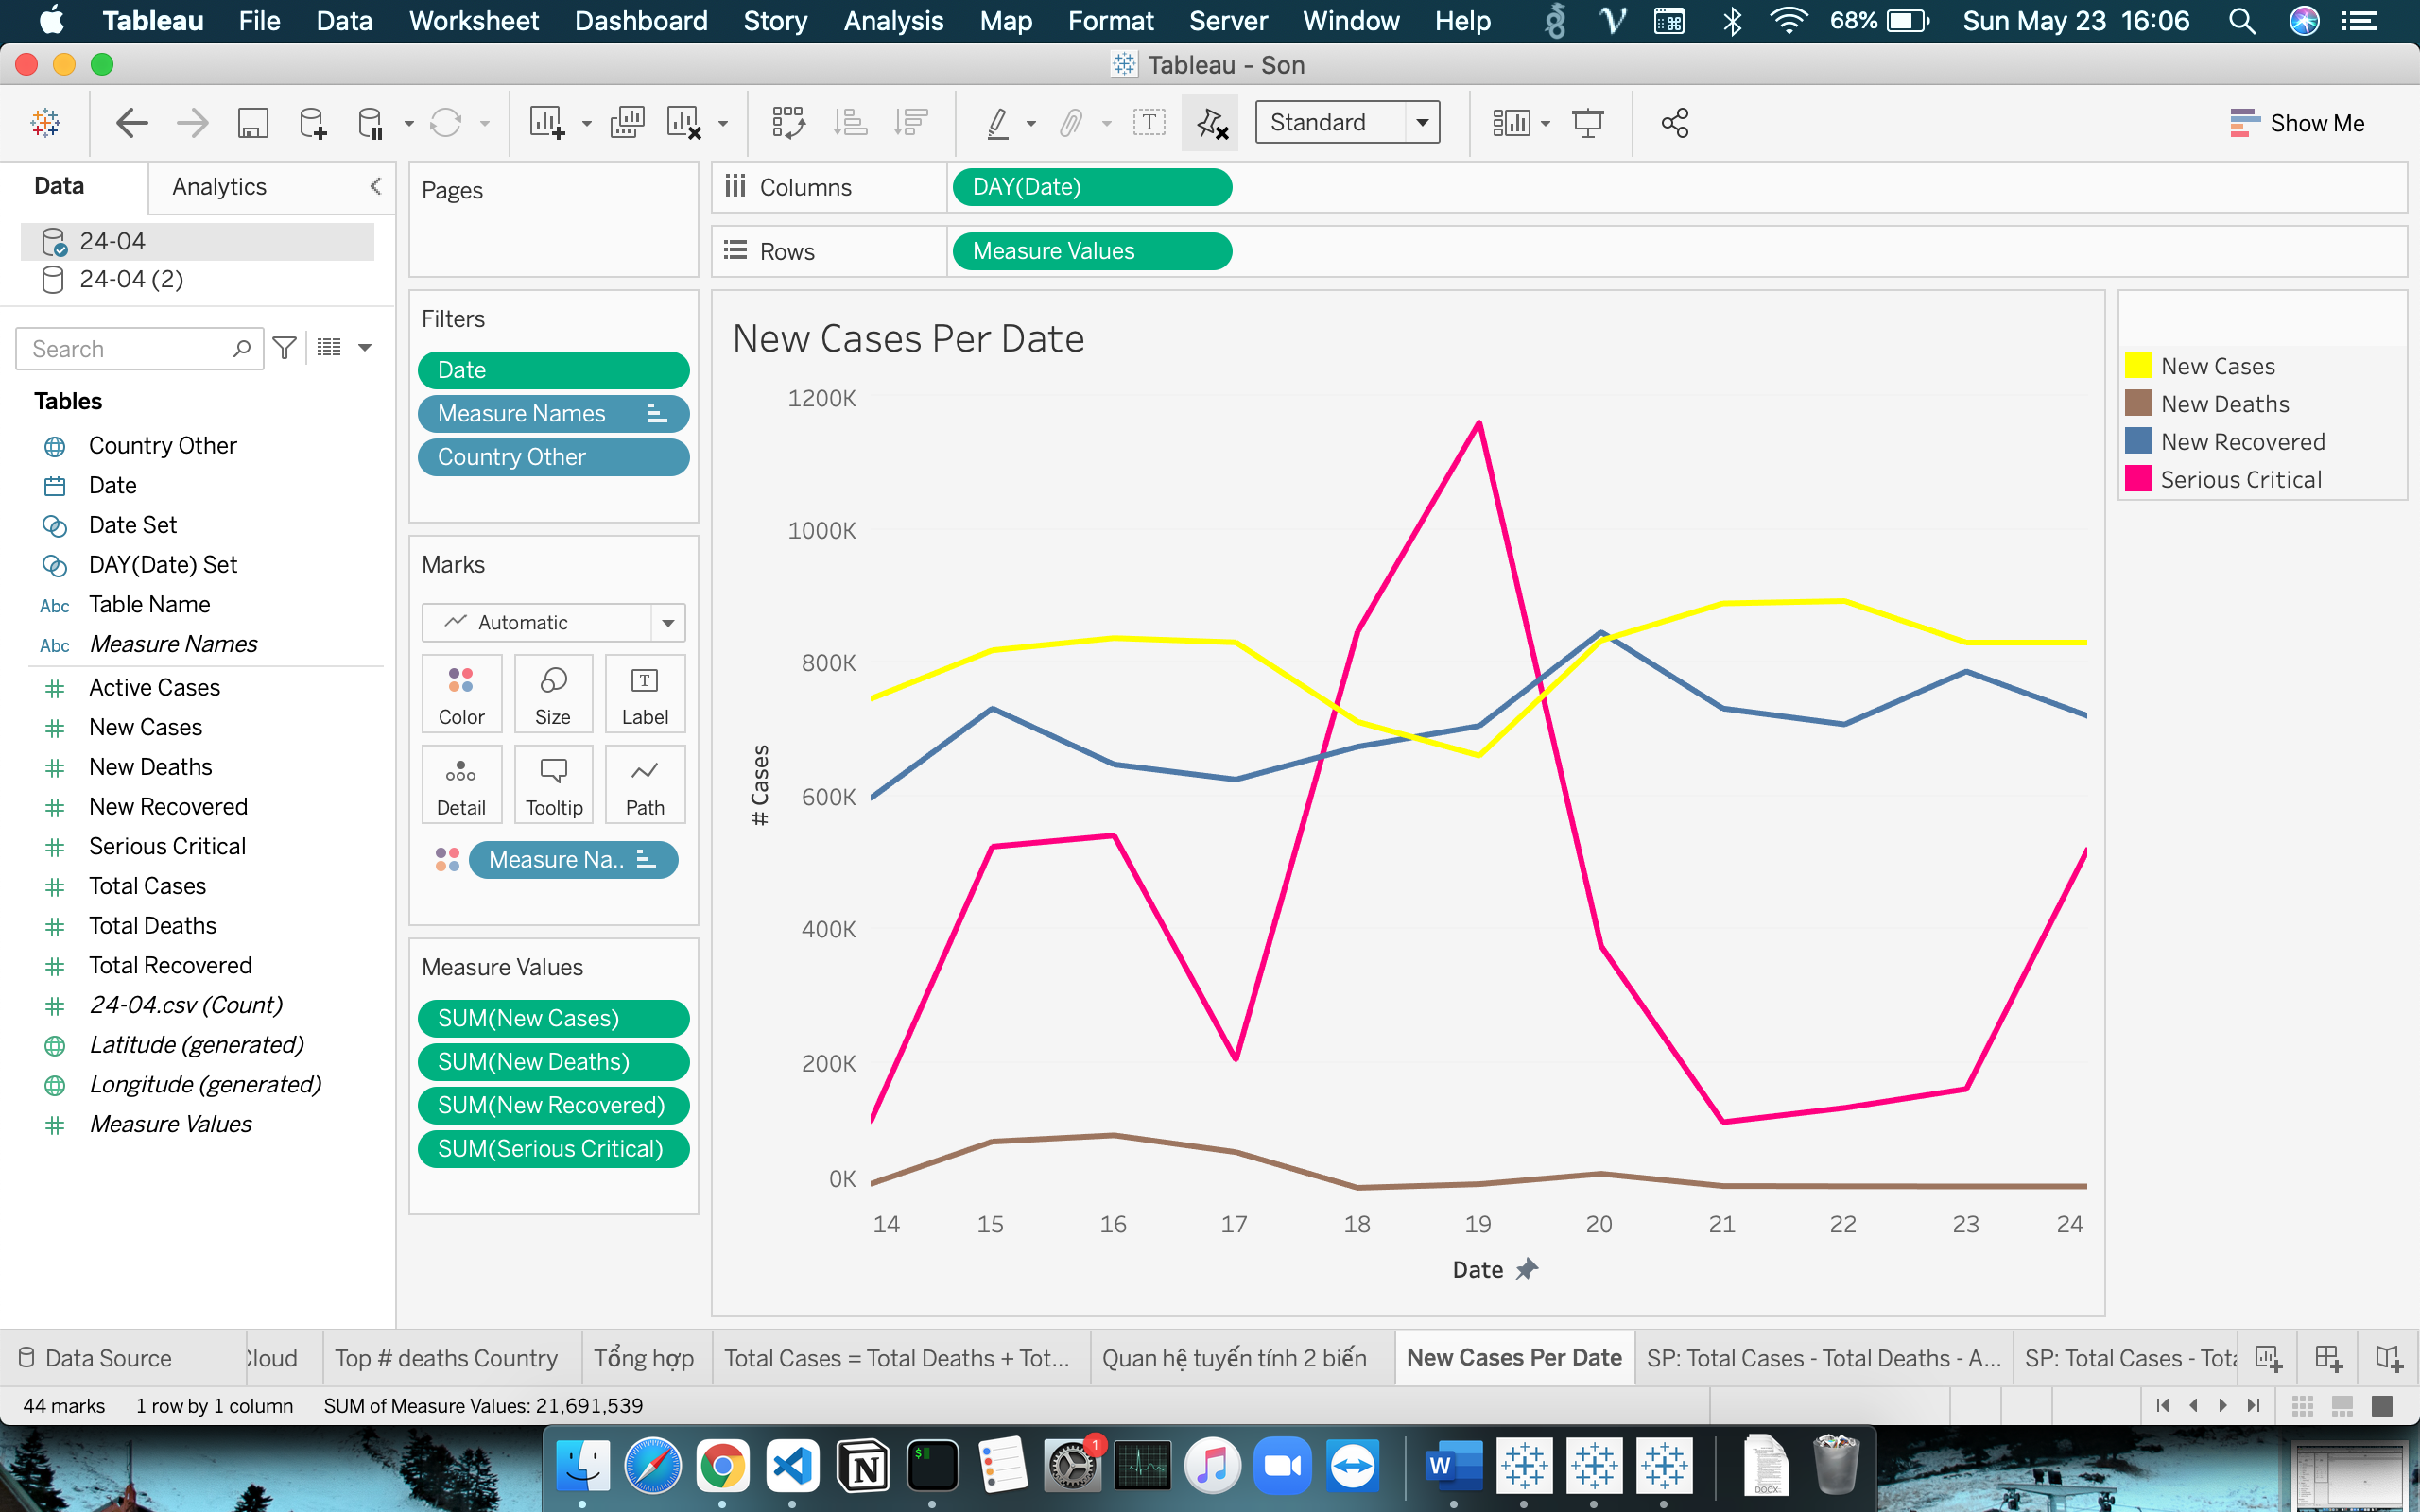
\includegraphics[scale=0.4]{img/lineChart1.png}
            \caption{Biểu đồ biểu diễn biến động theo ngày của các thuộc tính New Cases, New Deaths, New Recovered và Serious Critical}
        \end{center}
    \end{figure}

    \item Nhận xét: Biểu đồ cho ta thấy được trong 10 ngày từ 14-24/02:
    \begin{itemize}
        \item Số lượng ca bệnh mới, ca hồi phục dao động liên tục nhưng không có xu hướng tăng hay giảm
        \item Các ca nguy hiểm dao động mạnh và có dấu hiệu tăng trong vài ngày tiếp theo
        \item Số lượng ca tử xong có xu hướng giảm nhẹ
        \item Về tương quan giữa số lượng ca bệnh, số lượng ca hồi phục mỗi ngày xấp xỉ ca mắc mới, tỉ lệ ca tử vong thấp
    \end{itemize}
\end{itemize}

\subsubsection{Biểu diễn World Map}

\begin{itemize}
    \item Lợi ích
    \begin{itemize}
        \item Giúp người xem dễ dàng thấy được phân bố của dịch bệnh ở các quốc gia trên thế giới
        \item Từ đó dễ dàng nhận biết được các "ổ dịch" trên thế giới
        \item Khả năng so sánh nhanh số ca mắc ở các khu vực
    \end{itemize}

    \begin{figure}[H]
        \begin{center}
            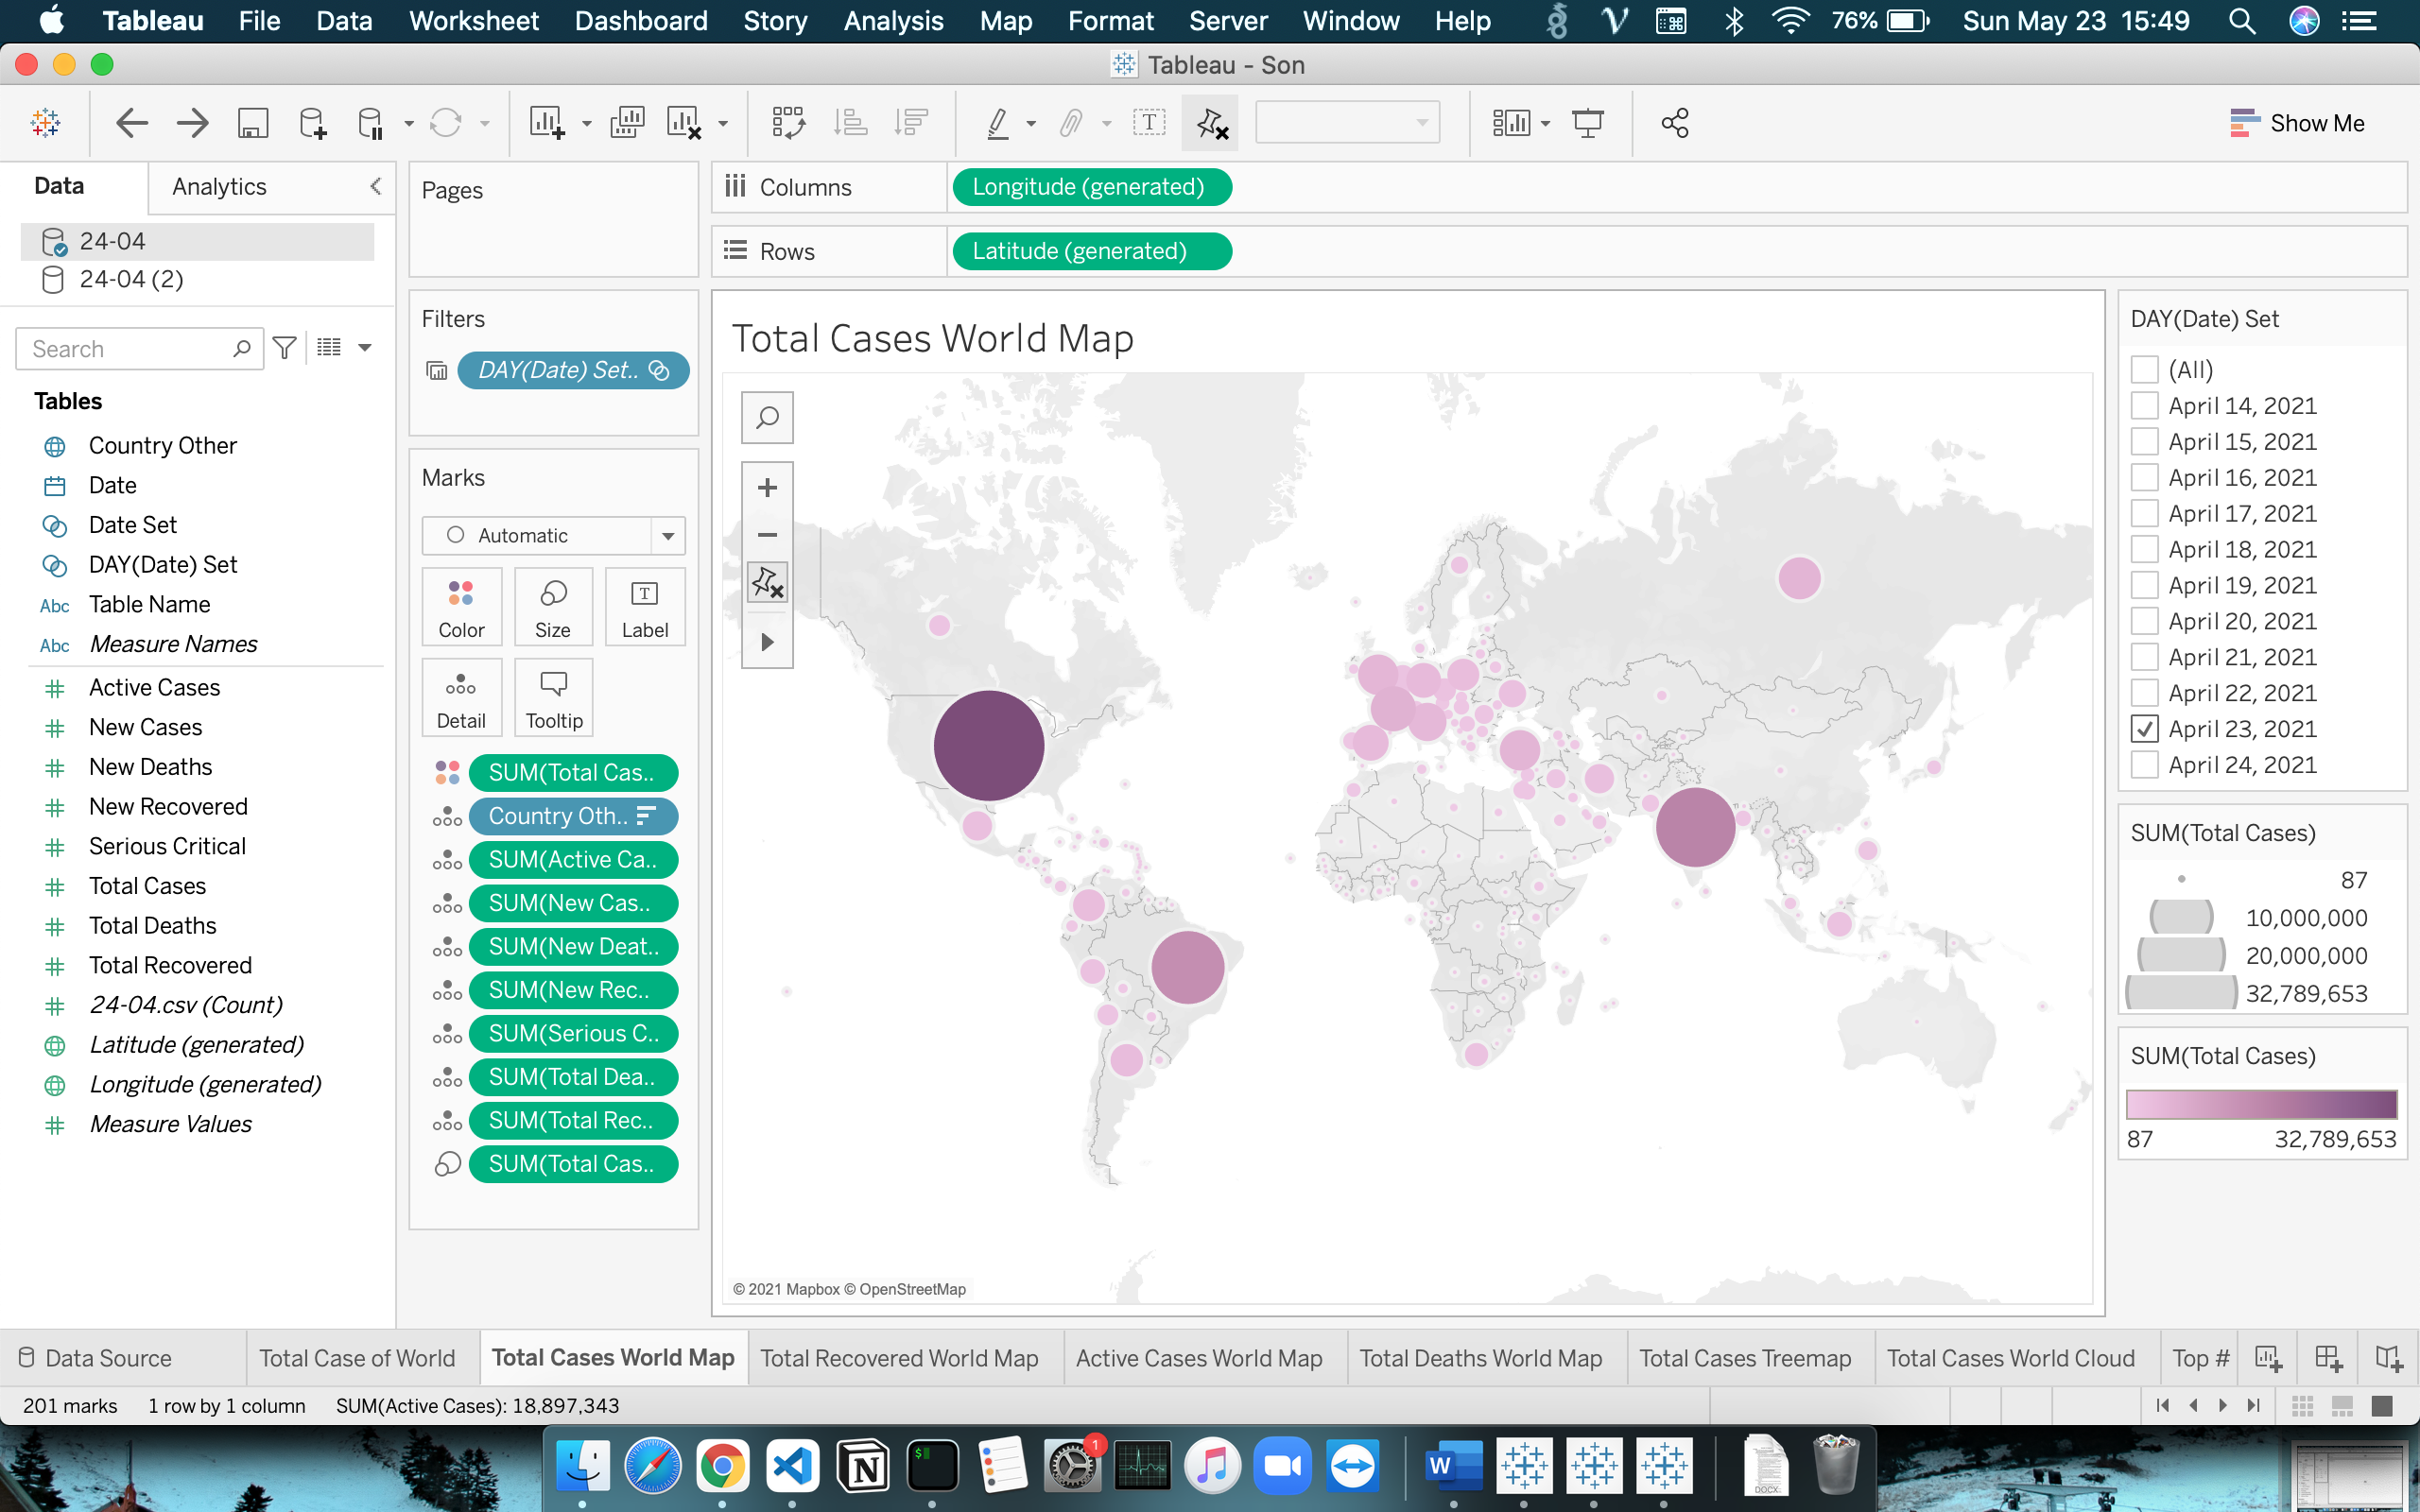
\includegraphics[scale=0.4]{img/worldMap.png}
            \caption{Biểu đồ biểu diễn phân bố dịch theo tổng số ca mắc trên toàn thế giới}
        \end{center}
    \end{figure}

    \item Nhận xét:
    \begin{itemize}
        \item Có thể thấy các ổ dịch lớn trên thế giới tập trung ở Bắc Mĩ, Nam Mỹ, Tây Âu và Nam Á
        \item Các nước dẫn đầu là Mỹ, Ấn Độ, Brazil
        \item Ổ dịch ở châu Âu có ca mắc của từng nước tuy là ít nhưng lại tập trung nhiều nước. Lý giải cho việc này là sự thiếu ý thức trong việc đeo khẩu trang và tụ tập nơi đông người
        \item Ấn Độ có số ca mắc tăng chóng mặt từ những tháng đầu năm đến nay do việc tổ chức các lễ hội đông người cùng sự tụ tập ăn bằng tay khiến dịch bệnh lây lan không kiểm soát
        \item Mỹ "vượt mặt" mọi quốc gia về tất cả các chỉ số bệnh dịch. Đây vừa là kết quả của một nền y tế chất lượng cao (số ca hồi phục lớn nhất thế giới) vừa là hậu quả của việc điều hành nhà nước (người lãnh đạo cũ của đất nước kêu gọi mọi người không đeo khẩu trang và đã từng bị nhiễn covid)
    \end{itemize}

    \item Ngoài biểu đồ thể hiện tổng số ca mắc trên thế giới, vẫn còn các biểu diễn khác của world map. Người đọc có thể xem chi tiết trong file Tableau do nhóm cung cấp
\end{itemize}

\subsubsection{Dashboard}

\begin{itemize}
    \item Từ các biểu đồ trên, ta có thể thống kê thành một dashboard như sau
    \begin{figure}[H]
        \begin{center}
            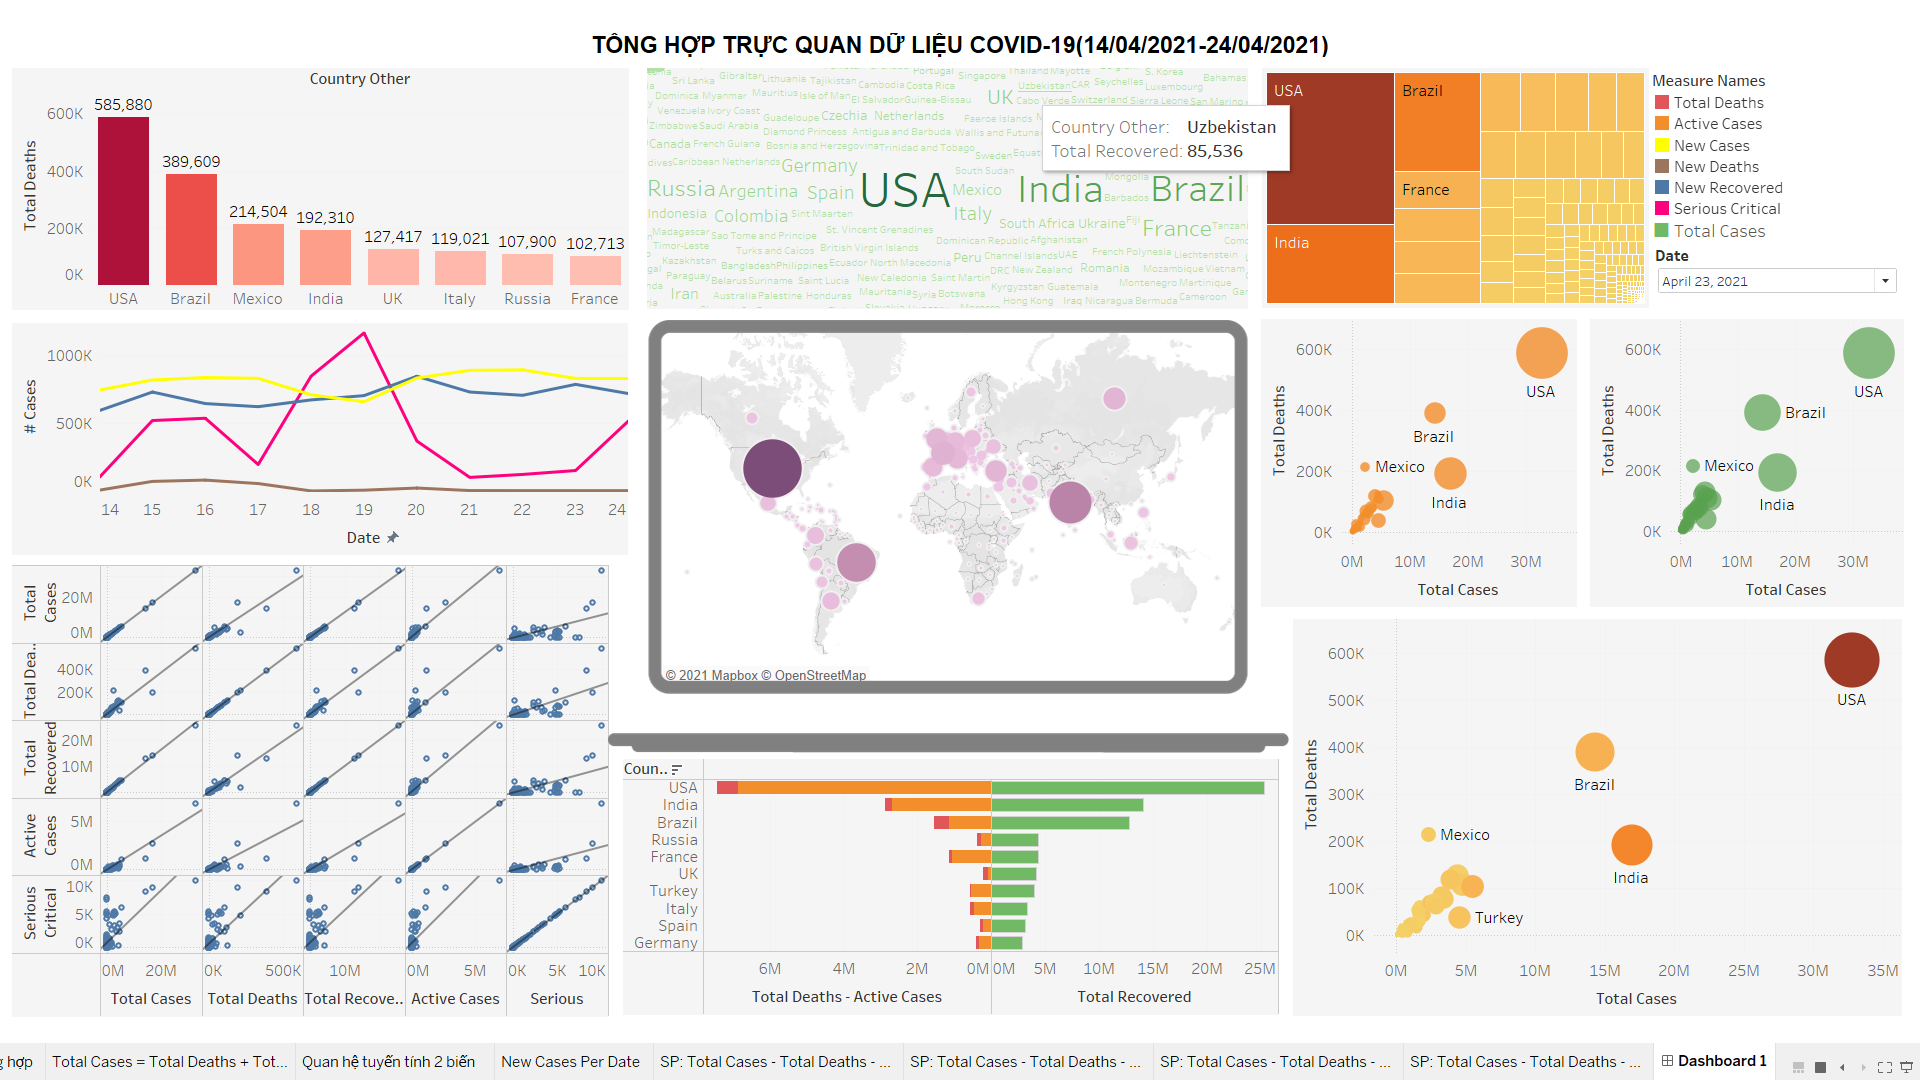
\includegraphics[scale=0.25]{img/dashboard1.png}
            \caption{Dashboard tổng hợp biểu trực quan dữ liệu Covid19 (14/04/2021 - 24/04/2021)}
        \end{center}
    \end{figure}
\end{itemize}

\clearpage

\section{Tham khảo}

\begin{itemize}
    \item \url{https://tableau.bsdinsight.com/}
    \item \url{https://www.bacs.vn/vi/blog/cong-cu-ho-tro/tableau-la-gi-nhung-dieu-can-biet-ve-tableau-data-visualization-6145.html}
    \item \url{https://www.youtube.com/channel/UCMUbHNZctxb65xlTZbu1laQ/featured}
\end{itemize}

\end{document}